\documentclass[12pt,twoside,a4paper]{book}

% ---------------------------------------------------------------------------- %
% Pacotes 
\usepackage[T1]{fontenc}
\usepackage[portuguese]{babel}
\usepackage{floatrow}
\newfloatcommand{capbtabbox}{table}[][\FBwidth]
\usepackage{blindtext}
\setcounter{tocdepth}{3}
\setcounter{secnumdepth}{3}
% \usepackage[latin1]{inputenc}
\usepackage[utf8x]{inputenc}
\usepackage[pdftex]{graphicx}           % usamos arquivos pdf/png como figuras
\usepackage[toc,page]{appendix}
\usepackage{setspace}                   % espaçamento flexível
\usepackage{float}
\usepackage{indentfirst}                % indentação do primeiro parágrafo
\usepackage{makeidx}                    % índice remissivo
\usepackage[nottoc,notlot,notlof]{tocbibind}         % acrescentamos a bibliografia/indice/conteudo no Table of Contents
\usepackage{courier}  % usa o Adobe Courier no lugar de Computer Modern Typewriter
\usepackage{vowel}
\usepackage{type1cm}                    % fontes realmente escaláveis
\usepackage{pdfpages}
\usepackage{tipa}                       % para utilizar simbolos foneticos
\usepackage{listings}                   % para formatar código-fonte (ex. em Java)
\usepackage{titletoc}
%\usepackage[landscape,dvips]{geometry}
\usepackage{tabularx} 
\addto\captionsportuguese{% Replace "english" with the language you use
  \renewcommand{\contentsname}%
    {Sumário}%
}
\newcommand{\aup}{\textsuperscript}
\interfootnotelinepenalty=10000
\usepackage{lastpage}
\usepackage{tipa}
\let\ipa\textipa
\usepackage[utf8]{inputenc}
\newcommand{\BlankCell}{}
\usepackage{lmodern}
\usepackage{amsmath}
\usepackage{amsfonts}
\usepackage{booktabs}
\usepackage{bm}
\usepackage{epigraph}
\setlength\epigraphwidth{.6\textwidth}
\setlength\epigraphrule{0pt}

%\usepackage[bf,small,compact]{titlesec} % cabeçalhos dos títulos: menores e compactos
\usepackage[fixlanguage]{babelbib}
\usepackage[font=normalsize,format=plain,labelfont=bf,up,textfont=it,up,skip=0pt]{caption}
\usepackage[usenames,svgnames,dvipsnames]{xcolor}
\usepackage[a4paper,top=2.54cm,bottom=2.0cm,left=2.0cm,right=2.54cm]{geometry} % margens
%\usepackage[pdftex,plainpages=false,pdfpagelabels,pagebackref,colorlinks=true,citecolor=black,linkcolor=black,urlcolor=black,filecolor=black,bookmarksopen=true]{hyperref} % links em preto
\usepackage[pdftex,plainpages=false,pdfpagelabels,pagebackref,colorlinks=true,citecolor=black,linkcolor=black,urlcolor=black,filecolor=black,bookmarksopen=true]{hyperref} % links coloridos
\usepackage[all]{hypcap}                    % soluciona o problema com o hyperref e capitulos
\usepackage[round,sort,nonamebreak]{natbib} % citação bibliográfica textual(plainnat-ime.bst)
%\setcitestyle{numbers}
\usepackage{pgfplots}
\usepackage{hyperref}
\fontsize{70}{72}\usefont{OT1}{cmr}{m}{n}
{\selectfont}
\nocite{*}

% ---------------------------------------------------------------------------- %
% Cabeçalhos similares ao TAOCP de Donald E. Knuth
\usepackage{fancyhdr}
\pagestyle{fancy}
\fancyhf{}

% new commands------------------------
\usepackage{subcaption}
\newcommand{\vect}[1]{\bm{#1}}
\newcommand{\myprime}[1]{{#1}^{\prime}}
\newcommand{\grad}[2]{\nabla_{#1} {#2}}
\newcommand{\dotp}[2]{{#1}^{\top}{#2}}
\newcommand{\dotpPright}[2]{{#1}^{\top}\left({#2}\right)}
\newcommand{\outerp}[2]{\left({#1}\right){#2}^{\top}}
\newcommand{\Jacobian}[2]{\frac{\partial #1}{\partial #2}}
\newcommand{\Vocab}{\mathbb{V}}
\newcommand{\corpus}{\mathbb{C}}
\newcommand{\A}{\mathcal{A}}
\DeclareMathOperator*{\argmin}{arg\,min}
 \DeclareMathOperator*{\argmax}{arg\,max}
\DeclareMathOperator{\E}{\mathbb{E}}

% new commands------------------------

\renewcommand{\chaptermark}[1]{\markboth{\MakeUppercase{#1}}{}}
\renewcommand{\sectionmark}[1]{\markright{\MakeUppercase{#1}}{}}
\renewcommand{\headrulewidth}{0pt}

% ---------------------------------------------------------------------------- %
\graphicspath{{./figuras/}}             % caminho das figuras (recomendável)
\frenchspacing                          % arruma o espaço: id est (i.e.) e exempli gratia (e.g.) 
\urlstyle{same}                         % URL com o mesmo estilo do texto e não mono-spaced
\makeindex                              % para o índice remissivo
\raggedbottom                           % para não permitir espaços extra no texto
\fontsize{70}{72}\usefont{OT1}{cmr}{m}{n}{\selectfont}
\cleardoublepage
\large

% ---------------------------------------------------------------------------- %
% Opções de listing usados para o código fonte
% Ref: http://en.wikibooks.org/wiki/LaTeX/Packages/Listings
\lstset{ %
language=Python,                  % choose the language of the code
basicstyle=\footnotesize,       % the size of the fonts that are used for the code
numbers=left,                   % where to put the line-numbers
numberstyle=\footnotesize,      % the size of the fonts that are used for the line-numbers
stepnumber=1,                   % the step between two line-numbers. If it's 1 each line will be numbered
numbersep=5pt,                  % how far the line-numbers are from the code
showspaces=false,               % show spaces adding particular underscores
showstringspaces=false,         % underline spaces within strings
showtabs=false,                 % show tabs within strings adding particular underscores
frame=single,	                % adds a frame around the code
framerule=0.6pt,
tabsize=2,	                    % sets default tabsize to 2 spaces
captionpos=b,                   % sets the caption-position to bottom
breaklines=true,                % sets automatic line breaking
breakatwhitespace=false,        % sets if automatic breaks should only happen at whitespace
escapeinside={\%*}{*)},         % if you want to add a comment within your code
backgroundcolor=\color[rgb]{1.0,1.0,1.0}, % choose the background color.
rulecolor=\color[rgb]{0.8,0.8,0.8},
extendedchars=true,
xleftmargin=10pt,
xrightmargin=10pt,
framexleftmargin=10pt,
framexrightmargin=10pt
}

% Additional packages
\usepackage{lscape}

\usepackage{booktabs}
\usepackage{graphicx}
% \usepackage[table,xcdraw]{xcolor}
\usepackage{colortbl}
\usepackage{algpseudocode}
\usepackage{soul}
\usetikzlibrary{matrix,chains,positioning,decorations.pathreplacing,arrows}

%circle table
\newcommand*\circled[1]{\tikz[baseline=(char.base)]{% <---- BEWARE
            \node[shape=circle,draw,inner sep=2pt] (char) {#1};}}

% Declaracoes em Português
\algrenewcommand\algorithmicend{\textbf{fim}}
\algrenewcommand\algorithmicdo{\textbf{faça}}
\algrenewcommand\algorithmicwhile{\textbf{enquanto}}
\algrenewcommand\algorithmicfor{\textbf{para}}
\algrenewcommand\algorithmicif{\textbf{se}}
\algrenewcommand\algorithmicthen{\textbf{então}}
\algrenewcommand\algorithmicelse{\textbf{senão}}
\algrenewcommand\algorithmicreturn{\textbf{devolve}}
\algrenewcommand\algorithmicfunction{\textbf{função}}

% Rearranja os finais de cada estrutura
\algrenewtext{EndWhile}{\algorithmicend\ \algorithmicwhile}
\algrenewtext{EndFor}{\algorithmicend\ \algorithmicfor}
\algrenewtext{EndIf}{\algorithmicend\ \algorithmicif}
\algrenewtext{EndFunction}{\algorithmicend\ \algorithmicfunction}
% O comando For, a seguir, retorna 'para #1 -- #2 até #3 faça'
\algnewcommand\algorithmicto{\textbf{até}}
\algrenewtext{For}[3]%
{\algorithmicfor\ #1 $\gets$ #2 \algorithmicto\ #3 \algorithmicdo}

\usepackage{adjustbox}
\usepackage{fancyvrb}
\usepackage{amsmath}
\usepackage{amsthm}
\usepackage{amssymb}
\usepackage{breakcites}

\usepackage{cases}
\newcommand\tab[1][1cm]{\hspace*{#1}}
\usepackage[ruled,vlined,linesnumbered]{algorithm2e}
\SetKwComment{Comment}{$\triangleright$\ }{}
\usepackage{tikz}
\usetikzlibrary{shapes,arrows,positioning,fit,backgrounds, arrows.meta}
\newcommand{\empt}[2]{$#1^{\langle #2 \rangle}$}
% Tikzstyles for Computation Graphs

% nodes
\tikzstyle{noop} = [circle, draw=none, fill=red, minimum size = 10pt]
\tikzstyle{op} = [circle, draw=red, line width=1.5pt, fill=red!70, text=black, text centered, font=\bf \normalsize, minimum size = 25pt]

\tikzstyle{opintense} = [circle, draw=red, line width=1.5pt, fill=red!150, text=black, text centered, font=\bf \normalsize, minimum size = 25pt]


%new style
\tikzstyle{gp} = [circle, draw=red, line width=4pt, text=black, text centered, font=\bf \normalsize, minimum size = 4.cm]

\tikzstyle{box} = [rectangle, draw=red, line width=1.5pt, fill=red!70, text=black, align=center, font=\bf \normalsize, minimum size = 45pt]

\tikzstyle{box2} = [rectangle, draw=black, line width=0.9pt, text=black, align=center, font=\bf \normalsize, minimum size = 20pt]

\tikzstyle{box3} = [rectangle, draw=black, line width=0.9pt, fill=black, text=black, align=center, font=\bf \normalsize, minimum size = 20pt]

\tikzstyle{state} = [circle, draw=blue, line width=1.5pt, fill=blue!70, text=black, text centered, font=\bf \normalsize, minimum size = 25pt]

\tikzstyle{output} = [circle, draw=purple, line width=1.5pt, fill=purple!70, text=black, text centered, font=\bf \normalsize, minimum size = 25pt]


\tikzstyle{gradient} = [circle, draw=nephritis, line width=1.5pt, fill=nephritis!60, text=black, text centered, font=\bf \normalsize, minimum size = 25pt]
\tikzstyle{textonly} = [draw=none, fill=none, text centered, font=\bf \normalsize]
\tikzstyle{boxtextonly} = [draw=none, fill=none, align=center, font=\bf \normalsize]

\tikzstyle{normal} = [circle, draw=black, line width=1.0pt, fill=none, text=black, text centered, font=\bf \normalsize, minimum size = 20pt]


% edges
\tikzstyle{tedge}  = [draw, thick, >=latex, ->]
\tikzstyle{tedge_dashed}  = [draw, thick, >=latex, ->, dashed]
\tikzstyle{nedge}  = [draw, thick, >=latex]
\tikzstyle{nedge_dashed}  = [draw, thick, >=latex, dashed]


% namedscope
\tikzstyle{namedscope} = [circle, draw=orange, line width=1.5pt, fill=orange!60, align=center, inner sep=0pt]
\usepackage{tkz-euclide}
\usepackage{tikz-3dplot}
\usepackage{breakcites}
\usepackage[breaklinks=true]{hyperref}

\newtheorem{example}{Example}[section]
\newtheorem{definition}{Definition}[section]
\newtheorem{theorem}{Theorem}[section]
\newtheorem{corollary}{Corollary}[theorem]
\newtheorem{lemma}{Lemma}[theorem]
\newtheorem*{remark}{Remark}


% ---------------------------------------------------------------------------- %
% Corpo do texto
\begin{document}
\frontmatter 
% cabeçalho para as páginas das seções anteriores ao capítulo 1 (frontmatter)
\fancyhead[RO]{{\footnotesize\rightmark}\hspace{2em}\thepage}
% \setcounter{tocdepth}{2}
\fancyhead[LE]{\thepage\hspace{2em}\footnotesize{\leftmark}}
\fancyhead[RE,LO]{}
\fancyhead[RO]{{\footnotesize\rightmark}\hspace{2em}\thepage}


\onehalfspacing  % espaçamento

\thispagestyle{empty}
\begin{center}
    \vspace*{2.3cm}
    \textbf{\Large{O modelo Encoder-Decoder aplicado em irregularidades verbais do Português Brasileiro
}}\\
    
\vspace{0.5 cm}
\begin{center}
  \Large{\textbf{Versão Corrigida}}  
\end{center}
    
    \vskip 2cm
    \textsc{
    Dissertação de Mestrado\\[+0.5cm]
    Programa de Mestrado em Semiótica e Linguística Geral\\[+0.5cm]
    Universidade de São Paulo\\[+0.5cm]
   }
    
    \vspace*{6.2cm}
    Beatriz Albiero\\
    Orientador: Prof. Dr. Marcelo Barra Ferreira\\
    Departamento de Linguística FFLCH-USP
    
    \vskip 0.5cm
    \normalsize{São Paulo\\ 2019}
\end{center}
\makeatletter\@openrightfalse\makeatother
\pagenumbering{gobble}
\thispagestyle{empty}

\begin{center}
    Universidade de São Paulo\\
    Faculdade de Filosofia, Letras e Ciências Humanas\\
    Departamento de Linguística\\
    Programa de Pós-Graduação em Linguística 
\end{center}
\begin{center}
    \vspace*{1.3cm}
    \textbf{\Large{O modelo Encoder-Decoder aplicado em irregularidades verbais do Português Brasileiro
}}\\
\end{center}
\vspace{1.0 cm}

\begin{center}
\Large{Beatriz Albiero}
\end{center}

\vspace*{4cm}  
\hfill\begin{minipage}{0.5\linewidth}
  Dissertação apresentada ao Programa de Pós-Graduação em Linguística do Departamento de Linguística da Faculdade de Filosofia, Letras e Ciências Humanas da Universidade de São Paulo, para obtenção do título de Mestre em Letras. \\
   
  Orientador: Prof. Dr. Marcelo Barra Ferreira\\
  
  De acordo:\\
  
\_\_\_\_\_\_\_\_\_\_\_\_\_\_\_\_\_\_\_\_
  
 
\end{minipage}

 \begin{center}   
    \vskip 4.5cm
    \normalsize{São Paulo\\ 2019}
\end{center} 
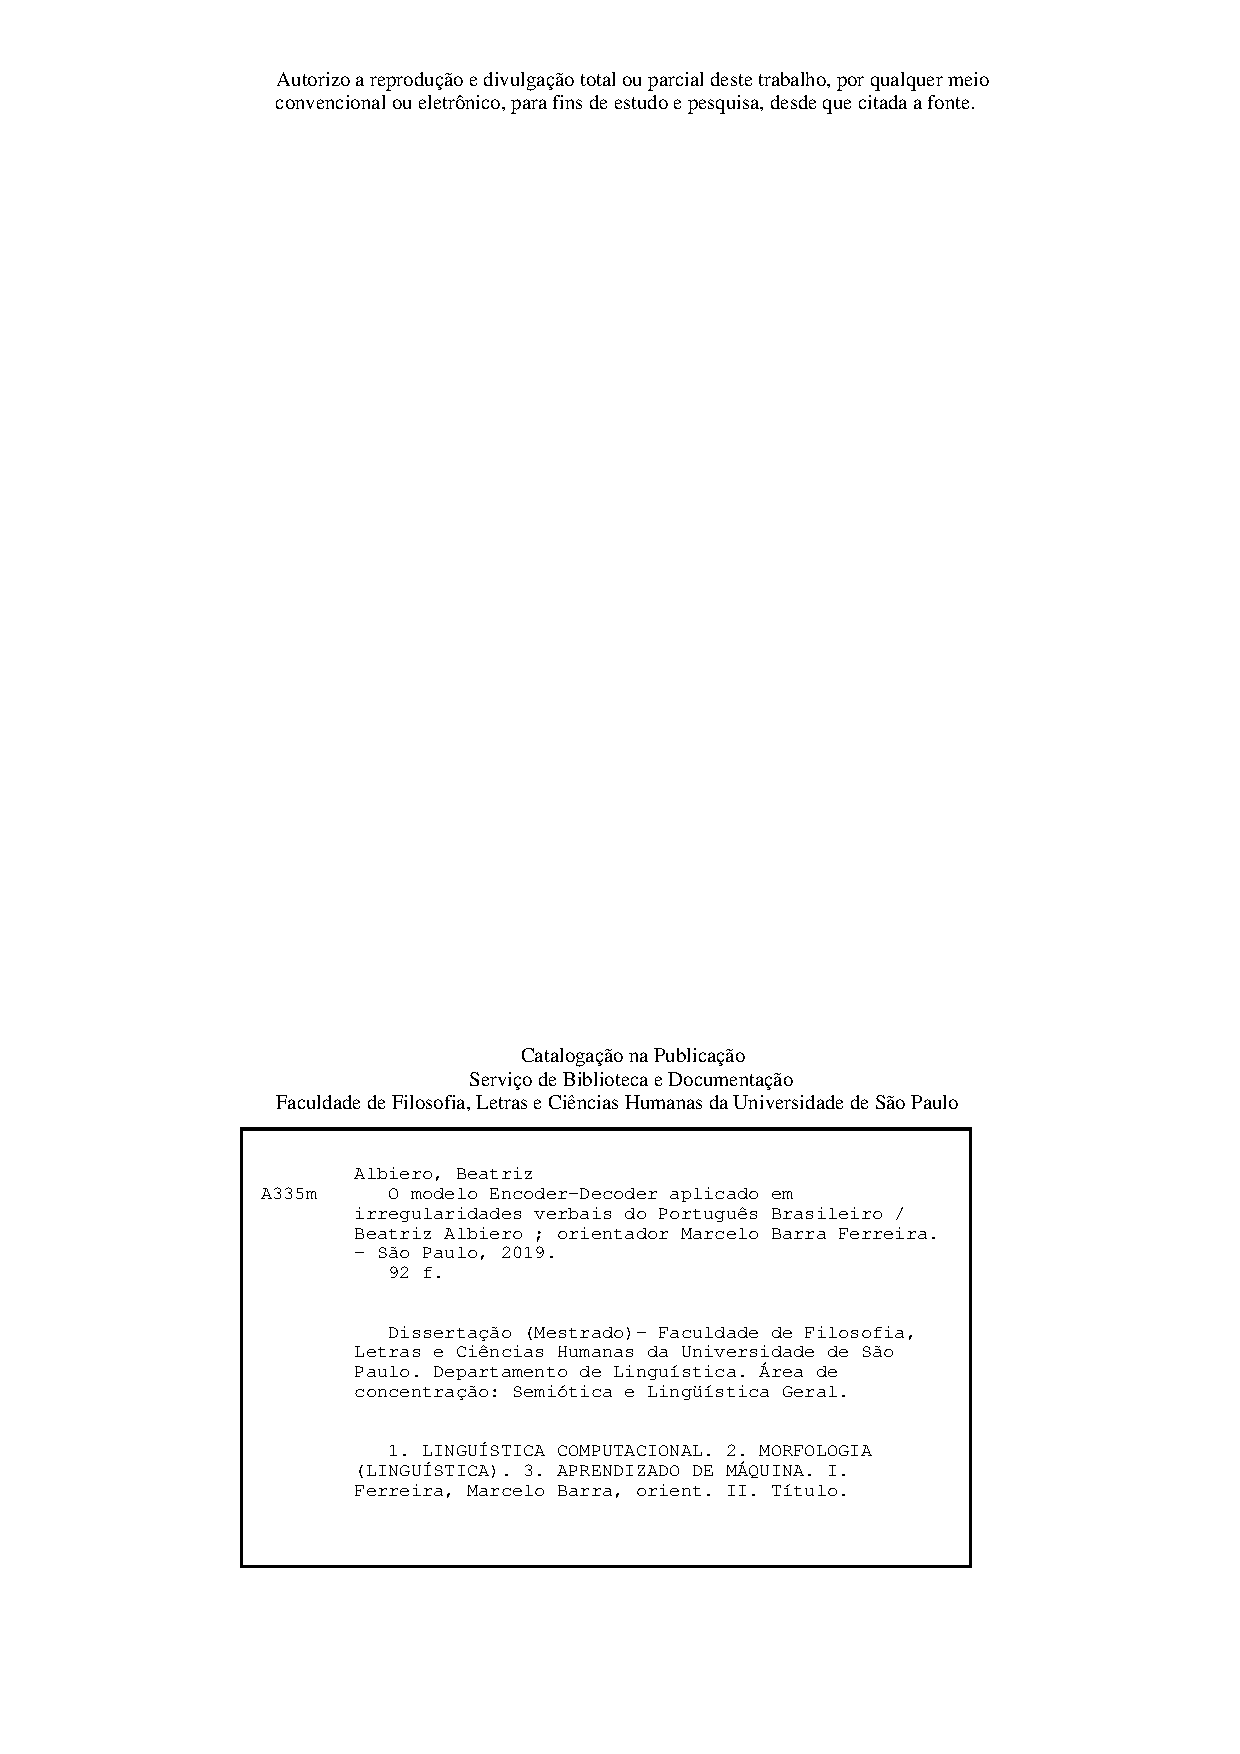
\includepdf[pagecommand={\thispagestyle{plain}},
  pages=-]{fichacatalografica.pdf}
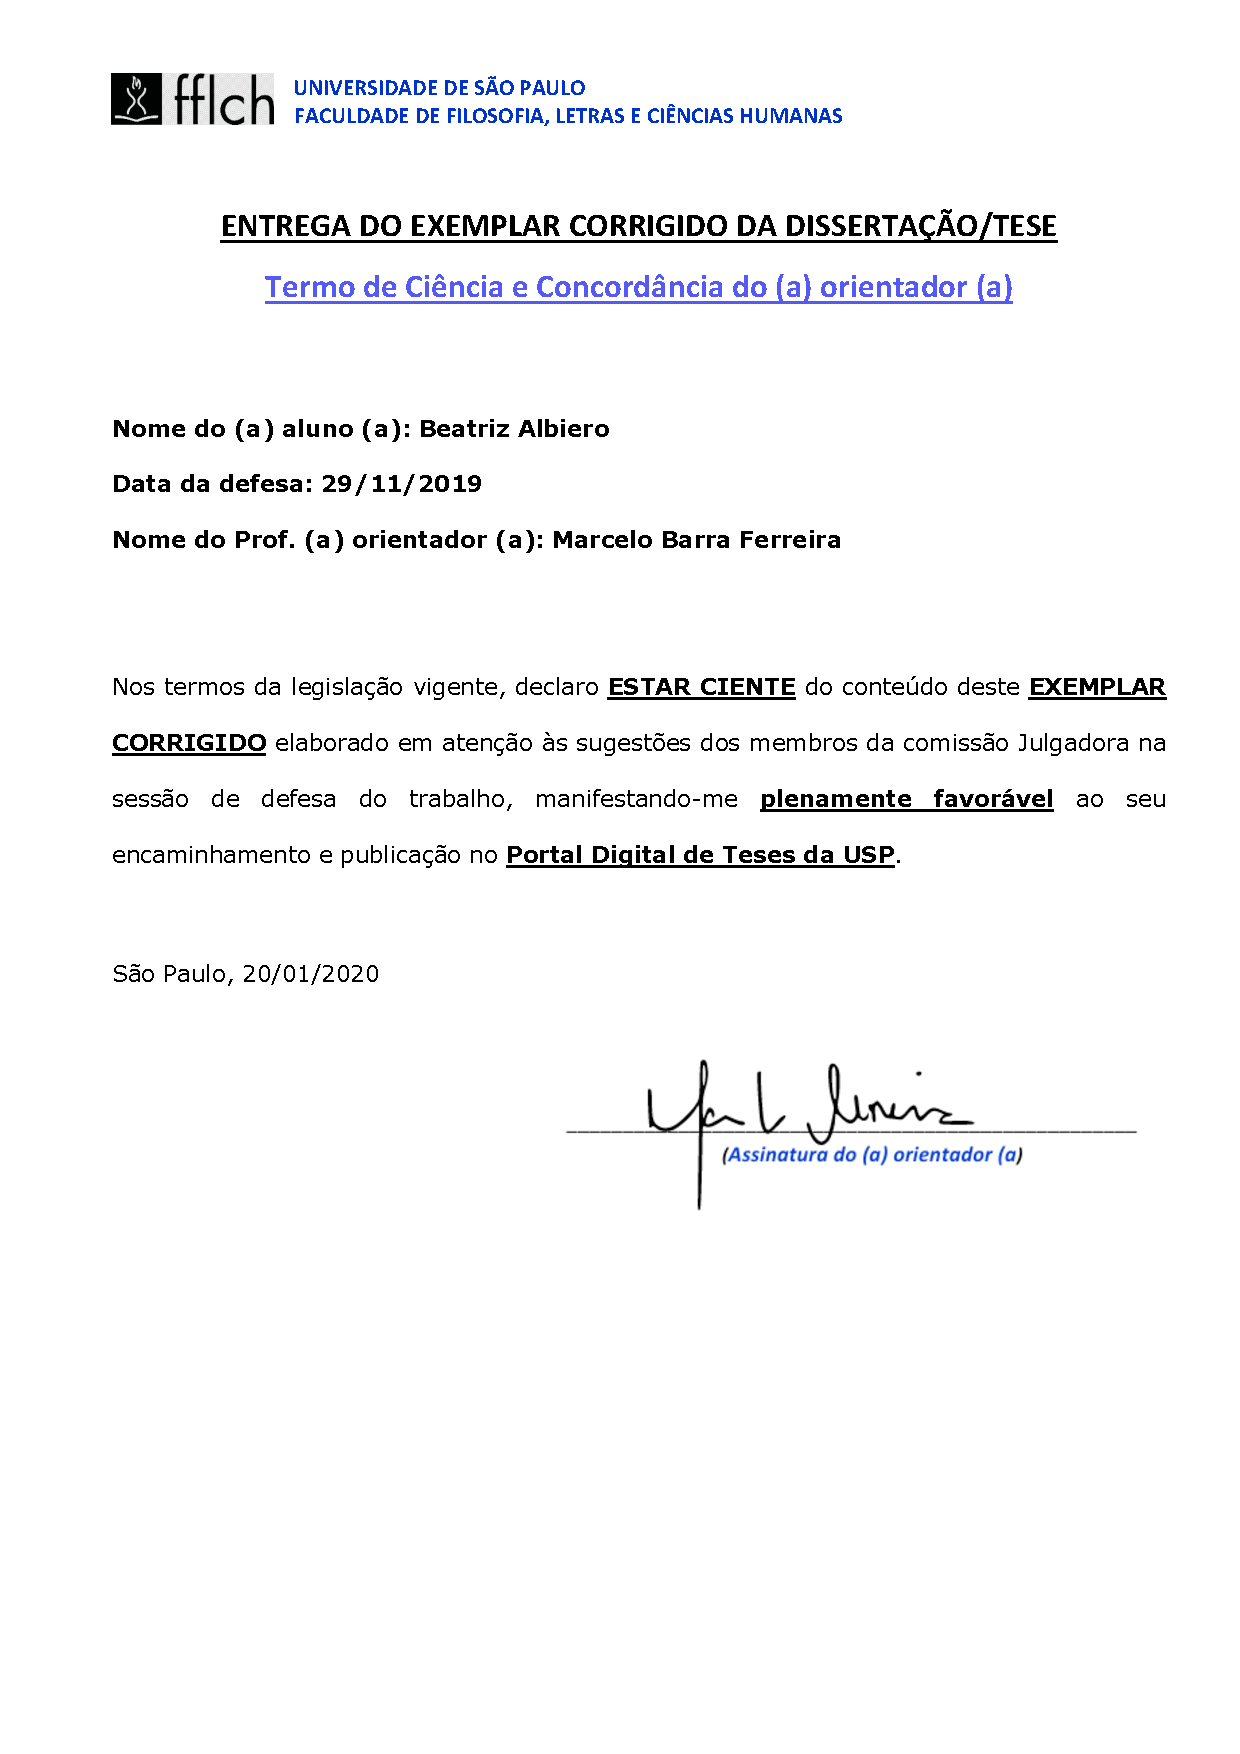
\includepdf[pagecommand={\thispagestyle{plain}},
  pages=-]{termocienciaeditado.pdf}
\begin{folhadeaprovacao}
  \textbf{\Large{Banca Examinadora}}
  \vskip 2cm
    \_\_\_\_\_\_\_\_\_\_\_\_\_\_\_\_\_\_\_
  
    Prof. Dr. Marcelo Barra Ferreira
    
    (USP) Presidente
    \vskip 2cm
    
    \_\_\_\_\_\_\_\_\_\_\_\_\_\_\_\_\_\_\_
    
    Profa. Dra. Livy Maria Real Coelho
    
    Membro Titular
    \vskip 2cm
    
    \_\_\_\_\_\_\_\_\_\_\_\_\_\_\_\_\_\_\_
      
    Prof. Dr. Marcos Fernando Lopes

    (USP) Membro Titular

    \vskip 2cm
    \_\_\_\_\_\_\_\_\_\_\_\_\_\_\_\_\_\_\_
    

    Prof. Dr. Pablo Picasso Feliciano de Faria
    
    (UNICAMP) Membro Titular
 
  
    

\end{folhadeaprovacao}
% ---------------------------------------------------------------------------- %
% Dedicatória
\newenvironment{dedication}
  {%\clearpage           % we want a new page          %% I commented this
   \thispagestyle{empty}% no header and footer
   \vspace*{\stretch{10}}% some space at the top
   \itshape             % the text is in italics
   \raggedleft          % flush to the right margin
  }
  {\par % end the paragraph
   \vspace{\stretch{2}} % space at bottom is three times that at the top
   \clearpage           % finish off the page
  }

 \frontmatter              %% better to use this in book class
 \chapter{}
  \begin{dedication}
    Em memória de Valéria. 
    
    Mãe, amiga, querida. 
    \par   %% or a blank line
    \vspace{2\baselineskip}
    Ao meu pai André, que me deu a maior força 
    
    para começar, continuar e concluir este trabalho.
    
  \end{dedication}

% ---------------------------------------------------------------------------- %
% Agradecimentos

\chapter*{Agradecimentos}
\pagenumbering{gobble}

Posso dizer que eu tive ao meu lado pessoas muito importantes que me ajudaram a passar pela experiência do mestrado de forma incrível. Foram muitos desafios e aprendizados, e sem as pessoas listadas a seguir, certamente esse processo não teria sido tão produtivo. 

Primeiramente, agradeço à minha família, que me apoiou e incentivou nos meus estudos desde sempre. À minha mãe Valéria, que apesar de não ter tido a oportunidade de acompanhar essa fase da minha vida, observa de longe e se faz presente a cada passo que dou. Não sinto saudades, pois sinto que está comigo sempre. Ao meu pai André, meus avós Astrid e Norberto e aos meus irmãos Fábio e Juliana, pelo amor, carinho e cuidado.

Sou muito grata também ao meu orientador Marcelo Barra Ferreira. Tenho a sorte de poder dizer que a minha experiência no mestrado foi muito positiva e enriquecedora em um momento muito delicado para a pós-graduação brasileira, e certamente a sua orientação e parceria foi fundamental nesse processo.

Agradeço aos meus amigos e membros do grupo de estudos em linguística computacional da USP (o GLIC), que me ajudaram e inspiraram. Agradecimentos especiais ao meu colega Bruno Guide, que me ajudou diversas vezes com as minhas questões sobre a pós, muito antes da minha pesquisa começar. Também agradeço à Livy pelo seu olhar crítico e curioso sempre. A forma como todos do grupo amam estudar linguística é incrível. Também agradeço ao querido professor Marcos Lopes, cuja participação também foi fundamental para a minha formação acadêmica e para que o meu ingresso no mundo da linguística ocorresse de maneira leve e agradável.

Agradeço também aos meus colegas do Datalab, que me apoiaram e incentivaram durante a execução desta pesquisa. Sinto-me muito privilegiada por ter tido o apoio que eu tive no meu ambiente de trabalho e por todas as oportunidades que me foram concedidas para o meu desenvolvimento acadêmico. Agradecimento especial a Estêvão Uyrá, que contribuiu diretamente na execução desta pesquisa com sugestões valiosíssimas. Também sou muito grata ao professor Renato Vicente por ter me incluído em um time tão genial e criativo, além de todo o apoio na minha formação acadêmica e profissional. Também agradeço aos meus colegas Sami e Ricardo, pela compreensão, pelos conselhos e risadas.

Também não posso deixar de agradecer ao meu colega Felipe Salvatore, doutorando no IME-USP, que me auxiliou com sugestões essenciais para a base computacional desta pesquisa. Às professoras Esmeralda Vailati Negrão e Maria Cristina Altman que me apresentaram ao universo da linguística e me incentivaram a estudar esse assunto com mais profundidade no mestrado.

Finalmente, a todos aqueles que me apoiaram nos momentos mais difíceis, em especial: Maria Teresa Lamberte, Carlos Joventino, Arthur Athayde, Ramon Vilarino, Thaís Dresch, Marina Nagata e Manu Bonfim. 

% ---------------------------------------------------------------------------- %
% Abstract
\chapter*{Resumo}
\pagenumbering{gobble}
\noindent Albiero, B. \textbf{O modelo Encoder-Decoder aplicado em irregularidades verbais do Português Brasileiro}. 
2019.
Dissertação (Mestrado) - Faculdade de Filosofia e Ciências Humanas,
Universidade de São Paulo, São Paulo, 2019.
\\

Inspirada na controversa questão da aquisição de verbos irregulares na língua inglesa (\cite{chomsky:1968},  \cite{Pinker:1988},
\cite{Albright2003RulesVA}, \cite{kirov:2018}), esta pesquisa tem como objetivo estudar a questão da flexão de verbos irregulares do Português Brasileiro sob a ótica do modelo computacional \textit{Encoder-Decoder}. Para tanto, a tarefa proposta ao modelo era a de predizer uma forma verbal flexionada dada uma forma primária (\textit{Radical + Vogal Temática}). O escopo da pesquisa restringiu-se ao estudo do paradigma de 1\aup{a} Pessoa do Singular no Modo Indicativo e Tempo Presente. O modelo utilizado, por sua vez, é um modelo de caráter associativo que pertence ao grupo dos modelos de Redes Neurais Artificiais. Também, fez-se necessária a construção de um \textit{corpus} linguístico composto pelo paradigma selecionado e em seguida transcrito em notação fonética específica para viabilizar a utilização do modelo escolhido. O \textit{corpus} produzido é composto por 423 verbos que foram marcados como pertencendo às famílias de verbos regulares (51\%) ou irregulares (49\%). Ainda, dentro do escopo da família de verbos irregulares, foi possível identificar 15 subgrupos conforme a identificação de diferentes padrões de flexão. A partir da notação fonética utilizada, os verbos puderam ser associados a novas representações que englobavam informações relativas aos traços fonéticos presentes. Assim, o modelo proposto tenta predizer as formas flexionadas a partir da identificação das relações fonéticas envolvidas durante o processo de flexão. O modelo apresentado foi submetido a múltiplos treinamentos e testes e apresentou uma acurácia média de 13.55\%, mas chegou a acertar 17\% em um dos experimentos. Considerando a segmentação entre verbos regulares e irregulares, o modelo performou melhor na classe dos regulares. Entretanto, considerando-se todas as 16 classes individualmente (15 irregulares + 1 regular), pôde-se observar que as duas primeiras classes em que o modelo performou melhor eram classes irregulares, deixando a classe regular como a terceira com os melhores resultados.

\\
 \textbf{Palavras-chave:}
morfologia verbal, aprendizagem de máquina, conexionismo.

\chapter*{Abstract}
\pagenumbering{gobble}
\noindent Albiero, B. \textbf{The Encoder-Decoder Model Applied to Brazilian-Portuguese Verbal Irregularities}. 
2019.
Dissertação (Mestrado) - Faculdade de Filosofia e Ciências Humanas,
Universidade de São Paulo, São Paulo, 2019.
\\

Inspired by the controversial debate about the acquisition of irregular verbs in Englishlanguage (\cite{chomsky:1968}, \cite{Pinker:1988},
\cite{Albright2003RulesVA}, \cite{kirov:2018}), this research aims to study the inflection process of irregular verbs in Portuguese through the perspective of the computational model \textit{Encoder-Decoder}. To do this, we proposed the task of predicting an inflected verbal form given a primary form (\textit{Stem + Thematic Vowel}). The scope of the research was restricted to the study of the singular first-person paradigm in the indicative mood and present tense. The model, in turn, is an associative model that belongs to the group of Artificial Neural Networks models. Also, it was necessary to construct a linguistic \textit{corpus} composed by the chosen paradigm and then transcribe it into a specific phonetic notation to enable the usage of the chosen model. The resulting \textit{corpus} consists of 423 verbs that were marked as belonging to either regular (51\%) or irregular (49\%) verb families. Moreover, within the scope of irregular verbs, it was possible to identify 15 subgroups through the identification of inflection patterns. Through the phonetic notation provided, verbs could be associated with new representations that included information related to the phonetic features. Thus, the proposed model attempts to predict inflected forms by identifying the involved phonetic relationships during the inflection process. The model was submitted to multiple trainings and tests and presented an average accuracy of 13.55\%, but it got to 17\% in one of the experiments. Considering the segmentation between regular and irregular verbs, the model performed better among the regular class. However, considering all 16 classes individually (15 irregular + 1 regular), it was observed that the first two classes in which the model performed best were irregular classes, leaving the regular class with the third place.

\textbf{Key-words:}
verbal morphology, machine learning, connectionism.

\tableofcontents
\pagestyle{fancy}
\onehalfspacing            % espaçamento um e meio
\mainmatter
\pagenumbering{arabic}
\chapter*{Introdução}
\addcontentsline{toc}{chapter}{Introdução}

Inspirada no controverso tema da aquisição de verbos irregulares na língua inglesa
(\cite{Pinker:1999}, \cite{chomsky:1968},  \cite{Pinker:1988}, \cite{rumelhart:1986}), esta pesquisa tem como objetivo estudar o processo de flexão de verbos irregulares do Português Brasileiro fazendo uso de um modelo computacional conhecido como \textit{Encoder-Decoder} (\cite{enc-dec:2014}).

A controvérsia em torno do processo de aprendizado de verbos irregulares teve início na década de 60, tendo sido explorada por pesquisadores de diversas áreas (linguistas, psicólogos, neurocientistas, cientistas da computação, entre outros). No Cap. \ref{ch:01} deste trabalho, serão apresentadas as origens e motivações da discussão, bem como os principais pesquisadores envolvidos e hipóteses levantadas. Além disso, será introduzida uma categoria de modelos computacionais associativos conhecida como Rede Neural Artificial, do qual o modelo \textit{Encoder-Decoder} faz parte. Em seguida, na primeira parte da seção de motivação (Seç. \ref{sec:motivation}) serão apontadas algumas especificidades gramaticais da língua portuguesa que podem dificultar o processo de aprendizado da flexão irregular. Na segunda parte da seção, serão apresentados alguns trabalhos computacionais que se seguiram nos anos subsequentes em resposta à discussão estabelecida. 

Após a exposição dos diferentes trabalhos desenvolvidos, ficará evidente a razão pela qual tal tema chamou a atenção de tantas áreas distintas. Ademais, veremos que o problema da flexão de verbos irregulares tornou-se um desafio computacional para além dos problemas linguísticos ou cognitivos em questão, de modo que muitas pesquisas subsequentes acabaram se distanciando do debate linguístico e focando nos aspectos matemáticos que viabilizariam o aprendizado artificial. A presente pesquisa também dará continuidade a esse aspecto computacional do problema e não terá como objetivo assumir qualquer posição em torno dos aspectos cognitivos do debate. Desse modo, avaliaremos o uso do modelo \textit{Encoder-Decoder} a partir de um ponto de vista prático de acordo com a sua performance na tarefa proposta e em comparação a outros modelos computacionais já apresentados em outras pesquisas.

Para a realização do objetivo proposto, primeiramente foi necessário o desenvolvimento de um corpus linguístico específico para a tarefa. O corpus resultante apresenta-se completo no Apêndice (\ref{ap:corpus}), mas será discutido em detalhes no Cap. \ref{ch:02}, na Seç \ref{sec:corpus}. Ainda nesse capítulo, veremos a importância da aplicação de tratamentos de pré-processamento adequados nas unidades do corpus para a viabilização do aprendizado pretendido. Para tanto, revisitaremos um algoritmo de pré-processamento proposto em uma pesquisa anterior, realizada por \cite{rumelhart:1986}. Em seguida, apresentaremos o algoritmo de pré-processamento desenvolvido nesta pesquisa.

O Capítulo \ref{ch:03} introduzirá conceitos básicos sobre o tema de \textit{Aprendizado de Máquina} e em seguida apresentará uma introdução aos modelos de Redes Neurais Artificiais. Além disso, abordaremos os conceitos de \textit{Modelo de Linguagem} e de arquiteturas de \textit{Redes Neurais Recorrentes} - assuntos imprescindíveis para o entendimento do modelo em destaque desta pesquisa, o \textit{Encoder-Decoder}. Feitas as devidas introduções, estaremos prontos para a apresentação do modelo \textit{Encoder-Decoder} no Capítulo \ref{ch:05}.  

O Capítulo \ref{ch:07}, por sua vez, apresentará e discutirá os resultados obtidos. Nele veremos as configurações escolhidas para a definição do modelo e as métricas utilizadas para a avaliação do mesmo. Analisaremos também os diferentes erros observados e procuraremos por possíveis explicações para os resultados obtidos. 

Para concluir, o Capítulo \ref{ch:08} exibirá um resumo dos assuntos tratados nesta pesquisa e também apontará sugestões para pesquisas futuras sobre o assunto.





\fancyhead[RE,LO]{\thesection}
\chapter{Introdução}
\label{ch:01}

A questão do aprendizado infantil, referente ao processo de flexão de verbos irregulares na língua inglesa, está certamente entre um dos temas de debate mais controversos %entre as principais correntes teóricas no estudo da 
do campo da Linguística (Pinker, \citeyear{Pinker:1999}). O cerne do debate está na exata caracterização dos mecanismos que possibilitam que um falante seja capaz de relacionar um verbo na forma não flexionada (\textit{walk}, por exemplo) à sua forma flexionada no \textit{Simple Past} (\textit{walked}).

Os verbos no tempo passado do inglês podem ser subdivididos em uma variedade de famílias. Um primeiro grupo é a forma aceita como a \textit{regular}, cuja forma ortográfica corresponde à aplicação da regra \textit{\text{stem} + ed}, como em \textit{walk}. %Entretanto, sob uma perspectiva fonológica, ainda é possível dividir esse grupo em três menores seguindo as variações possíveis do segmento \textit{ed}: (i) [-\textsci d], (ii) [-d] e (iii) [-t]. Em (i), observa-se que o segmento [-\textsci d] é utilizado sempre nos casos em que o último fonema do \textit{stem} for um [t] ou [d], como por exemplo o verbo \textit{pad} $\rightarrow$ \textit{padded} ([p\ae d] $\rightarrow$ [p\ae d\textsci d]). A situação (ii) é utilizada sempre que último fonema do \textit{stem} for uma vogal ou uma consoante sonora, como por exemplo em \textit{drag}$\rightarrow$ dragged ([dr\ae g]) $\rightarrow$ [dr\ae gd] ou show$\rightarrow$ showed ([\textesh o\textupsilon]$\rightarrow$[\textesh o\textupsilon d]). Por sua vez, o caso (iii) é aplicado sempre após uma consoante surda (\textit{sack}$\rightarrow$ sacked ([s\ae k] $\rightarrow$ [s\ae kt]). 
% ocorrendo não somente a formação de um padrão regular (que ortograficamente corresponde à composição verbo + \textit{ed}), mas também à formação de subgrupos de verbos irregulares, como por exemplo:
Dentre os verbos irregulares, estes podem ser considerados supletivos, como por exemplo \textit{go} $\rightarrow$ \textit{went}, ou podem se conglomerar seguindo padrões fonéticos de flexão similares (\cite{Nelson:2010}):

\begin{enumerate}
    \item blow – blew, grow – grew, know – knew, throw – threw
    \item bear – bore, swear – swore, tear – tore, wear – wore
    \item drink – drank, shrink – shrank, sink – sank, stink – stank 
\end{enumerate}

É possível pensar que o aprendizado de tais padrões dependeria de uma memorização caso a caso. No entanto, a pesquisa de \cite{Bybee:1983} mostra um estudo psicolinguístico em que indivíduos são apresentados a diversos verbos inventados (hipoteticamente em uma forma não flexionada). A pesquisa revelou que, ao invés de aplicarem sistematicamente a regra regular (verbo + \textit{ed}), os indivíduos apresentaram tendências à alocação de alguns verbos em alguns subgrupos irregulares. % um estudo psicolinguístico conduzido a partir da  verbos inventados revelou que os indivíduos apresentam tendências com relação à alocação dos verbos também em grupos de verbos irregulares, ao invés de sistematicamente aplicar a regra regular ( + \textit{ed}). 
Por exemplo, para o verbo inventado “\textit{spling}”, a maioria dos indivíduos optou pela forma “\textit{splang}”  ou “\textit{splung}”. Este exemplo contradiz a ideia de que os falantes poderiam estar apenas reproduzindo formas memorizadas e sugere que eles estejam ativamente identificando padrões, e mais: possuem uma intuição natural sobre a adequabilidade da alocação de um verbo a um grupo de verbos ou a outro. 

A partir do exemplo dado, é razoável deduzir que a motivação por de trás de tais tendências ocorra a partir das similaridades entre as unidades fonéticas dos verbos inventados e os verbos reais que já apresentam uma flexão de caráter irregular. Entretanto, as circunstâncias que levam à aquisição dessa \textit{intuição} linguística são indeterminadas. Por um lado, faz sentido dizer que para que um ser humano seja capaz de introduzir-se ao mundo dos falantes, é necessário que ele seja dotado de algumas pré-disposições para tal, caso contrário seria possível ensinar essa forma de comunicação para outras espécies. Em contrapartida, estudos mostram que crianças privadas do contato com uma sociedade falante se tornam permanentemente incapazes de dominar integralmente a gramática de uma língua (\cite{Pinker:languageinstinct}), o que nos leva a concluir que a experiência das crianças com a sociedade, assim como as suas próprias pré-disposições genéticas são ambas parcialmente responsáveis pelo processo de desenvolvimento da linguagem. A dificuldade, está portanto, na tentativa de se quantificar, delimitar e apontar os conhecimentos adquiridos a partir do contato cultural, bem como os conhecimentos linguísticos ditos \textit{inatos}. É, portanto, em torno desta questão que tem início o debate a respeito do aprendizado dos verbos irregulares da língua Inglesa.

%https://plato.stanford.edu/entries/rationalism-empiricism/


De um lado do debate, encontra-se a teoria da Fonologia Gerativa de Chomsky e Halle (\citeyear{chomsky:1968}). Nesta teoria, os indivíduos seriam portadores de um dispositivo de aquisição de linguagem (\textit{LAD} - Language Acquisition Device) responsável pela \textit{formulação} e \textit{manipulação} de estruturas fonológicas abstratas em um sistema intrincado de regras. De modo simplificado, a teoria propõe que o falante seja capaz de identificar e formular regras intuitivamente para dar conta do aprendizado das formas irregulares da língua. Um exemplo disso é a família dos verbos terminados em “-ind”.

\begin{center}
bind – bound, find – found, grind – ground, wind – wound
\end{center}

Vemos que, de modo simplificado, pode-se propor uma regra baseada em uma gramática sensível a contextos (Context-Sensitive Grammar (CSG) (ref)) 
%verificar essa formula fonetica

\begin{center}
a\textsci $\rightarrow$ a\textupsilon / \textbf{X}  \_\_nd]+past
\end{center}

A regra proposta sugere que o segmento [a\textsci] se transforma em [a\textupsilon] quando terminado em [nd] e flexionado para o passado. O símbolo \_\_ representa o local aonde ocorre tal transformação e \textbf{X} representa uma unidade fonológica arbitrária. 

Em outras palavras, pode-se dizer que o conhecimento dito \textit{inato} defendido por Chomsky e Halle refere-se a uma certa capacidade cognitiva de formulação de regras a partir da identificação de alguns elementos fundamentais (como por exemplo os elementos apontados na regra proposta). Uma estrutura como essa permitiria ao falante construir generalizações e, eventualmente, abstrair as regras fonológicas de sua língua. \\

Do outro lado do debate, os pesquisadores \cite{rumelhart:1986} confrontam a teoria anterior ao argumentar que comportamentos de caráter regrado podem ser reproduzidos por mecanismos que não dependam de nenhuma manipulação simbólica. Ao invés disso, os pesquisadores sugerem que os mecanismos envolvidos no processo de flexão verbal possam ser construídos de tal forma que a sua performance possa ser descrita através de regras, mas que as regras em si não estejam representadas explicitamente em nenhuma parte do processo. Para sustentar essa ideia, \cite{rumelhart:1986} apresentam um modelo computacional baseado em padrões associativos que não fazem uso de construções com regras desse tipo. Posteriormente, o modelo construído foi fundamental para o surgimento de uma nova escola dentro das ciências cognitivas: o conexionismo.\\

\definecolor{blue}{RGB}{159, 192, 176}
\definecolor{green}{RGB}{160, 227, 127}
\definecolor{orange}{RGB}{243, 188, 125}
\definecolor{red}{RGB}{253, 123, 84}
\definecolor{nephritis}{RGB}{39, 174, 96}
\definecolor{emerald}{RGB}{46, 204, 113}
\definecolor{turquoise}{RGB}{39, 174, 96}
\definecolor{green-sea}{RGB}{22, 160, 133}
\definecolor{purple}{RGB}{181, 124, 215}
% Tikzstyles for Computation Graphs

% nodes
\tikzstyle{noop} = [circle, draw=none, fill=red, minimum size = 10pt]
\tikzstyle{op} = [circle, draw=red, line width=1.5pt, fill=red!70, text=black, text centered, font=\bf \normalsize, minimum size = 25pt]

\tikzstyle{opintense} = [circle, draw=red, line width=1.5pt, fill=red!150, text=black, text centered, font=\bf \normalsize, minimum size = 25pt]


%new style
\tikzstyle{gp} = [circle, draw=red, line width=4pt, text=black, text centered, font=\bf \normalsize, minimum size = 4.cm]

\tikzstyle{box} = [rectangle, draw=red, line width=1.5pt, fill=red!70, text=black, align=center, font=\bf \normalsize, minimum size = 45pt]

\tikzstyle{box2} = [rectangle, draw=black, line width=0.9pt, text=black, align=center, font=\bf \normalsize, minimum size = 20pt]

\tikzstyle{box3} = [rectangle, draw=black, line width=0.9pt, fill=black, text=black, align=center, font=\bf \normalsize, minimum size = 20pt]

\tikzstyle{state} = [circle, draw=blue, line width=1.5pt, fill=blue!70, text=black, text centered, font=\bf \normalsize, minimum size = 25pt]

\tikzstyle{output} = [circle, draw=purple, line width=1.5pt, fill=purple!70, text=black, text centered, font=\bf \normalsize, minimum size = 25pt]


\tikzstyle{gradient} = [circle, draw=nephritis, line width=1.5pt, fill=nephritis!60, text=black, text centered, font=\bf \normalsize, minimum size = 25pt]
\tikzstyle{textonly} = [draw=none, fill=none, text centered, font=\bf \normalsize]
\tikzstyle{boxtextonly} = [draw=none, fill=none, align=center, font=\bf \normalsize]

\tikzstyle{normal} = [circle, draw=black, line width=1.0pt, fill=none, text=black, text centered, font=\bf \normalsize, minimum size = 20pt]


% edges
\tikzstyle{tedge}  = [draw, thick, >=latex, ->]
\tikzstyle{tedge_dashed}  = [draw, thick, >=latex, ->, dashed]
\tikzstyle{nedge}  = [draw, thick, >=latex]
\tikzstyle{nedge_dashed}  = [draw, thick, >=latex, dashed]


% namedscope
\tikzstyle{namedscope} = [circle, draw=orange, line width=1.5pt, fill=orange!60, align=center, inner sep=0pt]
\begin{figure}[ht!]
\centering

\scalebox{1.0}{
\begin{tikzpicture}[auto]

% operations =========
% phon features 1
\node[textonly] (1pho1) {int-vogal-int};

% Legenda
\node[textonly, above=10pt of 1pho1] (leg1) {Unidades de Input};


% FNN input
\node[normal, right=5pt of 1pho1] (x1) {};
\node[normal, below=25pt of x1] (x2) {};
\node[normal, below=25pt of x2] (x3) {};
\node[normal, below=25pt of x3] (x4) {};
\node[normal, below=25pt of x4] (x5) {};
\node[normal, below=25pt of x5] (x6) {};

% FNN output
\node[normal, right=45pt of x1] (y1) {};
\node[normal, right=45pt of x2] (y2) {};
\node[normal, right=45pt of x3] (y3) {};
\node[normal, right=45pt of x4] (y4) {};
\node[normal, right=45pt of x5] (y5) {};
\node[normal, right=45pt of x6] (y6) {};

% phon features 2
\node[textonly, right=5pt of y1] (2pho1) {int-vogal-int};
\node[textonly, above=10pt of 2pho1] (leg2) {Unidades de Output};
\node[textonly, left=25pt of x2] (1pho2) {anterior-nasal-posterior};
\node[textonly, right=25pt of y2] (2pho2) {anterior-nasal-posterior};
\node[textonly, left=25pt of x3] (3pho1) {...};
\node[textonly, right=25pt of y3] (1pho3) {...};
\node[textonly, left=25pt of x4] (4pho1) {nasal-cont-ocl};
\node[textonly, right=25pt of y4] (1pho4) {nasal-cont-ocl};
\node[textonly, left=25pt of x5] (5pho1) {médio-cont-baixa};
\node[textonly, right=25pt of y5] (1pho5) {médio-cont-baixa};
\node[textonly, left=25pt of x6] (6pho1) {vogal-fric-\#};
\node[textonly, right=25pt of y6] (1pho6) {vogal-fric-\#};
% edges FNN
\path[nedge] (x1) -- (y1);
\path[nedge] (x1) -- (y2);
\path[nedge] (x1) -- (y3);
\path[nedge] (x1) -- (y4);
\path[nedge] (x1) -- (y5);
\path[nedge] (x1) -- (y6);
\path[nedge] (x2) -- (y1);
\path[nedge] (x2) -- (y2);
\path[nedge] (x2) -- (y3);
\path[nedge] (x2) -- (y4);
\path[nedge] (x2) -- (y5);
\path[nedge] (x2) -- (y6);
\path[nedge] (x3) -- (y1);
\path[nedge] (x3) -- (y2);
\path[nedge] (x3) -- (y3);
\path[nedge] (x3) -- (y4);
\path[nedge] (x3) -- (y5);
\path[nedge] (x3) -- (y6);
\path[nedge] (x4) -- (y1);
\path[nedge] (x4) -- (y2);
\path[nedge] (x4) -- (y3);
\path[nedge] (x4) -- (y4);
\path[nedge] (x4) -- (y5);
\path[nedge] (x4) -- (y6);
\path[nedge] (x5) -- (y1);
\path[nedge] (x5) -- (y2);
\path[nedge] (x5) -- (y3);
\path[nedge] (x5) -- (y4);
\path[nedge] (x5) -- (y5);
\path[nedge] (x5) -- (y6);
\path[nedge] (x6) -- (y1);
\path[nedge] (x6) -- (y2);
\path[nedge] (x6) -- (y3);
\path[nedge] (x6) -- (y4);
\path[nedge] (x6) -- (y5);
\path[nedge] (x6) -- (y6);


\end{tikzpicture}
}\caption{Esquema da rede neural utilizada pelos pesquisadores Rumelhart e McClelland} 
\label{fig:esquemafdd}
\end{figure}


O modelo desenvolvido foi criado por analogia à estrutura em que se relacionam os neurônios no cérebro. Ele é composto basicamente por uma rede artificial de nódulos interconectados paralelamente (Fig. \ref{fig:esquemafdd}).

A primeira camada de nódulos do modelo é responsável por receber os dados de entrada (os \textit{inputs}), que são os dados referentes aos traços fonéticos distintivos que caracterizam os sons de um verbo não flexionado. Traços fonéticos podem ser caracterizados como propriedades distintivas das unidades fônicas (\cite{paraconhecer:2015}). Tais propriedades podem ser baseadas em critérios acústicos, articulatórios ou perceptuais. Na figura, cada nódulo é apresentado ao lado de uma sequência de três traços. O primeiro nódulo, por exemplo, refere-se à sequência \textbf{int-vogal-int}. Nesse caso, \textbf{int} (uma abreviação para \textit{interrompida}) indica uma propriedade comum entre algumas consoantes, referente à interrupção do fluxo de ar (como no fone [k], por exemplo). Na figura temos ainda \textbf{fric} para fricativas; \textbf{ocl} para oclusivas; vogais; \textbf{nasal} para nasalidade; locais da execução (anterior e posterior); traços de corpo da língua (média, baixa); entre outros. Ainda sobre a camada de \textit{input}, é possível observar que cada nódulo é representado por uma tríade de traços fonéticos. Esta foi uma solução encontrada pelos autores para realizar o mapeamento entre os traços dos verbos da forma não flexionada para o \textit{Past Simple}. Os \textit{inputs} são estruturados dessa forma para contornar a dificuldade de inserção de dados de natureza sequencial e de tamanho variável (como é o caso de um verbo - composto por uma sequência de sons). Cada tríade é uma associação de três traços, cada um referente a um fone. Por exemplo, para o verbo \textit{came} (transcrito em forma fonética pelos autores como \textit{/kAm/}), temos que cada um dos fones possui múltiplos traços. O fone [\textit{k}], por exemplo, é uma consoante interrompida, surda e anterior. Os fones subsequentes também são constituídos a partir de seus respectivos traços fonéticos, de modo que cada traço esteja associado a cada fone da sequência (Tabela \ref{tab:trigrams}). O tema dos traços fonéticos utilizados, bem como todo o esquema de pré-processamento utilizado pelos autores será abordado em maior profundidade no Cap. \ref{ch:02}.

\begin{table}[H]
\begin{center}
\begin{tabular}{ccc}
k                    & A                    & m                    \\ \hline
surda                & longa                & nasal                \\
interrompida         & vogal                & interrompida         \\
anterior             & baixa                & posterior            \\
consoante            & posterior            & consoante            \\
\multicolumn{1}{l}{} & \multicolumn{1}{l}{} & \multicolumn{1}{l}{}
\end{tabular}
\caption{Tríades de Traços Fonéticos Utilizados nos \textit{Inputs} do modelo de Rumelhart e McClelland}
\label{tab:trigrams}
\end{center}
\end{table}

Em seguida, o \textit{input} recebido é passado adiante para a próxima camada através de uma rede de conexões. A segunda camada é uma camada de resposta (\textit{output}) que tem como objetivo retornar dados referentes aos traços que caracterizam os sons do mesmo verbo fornecido no \textit{input}, porém no tempo passado. Concluída esta etapa, os dados de saída obtidos deverão ser então comparados à forma correta do verbo no tempo passado, através de uma espécie de gabarito, usualmente conhecido como \textit{alvo} ou também \textit{target} (Fig.\ref{fig:gabarito}). Feita essa comparação, é possível alterar a rede de conexões entre as camadas de \textit{input} e \textit{output} de modo a fortalecer (ou enfraquecer) as mesmas para atingir o objetivo proposto. Antes da primeira comparação, a rede é inicializada com conexões aleatórias. Conforme o número de comparações aumenta, a tendência é que as atualizações realizadas tenham servido como um aprendizado (uma espécie de \textit{treinamento}) e permitam que o modelo seja utilizado para encontrar os padrões de flexão dos verbos.

\definecolor{blue}{RGB}{159, 192, 176}
\definecolor{green}{RGB}{160, 227, 127}
\definecolor{orange}{RGB}{243, 188, 125}
\definecolor{red}{RGB}{253, 123, 84}
\definecolor{nephritis}{RGB}{39, 174, 96}
\definecolor{emerald}{RGB}{46, 204, 113}
\definecolor{turquoise}{RGB}{39, 174, 96}
\definecolor{green-sea}{RGB}{22, 160, 133}
\definecolor{purple}{RGB}{181, 124, 215}
% Tikzstyles for Computation Graphs

% nodes
\tikzstyle{noop} = [circle, draw=none, fill=red, minimum size = 10pt]
\tikzstyle{op} = [circle, draw=red, line width=1.5pt, fill=red!70, text=black, text centered, font=\bf \normalsize, minimum size = 25pt]

\tikzstyle{opintense} = [circle, draw=red, line width=1.5pt, fill=red!150, text=black, text centered, font=\bf \normalsize, minimum size = 25pt]


%new style
\tikzstyle{gp} = [circle, draw=red, line width=4pt, text=black, text centered, font=\bf \normalsize, minimum size = 4.cm]

\tikzstyle{box} = [rectangle, draw=red, line width=1.5pt, fill=red!70, text=black, align=center, font=\bf \normalsize, minimum size = 45pt]

\tikzstyle{box2} = [rectangle, draw=black, line width=0.9pt, text=black, align=center, font=\bf \normalsize, minimum size = 20pt]

\tikzstyle{box3} = [rectangle, draw=black, line width=0.9pt, fill=black, text=black, align=center, font=\bf \normalsize, minimum size = 20pt]

\tikzstyle{state} = [circle, draw=blue, line width=1.5pt, fill=blue!70, text=black, text centered, font=\bf \normalsize, minimum size = 25pt]

\tikzstyle{output} = [circle, draw=purple, line width=1.5pt, fill=purple!70, text=black, text centered, font=\bf \normalsize, minimum size = 25pt]


\tikzstyle{gradient} = [circle, draw=nephritis, line width=1.5pt, fill=nephritis!60, text=black, text centered, font=\bf \normalsize, minimum size = 25pt]
\tikzstyle{textonly} = [draw=none, fill=none, text centered, font=\bf \normalsize]
\tikzstyle{boxtextonly} = [draw=none, fill=none, align=center, font=\bf \normalsize]

\tikzstyle{normal} = [circle, draw=black, line width=1.0pt, fill=none, text=black, text centered, font=\bf \normalsize, minimum size = 20pt]


% edges
\tikzstyle{tedge}  = [draw, thick, >=latex, ->]
\tikzstyle{tedge_dashed}  = [draw, thick, >=latex, ->, dashed]
\tikzstyle{nedge}  = [draw, thick, >=latex]
\tikzstyle{nedge_dashed}  = [draw, thick, >=latex, dashed]


% namedscope
\tikzstyle{namedscope} = [circle, draw=orange, line width=1.5pt, fill=orange!60, align=center, inner sep=0pt]
\begin{figure}[h]
\centering

\scalebox{1.0}{
\begin{tikzpicture}[auto]

% operations =========
% phon features 1
\node[textonly] (out1) {Output};
\node[textonly, right=25pt of out1] (gab) {Alvo};


% FNN output
\node[normal, below=40pt of out1] (x1) {$y_{1}$};
\node[normal, below=35pt of x1] (x2) {$y_{2}$};
\node[normal, below=35pt of x2] (x3) {$y_{3}$};

% from input
\node[text, left=45pt of x1] (in1) {};
\node[text, left=45pt of x2] (in2) {};
\node[text, left=45pt of x3] (in3) {};


% comparison
\node[text, right=31pt of x1] (nada1) {};
\node[text, below=5pt of nada1] (nada2) {\small{Comparação}};
\node[text, below=10pt of out1] (update) {\small{Atualização}};
\node[text, right=31pt of x2] (nada6) {};
\node[text, right=31pt of x3] (nada7) {};

\node[text, left=31pt of x1] (nada3) {};
\node[text, left=31pt of x2] (nada4) {};
\node[text, left=31pt of x3] (nada5) {};


% FNN target
\node[normal, right=65pt of x1] (y1) {$\hat{y_{1}}$};
\node[normal, right=65pt of x2] (y2) {$\hat{y_{2}}$};
\node[normal, right=65pt of x3] (y3) {$\hat{y_{2}}$};
\node[text, below=15pt of x3] (nada) {};



% edges FNN
\path[arrows_dashed] (x1) -- (y1);
\path[arrows_dashed] (x2) -- (y2);
\path[arrows_dashed] (x3) -- (y3);

\draw[arrows_dashed, ->] (nada1) to [out=135,in=115] (nada3);
\draw[arrows_dashed, ->] (nada6) to [out=135,in=115] (nada4);
\draw[arrows_dashed, ->] (nada7) to [out=135,in=115] (nada5);

\path[tedge] (in1) -- (x1);
\path[tedge] (in2) -- (x1);
\path[tedge] (in3) -- (x1);

\path[tedge] (in1) -- (x2);
\path[tedge] (in2) -- (x2);
\path[tedge] (in3) -- (x2);

\path[tedge] (in1) -- (x3);
\path[tedge] (in2) -- (x3);
\path[tedge] (in3) -- (x3);



\end{tikzpicture}
}\caption{Comparações entre o \textit{Output} e o \textit{Target}} 
\label{fig:gabarito}
\end{figure}

Para realizar o treinamento, \cite{rumelhart:1986} introduzem 420 verbos no modelo repetidamente (200 vezes cada um, 84.000 inserções no total).  Após o treinamento, o modelo foi capaz de prever corretamente todos os 420 verbos inseridos. Além disso, em um novo conjunto com 86 verbos desconhecidos, acertou cerca de 3/4 dos verbos regulares presentes. Dentre os novos verbos irregulares, cometeu erros interessantes de \textit{regularização} (como \textit{catched} (ao invés de caught) e \textit{digged} (ao invés de dug)). %(\cite{Pinker:1999}).  

Além desses resultados, \cite{rumelhart:1986} relatam que o processo de aprendizado do modelo apresentou um fenômeno interessante, reproduzindo um desempenho similar a comportamentos observáveis em crianças durante a fase de aquisição: a Curva de Desenvolvimento em U (U-shaped Development, \cite{marcus:1992}). A Curva de Desenvolvimento em U basicamente se refere a um processo de aprendizado que ocorre em três estágios: \\

(i) inicialmente, crianças aprendem a flexionar verbos corretamente (\textit{come}$\rightarrow$\textit{came});

(ii) em seguida passam por um processo de \textit{super-regularização} (em que produzem formas como \textit{comed}), conforme são capazes de assimilar uma quantidade maior de verbos e compreender que existe uma fórmula genérica que funciona quase sempre;

(iii) por fim, elas entendem (intuitivamente) que a fórmula regular não dá conta de todos os casos e passam a reproduzir corretamente tanto os verbos regulares quanto irregulares. \\


\cite{rumelhart:1986} descrevem como foi possível observar tal comportamento também no modelo computacional desenvolvido.
Na fase inicial do processo de treinamento, o modelo foi alimentado com uma quantidade pequena de verbos, como: \textit{come}, \textit{get}, \textit{give}, \textit{look}, \textit{take}, \textit{go}, \textit{have}, \textit{live} e \textit{feel}. A performance do modelo foi compatível com o primeiro estágio da curva, ou seja, para esses verbos foi capaz de identificar corretamente a forma correspondente no \textit{Simple Past}. Em um segundo momento, o modelo foi alimentado com uma quantidade muito maior de verbos. Nesse estágio é possível verificar que o modelo está passando por um processo de regularização sistemática dos verbos. Ele produziu resultados como: \textit{breaked}, \textit{comed}, \textit{gived}; e também combinações entre padrões regulares e irregulares (ex. \textit{gaved}). 
Após uma série de muitas inserções repetidas, o modelo finalmente foi capaz de responder corretamente a uma quantidade maior de verbos, assim como no último estágio do processo de aprendizado natural. 

Os resultados de \cite{rumelhart:1986} foram capazes de causar bastante alvoroço na comunidade científica da época. Muitos pesquisadores viam o novo modelo como uma completa mudança de paradigma, não apenas na Linguística, mas também como uma nova forma de se estudar aprendizado em geral (\cite{Schneider1987}). 

Apesar disso, \cite{Pinker:1988} dão continuidade ao debate ao apontar uma série de questões pertinentes em que o modelo falhou em explicar. Primeiramente, como o modelo recebe apenas uma representação fonética do verbo como \textit{input}, ele é incapaz de gerar duas respostas diferentes para verbos com sonoridade idêntica (por exemplo \textit{break}$\rightarrow$\textit{broke} e \textit{brake}$\rightarrow$\textit{braked}). Para realizar essas predições corretamente, o modelo precisaria de um módulo adicional para distinguir entre as duas palavras, o que o descaracterizaria como modelo puramente associativo. Em segundo lugar, o modelo é extremamente dependente dos padrões observados durante o treinamento, tendo uma capacidade baixa para generalizações. \cite{Pinker:1999} comenta que o modelo ficou mudo quando alimentado com os verbos \textit{jump}, \textit{pump}, \textit{warm, trail} e \textit{glare} (que dispõem de uma sonoridade razoavelmente incomum). Além disso, o modelo apresentou alguns resultados completamente distorcidos, como: \textit{squat – squakt, tour – toureder} e \textit{mail – membled}; associações inaceitáveis para qualquer falante nativo. 

Com relação ao padrão de aprendizado observado (a Curva de Desenvolvimento em U), \cite{Pinker:1999} explica que esse comportamento foi provocado segundo a forma em que os verbos foram inseridos no modelo durante o treinamento: Rumelhart \& McClelland realizaram o treinamento em partes e controlando a quantidade de repetições de cada lote de verbos. Na primeira parte do treinamento, selecionaram alguns verbos de alta frequência na língua inglesa (muitos deles irregulares), reproduzindo o estágio (i) da curva. Em seguida, treinaram o modelo com esses verbos, reintroduzindo-os múltiplas vezes até que o modelo conseguisse atingir um desempenho razoável nesses verbos. Na sequência introduziram uma quantidade maior de verbos, sendo estes menos frequentes que os anteriores, mas em sua maioria regulares. Dessa forma, o modelo começou a se ajustar para aplicar a regra regular e assim foi possível observar os estágios (ii) e (iii) da curva. Ainda, segundo \cite{pluket:1991}, os estágios de desenvolvimento (i), (ii) e (iii) podem ser considerados parte de um comportamento \textit{macro U-shape}, mas ainda é possível observar a ocorrência de um comportamento \textit{micro U-shape}. \cite{pluket:1991} observam que a reprodução dos verbos irregulares oscila bastante entre flexões corretas e \textit{super-regularizadas}. Eles também notam que estas oscilações ocorrem em proporções diferentes para cada verbo e que crianças raramente “\textit{irregularizam}” verbos regulares (como \textit{ping}$\rightarrow$\textit{pang}), e raramente misturam uma forma irregular com uma regular (fato que ocorreu durante o aprendizado do modelo com \textit{gaved}).

Para concluir, \cite{Pinker:1988} apresentam a formulação de uma nova teoria linguística para tal questão: uma teoria híbrida na qual a fonologia gerativa se aplicaria ao processo de flexão regular e um mecanismo associativo se aplicria ao processo de flexão irregular. Os pesquisadores propõem que as formas regulares sejam computadas a partir de um mecanismo que deve abstrair o radical do verbo e combiná-lo ao sufixo –ed.  Tal mecanismo pode ser aplicado a qualquer palavra, em um processo independente da memória. As formas irregulares, por sua vez, passam por um processo diferente: verbos irregulares precisam passar por um processo de memorização, havendo não somente a associação entre um verbo e outro mas também entre as propriedades (traços fonéticos, rima, stem, núcleo, etc.) de um verbo e de outro, parecido com o que foi proposto por Rumelhart e McClelland.

\section{Motivação}
\label{sec:motivation}

\subsection{Motivação no campo da Linguística}

\subsubsection{Complexidade da Língua Portuguesa}

A morfologia verbal da língua Inglesa é bastante simples, se comparada à Portuguesa. Em primeiro lugar, os verbos do Português se distribuem em três classes módicas (\textit{conjugações}), sendo cada uma destas definida a partir de uma \textit{vogal temática} (\textit{/a/}, \textit{/e/} e \textit{/i/}). Dado um verbo em sua forma infinitiva, por exemplo \textit{Amar}, a vogal temática é a aquela que se encontra entre o morfema lexical do verbo (o radical) e o fone \textit{r}.

\begin{align*}
    \text{Am + a + r}\\
    \text{Radical + VT + r} 
\end{align*}

Com isto, os três possíveis tipos de conjugação são: 1\aup{a} - ar (amar, brigar), 2\aup{a} - er (beber, comer) e 3\aup{a} (rir, descobrir). Na língua Inglesa, essa distinção não existe. 

Outra diferença entre as línguas pode ser observada com relação às pessoais gramaticais das línguas. No Inglês, com exceção do grupo \textit{to be} que apresenta três formas possíveis (considerando o tempo presente): (i) I \textit{am}, (ii) he/she/it \textit{is} e (iii) they \textit{are}; o restante dos verbos apresenta apenas duas: a forma base para \textit{I, We} e \textit{They} (por exemplo, \textit{walk}) e base + s para \textit{he/she/it }(\textit{walks}). No \textit{Past Simple} apresenta maior número de formas também apenas para o grupo \textit{to be}: (i) I/he/she/it \textit{was} e (ii) They/We \textit{were}, os demais não apresentam marcação \cite{Nelson:2010}. 

No Português, a norma tradicional distingue seis pessoas: 1\aup{a}: Eu, 2\aup{a}: Tu, 3\aup{a}: Ele/Ela, 4\aup{a}: Nós, 5\aup{a}: Vós, 6\aup{a}: Eles. Mesmo com a exclusão da 2\aup{a} e da 5\aup{a} pessoa (cujo uso está em decadência (\cite{1999:camara}), o número de formas possíveis para cada verbo é o dobro do número de opções do Inglês.

Com relação às irregularidades, no Inglês os verbos irregulares encontram-se apenas no \textit{Simple Past} e \textit{Past Participle}, enquanto que o sistema verbal do Português é repleto de irregularidades em todos os tempos verbais (\cite{wuerges:2014}).

\subsubsection{Aprendizado de Verbos na Língua Portuguesa}
\label{sec:aprendizado_port}

Uma criança em processo de aquisição de linguagem no sistema do português brasileiro é posta a superar todas as complexidades mencionadas. Uma parte do processo é justamente perceber a relação entre a vogal temática e as possíveis conjugações verbais regulares. Nesse processo não é incomum observarmos o surgimento de trocas de conjugação. \cite{wuerges:2014} apresenta dados linguísticos produzidos por crianças com diversas destas trocas: 


\begin{table}[]
\begin{center}
\begin{tabular}{cccc}
Verbo & Execução & Objetivo & Troca  \\ \hline
botar & “eu boti“ & botei & 1\aup{a} com 2\aup{a} ou 3\aup{a} \\
comer & “eu comei“ & comi & 2\aup{a} com 1\aup{a} \\
jantar & “eu janti“ & jantei & 1\aup{a} com 2\aup{a} ou 3\aup{a} \\ \hline
& & & 
\end{tabular}
\caption{Exemplos de Trocas de Conjugação Durante o Processo de Aquisição Verbal}
\label{tab:aquisicao}
\end{center}
\end{table}

As formas verbais irregulares apresentam-se como uma dificuldade adicional nesse processo para as crianças falantes da língua portuguesa. \cite{wuerges:2014} também aponta exemplos observados de \textit{regularização} de verbos irregulares: “eu \textit{consego}” (regularização do verbo conseguir) e “eu \textit{podo}” (regularização do verbo poder).

Um verbo é dito irregular se apresentar alterações no radical (em relação ao radical da forma infinitiva) e/ou no sufixo flexional (em relação ao padrão regular imposto por cada conjugação) (\cite{wuerges:2014}). Os sufixos flexionais (SF) são basicamente os segmentos acrescentados após o radical do verbo. Eles podem ser divididos em dois tipos: (i) sufixo modo-temporal (SMT) e (ii) sufixo número-pessoal (SNP). Para o verbo “gostaremos”, por exemplo, considera-se o segmento \textit{/gost/} como o radical do verbo, \textit{/o/} como o sufixo flexional, que neste caso marca simultaneamente modo indicativo, 1\aup{a} pessoa do singular e tempo Presente.


% \cite{1972:camara} define a estrutura dos verbos da seguinte forma:

% \begin{equation}
%     T (R + VT) + SF (SMT + SNP)
% \end{equation}

% Em que T representa o tema do verbo (composto pelo radical (R) e seguido por uma vogal temática (VT)). SF representa o sufixo flexional do verbo, composto pelos sufixos modo-temporal e número-pessoal. Nessa fórmula, leva-se em conta a alomorfia de cada um dos sufixos flexionais e a possibilidade de zero (ø) para um deles ou ambos. Para o verbo “gostaremos”, por exemplo, considera-se o segmento “\textit{gost}” como o radical do verbo, “\textit{a}” como vogal temática  e “\textit{emos}” como o sufixo flexional, que neste caso marca simultaneamente modo indicativo, 1\aup{a} pessoa do plural e tempo Futuro do Presente.

Seguindo a definição proposta, é necessário reforçar que o interesse deste estudo está em capturar irregularidades no nível fonético, portanto verbos como: “gosto”, “boto” e “coloco”, cuja ortografia apresenta o padrão regular; serão classificados como irregulares. A Tabela \ref{tab:irreg} exibe alguns exemplos das classificações realizadas.

\begin{center}
\begin{table}[H]
\centering
\begin{tabular}{ccc}
\multicolumn{1}{l}{\textbf{Verbo Infinitivo}} & \multicolumn{1}{l}{\textbf{Verbo Flexionado}} & \multicolumn{1}{l}{\textbf{Classificação}} \\ \hline
Falar & Falo & Regular \\
Gostar & Gosto & Irregular \\
Testar & Testo & Irregular \\
Ansiar & Anseio & Irregular \\
Pedir & Peço & Irregular \\
Mentir & Minto & Irregular \\
Por & Ponho & Irregular
\end{tabular}
\caption{Exemplos de Classificações de Verbos Quanto a Presença de Irregularidades}
\label{tab:irreg}
\end{table}
\end{center}

Uma análise sobre a disposição das irregularidades presentes no português brasileiro (levando em consideração apenas a 1\aup{a} Pessoa do Singular (tempo Presente e modo Indicativo) nos permite observar algumas regularidades (padrões) dentre os verbos irregulares:\\

\begin{center}

Bobear – Bobeio, Bloquear – Bloqueio, Chatear – Chateio, Clarear – Clareio, Golpear – Golpeio;\\
\\
Agredir – Agrido, Conseguir – Consigo, Inserir – Insiro, Perseguir – Persigo, Preferir – Prefiro, Proferir – Profiro, Repetir – Repito, Servir –  Sirvo, Vestir – Visto;\\
\\
Cobrir – Cubro, Dormir – Durmo, Engolir – Engulo;\\
\\
 Al[e]gar – Al[ε]go, C[e]gar – C[ε]go, Compl[e]tar – Compl[ε]to,  Col[e]tar – Col[ε]to, Entr[e]gar – Entr[ε]go, Pr[e]gar – Pr[ε]go;\\
\\
Ad[o]rar – Ad[\textopeno]ro, Ad[o]tar – Ad[\textopeno]to, B[o]tar – B[\textopeno]to, C[o]lar – C[\textopeno]lo, F[o]car – F[\textopeno]co, M[o]rar – M[\textopeno]ro, S[o]ltar – S[\textopeno]lto, S[o]lar – S[\textopeno]lo, T[o]car – T[\textopeno]co, M[o]strar – M[\textopeno]stro;\\
\\
Mentir - Minto, Sentir - Sintu;

\end{center}



Os padrões observados a partir da exposição de algumas classes irregulares, permitem, assim como no inglês, a proposição de fórmulas, ou regras fonéticas, que explicam as flexões realizadas em cada classe. É possível notar, por exemplo, que um verbo da mesma família de \textit{conseguir} segue a regra:

% Inserir regrinha formal
\begin{center}
e $\rightarrow$ i/\_C*]ir 
\end{center}

A regra proposta indica que /e/ se transforma em /i/ quando em um contexto de terceira conjugação (ir). No caso, C* indica uma sequência de consoantes. 

As previsibilidades encontradas sugerem não somente a possibilidade de elaboração de regras, como também a possibilidade do desenvolvimento de redes capazes de capturar tais dependências. 

\subsubsection{Delimitação de Escopo}

Dada a maior complexidade do Português e a existência de irregularidades verbais em múltiplos paradigmas de tempos, pessoas e modos, o presente estudo se limitará a estudar apenas os padrões irregulares encontrados no paradigma da 1\aup{a} Pessoa do Singular no tempo Presente e modo Indicativo (com exemplos já explorados na Seção \ref{sec:aprendizado_port}). Desse modo, verbos que apresentem irregularidade em outro tempo, modo ou pessoa que não 1\aup{a} pessoa do singular no tempo presente e modo indicativo, serão tratados como pertencentes à classe dos regulares. Como exemplo, considere o verbo \textit{correr}. Esse verbo apresenta flexão regular para a 1\aup{a} Pessoa (\textit{corro}), mas é irregular para a 3\aup{a} Pessoa (\textit{corre}). Desse modo, apesar de \textit{correr} ser um verbo irregular, por apresentar flexão regular no paradigma escolhido, será tratado como regular para os fins dessa pesquisa.

Mesmo com a delimitação escolhida, podemos dizer que a complexidade da tarefa ainda é maior do que o exercício de aprendizado dos verbos irregulares do passado do inglês. 

 


% \subsubsection{Verbos Irregulares}

% %Em princípio, a «irregularidade» pode-se referir ao sufixo flexional, como vimos em nota ao capítulo anterior para SNP = -des, em credes, ledes, etc. Muito mais relevante há a mudança no radical, que passa a contribuir para as noções gramaticais de modo-tempo e número-pessoa. A mudança no radical é que é verdadeiramente importante e cria uma série de padrões morfológicos verbais, que vamos apreciar no presente capítulo. pg 111 camara jr
% Como foi introduzido no Capítulo \ref{ch:01}, o cerne desta pesquisa está na construção de um modelo de redes neurais que consiga capturar os processos flexionais dos verbos irregulares do português brasileiro. Para tanto, fazem-se necessárias definições e delimitações a respeito do objeto de estudo para que se possa construir uma representação vetorial que permita ao modelo capturar os padrões esperados.

% A primeira definição que deve ser feita diz respeito à escolha do paradigma conjugacional de estudo. Diferentemente do inglês que apresenta irregularidades apenas no \textit{Simple Past}, os verbos irregulares do português brasileiro se distribuem livremente entre diferentes tempos, modos e pessoas. Como observado no capítulo introdutório, o paradigma conjugacional de 1\aup{a} pessoa do singular no tempo presente e modo indicativo apresenta uma diversidade de verbos irregulares que podem ser agrupados em classes de acordo com os mesmos processos flexionais e foi portanto escolhido como o paradigma conjugacional desta pesquisa.
% Feita essa escolha, resta definir o que será considerado como verbo irregular dentro desse escopo. 


%Outra dificuldade é ter de lidar com o fato de que os verbos irregulares no português apresentam, em pelo menos uma forma verbal de seu paradigma, alterações no radical e/ou na sua desinência. Isto fica evidente quando observamos a enunciação de formas como: “eu consego*” ou “eu podo*” (poder). É interessante também notar enunciações criativas para verbos de natureza um pouco mais complicada, como o verbo por:  puso* (eu), ponhei* (eu) (\cite{wuerges:2014}).

% Uma análise sobre a disposição das irregularidades presentes no português brasileiro (levando em consideração apenas a 1\aup{a} pessoa do singular (tempo presente - modo indicativo) nos permite observar algumas regularidades (padrões) dentre os verbos irregulares:\\

% \begin{center}

% Bobear – Bobeio, Bloquear – Bloqueio, Chatear – Chateio, Clarear – Clareio, Golpear – Golpeio;\\

% Agredir – Agrido, Conseguir – Consigo, Inserir – Insiro, Perseguir – Persigo, Preferir – Prefiro, Proferir – Profiro, Repetir – Repito, Servir –  Sirvo, Vestir – Visto;\\

% Cobrir – Cubro, Dormir – Durmo, Engolir – Engulo;\\

%  Al[e]gar – Al[ε]go, C[e]gar – C[ε]go, Compl[e]tar – Compl[ε]to,  Col[e]tar – Col[ε]to, Entr[e]gar – Entr[ε]go, Pr[e]gar – Pr[ε]go;\\

% Ad[o]rar – Ad[\textopeno]ro, Ad[o]tar – Ad[\textopeno]to, B[o]tar – B[\textopeno]to, C[o]lar – C[\textopeno]lo, F[o]car – F[\textopeno]co, M[o]rar – M[\textopeno]ro, S[o]ltar – S[\textopeno]lto, S[o]lar – S[\textopeno]lo, T[o]car – T[\textopeno]co, M[o]strar – M[\textopeno]stro;\\

% Mentir - Minto, Sentir - Sintu;

% \end{center}

% Os padrões observados a partir da exposição de algumas classes irregulares, permitem, assim como no inglês, a proposição de fórmulas, ou regras fonéticas, que explicam as flexões realizadas em cada classe. É possível notar, por exemplo, que um verbo da mesma família de \textit{conseguir} segue a regra:

% % Inserir regrinha formal
% \begin{center}
% e $\rightarrow$ i/\_C*]ir \footnote{C* indica uma sequência de uma ou mais consoantes}
% \end{center}


% As previsibilidades encontradas sugerem não somente a possibilidade de elaboração das regras, como também a possibilidade do desenvolvimento de redes capazes de capturar tais dependências. Apesar disso, deve-se destacar que a língua portuguesa apresenta um comportamento diferente da língua inglesa. %Uma análise foi realizada a partir de uma base de verbos irregulares do inglês em notação fonética (retirados de \url{https://www.apronus.com/learn_english/irregularverbs.htm}) e concluiu-se que a média de número de fonemas por verbo é de 4.16 fonemas. Em contrapartida, construiu-se uma base de verbos da línguas portuguesa e concluiu-se que a média de número de fonemas por verbo é de 6.39 fonemas.

\subsection{Motivação no campo da Computação}

Desde a apresentação da pesquisa de \cite{rumelhart:1986}, o modelo associativo utilizado pelos autores já passou por diversos avanços. Na realidade, essa modelagem hoje é chamada de Rede Neural Artificial (ou também \textit{Deep Learning}) e passou a ser utilizada em uma variedade de tarefas computacionais, como classificação de imagens, classificação de texto, tradução automática, agentes conversacionais, entre outros. 

Ao longo dos últimos anos, o poder computacional foi aumentando, e junto a isto arquiteturas mais robustas foram desenvolvidas. Inclusive, o nome \textit{Deep Learning} surgiu em decorrência da adição de camadas intermediárias de nódulos entre as camadas de \textit{input} e \textit{output}. Tal incremento possibilita que as informações de entrada sejam distribuídas ao longo de mais conexões e com isso, o aprendizado se torna mais \textit{profundo}. Isso acontece pois o tipo de arquitetura sem camadas intermediárias consegue encontrar apenas funções com fronteiras de decisão lineares. Ao aumentar o número de camadas intermediárias, é possível ampliar o universo de soluções para a resolução de problemas mais complexos. Esse tipo de modelagem que segue um fluxo com um sentido único (do \textit{input} ao \textit{output}) é chamado de \textit{Feedforward}. Entretanto, existem muitos tipos de arquiteturas cujos fluxos não seguem essa configuração. Nesse âmbito, um tipo de arquitetura que ficou muito famoso é o \textit{Convolucional} (\textit{Convolutional Neural Networks} - CNN's) (bastante utilizado na área de visão computacional (\cite{Krizhevsky:2012}, por exemplo). No campo de tarefas linguísticas, as redes do tipo \textit{Recorrente} (\textit{Recurrent Neural Networks} - RNN's) são bastante utilizadas, uma vez que a arquitetura viabiliza a ingestão de dados sequenciais  (\cite{pengfei:2016}, por exemplo). O tema dos modelos de Redes Neurais, em especial a arquitetura de RNN's, será abordado com mais detalhes no Capítulo \ref{ch:03}.

No que diz respeito à questão do aprendizado dos verbos irregulares do Inglês, uma série de novos experimentos deram sequência após as críticas de (\cite{Pinker:1988}). (\cite{pluket:1991}, \citeyear{PLUNKETT:1993}) simplificam a questão ao considerar apenas verbos de tamanho fixo (3 sílabas) e abordam o problema fazendo uso de uma arquitetura com adição de camadas intermediárias (\textit{Multi-Layered Perceptron - MLP}). Outros trabalhos transformaram a questão em um problema de \textit{classificação}, desse modo o modelo não teria mais como objetivo encontrar uma forma flexionada. Ao invés disso, teriam um conjunto finito e pré determinado de formas possíveis. \cite{Nakisa1996WhereDD}, por exemplo, classificam os plurais dos substantivos da língua Alemã. \cite{plunkett:1997} atacam o mesmo problema, porém para a língua Árabe. \cite{wetermann:1997} apresentam um modelo construído para mapear verbos não flexionados da língua Alemã para a forma no particípio. O modelo apresentado é capaz de lidar com dados de sequência variável e utiliza uma arquitetura baseada em Redes Neurais Recorrentes. Entretanto, o modelo foi construído a partir de um mecanismo de rota dupla, de modo que verbos irregulares passavam por uma rota específica de memorização. Apesar disso, o modelo falhou em capturar completamente os padrões irregulares. Segundo os autores, a explicação pode estar no fato de terem utilizado uma arquitetura de Rede Neural Recorrente muito simples, cujo treinamento apresentou problemas durante a atualização das conexões. Uma arquitetura RNN mais robusta, como uma LSTM (\textit{Long Short-Term Memory}, \cite{hochreiter:1997}) seria mais adequada para essa tarefa.

No âmbito da construção de modelos de regras, \cite{Albright2003RulesVA} apresentam o modelo \textit{Minimal Generalization Learner (MGL)}, cuja a implementação se aproxima muito da teoria proposta por \cite{Pinker:1988}. O modelo MGL se baseia na descoberta e atribuição de pesos a regras pré-estabelecidas para as transformações irregulares. 

\subsubsection{Arquiteturas Estado-da-Arte}

\cite{enc-dec:2014} e \cite{seq2seq:2014} apresentam um novo tipo de arquitetura de Redes Neurais construído para mapear duas sequências de tamanhos variáveis. A nova arquitetura, conhecida como \textit{Encoder-Decoder}, ou também \textit{Seq2Seq} é reconhecida especialmente pelo seu bom desempenho em tarefas linguísticas, em especial no ramo da tradução automática (\cite{Wu:2016}). Essa arquitetura consiste na concatenação de duas RNN's. A primeira rede, \textit{Encoder}, lê cada símbolo de uma sequência de entrada (por exemplo, uma palavra em inglês) e gera como resposta uma representação abstrata da palavra lida. A segunda rede, \textit{Decoder}, recebe como entrada a representação devolvida pelo \textit{Encoder} e tem como objetivo produzir uma outra sequência correspondente em uma língua alvo. A arquitetura do modelo \textit{Encoder-Decoder} será abordada em maiores detalhes no Capítulo \ref{ch:05}.

Na tarefa do aprendizado dos verbos irregulares, \cite{faruqui:2015} elabora a questão a nível de \textit{caracter} (ou seja, não utiliza traços fonéticos como \textit{inputs} no modelo \textit{Encoder-Decoder}). \cite{kann-schutze-2016-med} utilizam \textit{tags} morfológicas como \textit{inputs} no mesmo modelo. \cite{cotterell-sigmorphon2016} atingem performance \textit{estado-da-arte} em um problema de inflexão morfológica, postulado em uma tarefa compartilhada (\textit{SIGMORPHON Shared Task} (\url{http://www.sigmorphon.org/})). Neste problema foram introduzidos conjuntos de dados morfológicos para 10 idiomas (Espanhol, Alemão, Finlandês, Russo, Turco, Georgiano, Navajo, Árabe e Húngaro) com diversas características tipológicas. Para a tarefa de geração de inflexões de lemas, o sistema de \cite{cotterell-sigmorphon2016} obteve uma média de acurácia de 95,56\% em todos os idiomas, variando de
Maltês (88,99\%) para húngaro (99,30\%).\\

Para concluir, as principais motivações desta pesquisa consistem na aplicação e avaliação do modelo \textit{Encoder-Decoder} na tarefa de aprendizado de flexão de verbos irregulares da Língua Portuguesa. Além disso, vê espaço para uma retomada da questão a partir do prisma dos traços fonéticos. 

% ------------------------------------------------------------------------
\section{Objetivo}
\label{sec:objectives}

Este trabalho tem como principal objetivo estudar a questão de aprendizado de verbos irregulares do Português Brasileiro (mais especificamente do paradigma de 1\aup{a} Pessoa do Singular no tempo Presente e modo Indicativo), através de um novo tipo de modelagem de Rede Neural Artificial, o Encoder-Decoder. 

Apesar do debate Linguístico em questão, esta pesquisa se limitará à verificação do desempenho do modelo computacional aplicado, não entrando no mérito cognitivo do debate.

%ressalvas: por um lado tem a questao linguistica e por outro tambem serve do ponto de vista de engenharia verificar se as novas arquiteturas sao capazes nesse momento a minha questao esta nesse questao de processamento

\subsection{Objetivos Específicos}

\begin{itemize}
    \item Construção de um Corpus composto por verbos flexionados na 1\aup{a} Pessoa do Singular no tempo Presente e no modo Indicativo, suas respectivas formas no não flexionadas (radical + vogal temática) e suas respectivas transcrições fonéticas\footnote{Realizadas com base na chave de transcrição a ser apresentada no Capítulo \ref{ch:02}}.
    \item Construção de um modelo de arquitetura \textit{Encoder-Decoder}
    \item Treinamento do modelo com o Corpus construído.
\end{itemize}



% ------------------------------------------------------------------------
\section{Organização}
\label{sec:organization}

O Capítulo \ref{ch:02} revisita o caminho de pré-processamento adotado pelos pesquisadores Rumelhart e McClelland em 1986. Também aborda os novos passos necessários para a inserção dos dados de treinamento no modelo \textit{Encoder-Decoder}. 

O Capítulo \ref{ch:03} apresenta uma introdução aos modelos de redes neurais e também introduz os conceitos de Modelo de Linguagem e Redes Neurais Recorrentes - conceitos imprescindíveis para o entendimento do modelo final desenvolvido.

O Capítulo \ref{ch:05} exibe a arquitetura conhecida como \textit{Encoder-Decoder} e em seguida a aplicação do mesmo para a questão do aprendizado de flexão dos verbos. Também apresenta uma seção dedicada à formação do Corpus utilizado.

O Capítulo \ref{ch:07} apresenta os resultados obtidos pelo modelo.

O Capítulo \ref{ch:08} expõe uma discussão sobre os resultados obtidos e as dificuldades encontradas. Também destaca sugestões para pesquisas futuras sobre o assunto.

No Apêndice encontram-se disponíveis todas as predições do modelo e o Corpus completo utilizado.


\chapter{Pré-Processamento dos Verbos para Redes Neurais}
\label{ch:02}

Este capítulo tratará de uma das partes mais importantes da modelagem em redes neurais: o pré-processamento dos dados. Muito se discute sobre o desenvolvimento de novas técnicas e arquiteturas, mas nem sempre a mesma importância é dada para esse estágio da modelagem - que é, na maioria das vezes, onde se dedica mais tempo. 

Neste trabalho, os dados de interesse são \textit{verbos}, e para um computador, um verbo é apenas uma sequência de caracteres. Ademais, um modelo de Redes Neurais é um modelo computacional, e para que o modelo funcione, é necessário preparar os dados para que eles estejam em um formato adequado para os cálculos que serão realizados. Desse modo, mesmo sem adentrar na parte teórica do funcionamento do modelo, já cabe discutir de que forma os verbos serão inseridos. Em suma, os modelos de redes neurais são alimentados com \textit{vetores numéricos} (ou \textit{arrays}). Esses vetores são essencialmente uma lista de números (por ex. [0, 1, 2, 3]). Assim, pré-processar os verbos para a alimentação do modelo significa encontrar uma \textit{representação vetorial} para cada um deles. Ainda, teremos que todos os verbos serão representados por vetores de comprimentos iguais, e que será este mesmo comprimento que definirá a dimensão (número de nódulos) da primeira camada da rede (a camada de \textit{input}). Além disso, também é neste momento em que definiremos o recorte dos dados - o nível de abstração do estudo, por assim dizer. Em outras palavras, isso significa que podemos recortar um verbo de diversas maneiras: podemos considerar que verbos são uma sequência de letras, ou uma sequência de fones, uma sequência de morfemas, etc. Porém, ao fazermos este recorte, estaremos automaticamente enviesando o resultado final do estudo. Por exemplo, se optarmos por representar um verbo utilizando a escrita ortográfica do mesmo, o modelo falhará em encontrar as relações mais sutis entre os elementos fonéticos desse verbo.

Desse modo, fica evidente a importância desta etapa. Falaremos primeiramente sobre o pré-processamento utilizado por \cite{rumelhart:1986}. Em seguida, será exibido o pré-processamento utilizado neste trabalho para a alimentação do \textit{Encoder-Decoder} desenvolvido. Ainda, em questão de terminologia, por vezes o termo \textit{codificação} será utilizado como opção a pré-processamento. Analogamente, \textit{decodificação} e \textit{pós-processamento} serão utilizados para descrever o processo inverso. 

\section{Pré-Processamento de Rumelhart \& McClelland}
\label{sec:transcr}
A arquitetura do modelo utilizado por \cite{rumelhart:1986} era bastante limitada para o problema em questão. A limitação resultava do fato de que tanto os \textit{inputs} quantos os \textit{alvos} do modelo possuíam tamanhos variáveis. O \textit{input}, por exemplo, poderia ser “\textit{like}” ou “\textit{overtake}”, e os \textit{alvos}, “\textit{liked}” e “\textit{overtook}”. Entretanto, a arquitetura \textit{Feedforward} (Fig. \ref{fig:ffd}) é composta por um número fixo de nódulos em cada camada. Poderíamos supor simplesmente que cada nódulo representasse cada fone do alfabeto fonético. Dessa forma, o \textit{input} hipotético seria o conjunto de fones do verbo. Entretanto, ao fazermos isto, a rede perderia completamente a noção de sequência dos fones. Dada a limitação, Rumelhart e McClelland acabaram desenvolvendo um sistema de codificação composto por várias etapas. Utilizaremos o verbo “\textit{came}” como exemplo para detalhar cada um dos estágios de codificação utilizados pelos pesquisadores.

A primeira etapa consistiu na transcrição dos verbos utilizando um alfabeto compatível com o código ASCII (\cite{mackenzie1980coded}). O código ASCII é um código 
usado para representar textos em computadores. Ele codifica letras do alfabeto latino, sinais de pontuação e sinais matemáticos. A opção pela utilização do código ASCII é necessária, pois o código fonético não é interpretável pelas linguagens de programação. Segundo a chave de transcrição dos pesquisadores (Apêndice), o verbo “\textit{came}” foi transcrito para “\#\textit{kAm}\#”. O símbolo “\#” é utilizado para demarcar o início e o final do verbo. 

Em seguida, as transcrições foram reestruturadas em \textit{trigramas}. Fazer isso significa analisar a sequência do verbo de três em três segmentos, ou seja, nessa etapa, a sequência “\#\textit{kAm}\#” passou a ser tratada como “\#\textit{kA}” + “\textit{kAm}” + “\textit{Am}\#”. Cada um desses trigramas é chamado de \textit{Wickelphone}, estrutura nomeada por \cite{wickelgren:1969}.

Na sequência, os autores apresentam uma nova estrutura intitulada de \textit{Wickelfeatures}. Os \textit{Wickelfeatures} são justamente as tríades de traços fonéticos introduzidas no Cap. \ref{ch:01}. Como visto na Tabela \ref{tab:trigrams}, cada um dos fones pode ser descrito por algumas características relacionadas à execução dos seus respectivos sons. Entretanto, as características dos trigramas formados podem ser combinadas de muitas formas, mais precisamente, $4^{3}$ possibilidades, visto que cada fone pode ser descrito por 4 traços (Apêndice (ref)). 

Assim, para a construção dos nódulos do modelo, \cite{rumelhart:1986} computaram todos os \textit{Wickelfeatures} possíveis entre os verbos e excluíram alguns redundantes para simplificar a computação. Ao final, os \textit{Wickelfeatures} dos verbos foram mapeados como chaves em um dicionário de tamanho fixo (um vetor) em que os valores poderiam assumir somente 0 ou 1; 1 caso aquele \textit{Wickelfeature} estivesse presente no verbo e 0 caso contrário. A Figura \ref{fig:wick} ilustra o esquema de codificação para o verbo “came”. 

\definecolor{blue}{RGB}{159, 192, 176}
\definecolor{green}{RGB}{160, 227, 127}
\definecolor{orange}{RGB}{243, 188, 125}
\definecolor{red}{RGB}{253, 123, 84}
\definecolor{nephritis}{RGB}{39, 174, 96}
\definecolor{emerald}{RGB}{46, 204, 113}
\definecolor{turquoise}{RGB}{39, 174, 96}
\definecolor{green-sea}{RGB}{22, 160, 133}
\definecolor{purple}{RGB}{181, 124, 215}
% Tikzstyles for Computation Graphs

% nodes
\tikzstyle{noop} = [circle, draw=none, fill=red, minimum size = 10pt]
\tikzstyle{op} = [circle, draw=red, line width=1.5pt, fill=red!70, text=black, text centered, font=\bf \normalsize, minimum size = 25pt]

\tikzstyle{opintense} = [circle, draw=red, line width=1.5pt, fill=red!150, text=black, text centered, font=\bf \normalsize, minimum size = 25pt]


%new style
\tikzstyle{gp} = [circle, draw=red, line width=4pt, text=black, text centered, font=\bf \normalsize, minimum size = 4.cm]

\tikzstyle{box} = [rectangle, draw=red, line width=1.5pt, fill=red!70, text=black, align=center, font=\bf \normalsize, minimum size = 45pt]

\tikzstyle{box2} = [rectangle, draw=black, line width=0.9pt, text=black, align=center, font=\bf \normalsize, minimum size = 20pt]

\tikzstyle{box3} = [rectangle, draw=black, line width=0.9pt, fill=black, text=black, align=center, font=\bf \normalsize, minimum size = 20pt]

\tikzstyle{state} = [circle, draw=blue, line width=1.5pt, fill=blue!70, text=black, text centered, font=\bf \normalsize, minimum size = 25pt]

\tikzstyle{output} = [circle, draw=purple, line width=1.5pt, fill=purple!70, text=black, text centered, font=\bf \normalsize, minimum size = 25pt]


\tikzstyle{gradient} = [circle, draw=nephritis, line width=1.5pt, fill=nephritis!60, text=black, text centered, font=\bf \normalsize, minimum size = 25pt]
\tikzstyle{textonly} = [draw=none, fill=none, text centered, font=\bf \normalsize]
\tikzstyle{boxtextonly} = [draw=none, fill=none, align=center, font=\bf \normalsize]

\tikzstyle{normal} = [circle, draw=black, line width=1.0pt, fill=none, text=black, text centered, font=\bf \normalsize, minimum size = 20pt]


% edges
\tikzstyle{tedge}  = [draw, thick, >=latex, ->]
\tikzstyle{tedge_dashed}  = [draw, thick, >=latex, ->, dashed]
\tikzstyle{nedge}  = [draw, thick, >=latex]
\tikzstyle{nedge_dashed}  = [draw, thick, >=latex, dashed]


% namedscope
\tikzstyle{namedscope} = [circle, draw=orange, line width=1.5pt, fill=orange!60, align=center, inner sep=0pt]
\begin{figure}[ht!]
\centering

\scalebox{1.0}{
\begin{tikzpicture}[H]

%vetor
\node[box2] (box1) {};
\node[box2, below=0pt of box1] (box2) {};
\node[box3, below=0pt of box2] (box3) {};
\node[box3, below=0pt of box3] (box4) {};
\node[textonly, below=0pt of box4] (box5) {\reflectbox{$\vdots$}};
\node[box3, below=0pt of box5] (box6) {};
\node[box3, below=0pt of box6] (box7) {};
\node[box2, below=0pt of box7] (box8) {};
\node[box3, below=0pt of box8] (box9) {};
\node[box2, below=0pt of box9] (box10) {};
\node[textonly, below=0pt of box10] (dim) {460x1};
\node[textonly, below=0pt of dim] (space) {};
%wickelfeatures
\node[textonly, right=20pt of box1] (wi1) {\#, oclusiva, média};
\node[textonly, right=20pt of box2] (wi2) {\#, anterior, fricativa};
\node[textonly, right=20pt of box3] (wi3) {\#, fricativa, vogal};
\node[textonly, right=20pt of box4] (wi4) {\#, contínua, anterior};
\node[textonly, right=20pt of box5] (wi5) {\reflectbox{$\vdots$}};
\node[textonly, right=20pt of box6] (wi6) {\#, não vozeada, aberta};
\node[textonly, right=20pt of box7] (wi7) {\#, contínua, posterior};
\node[textonly, right=20pt of box8] (wi8) {contínua, vogal, vogal };
\node[textonly, right=20pt of box9] (wi9) {contínua, vogal, líquida};
\node[textonly, right=20pt of box10] (wi10) {fricativa, posterior, \#};

%pré processamento
\node[textonly, left=230pt of box4] (verb1) {falar};
\node[textonly, below=10pt of verb1] (verb2) {fala};
\node[textonly, below=10pt of verb2] (verb3) {\#fala\#};

%trigramas
\node[textonly, right=20pt of verb1] (tri1) {\#,f,a};
\node[textonly, below=10pt of tri1] (tri2) {f,a,l};
\node[textonly, below=10pt of tri2] (tri3) {a,l,a};
\node[textonly, below=10pt of tri3] (tri4) {l,a,\#};

%features
\node[textonly, left=50pt of box2] (f1) {\#,cont,vogal};
\node[textonly, below=0pt of f1] (f2) {\#,cont,aberta};
\node[textonly, below=0pt of f2] (f3) {\#,cont,anterior};
\node[textonly, below=0pt of f3] (f4) {\#,cont,baixa};
\node[textonly, below=0pt of f4] (f5) {\reflectbox{$\vdots$}};
\end{tikzpicture}
}\caption{Esquema de Codificação de Wickelfeatures} 
\label{fig:wick}
\end{figure}

Como comentado no Cap. \ref{ch:01}, o modelo de \cite{rumelhart:1986} conseguiu alto desempenho nos dados de treinamento. Entretanto, a arquitetura do tipo \textit{Feedforward} não é a mais adequada para esse tipo de problema. Em primeiro lugar, o esquema de codificação proposto é bastante limitado, visto que os vetores de \textit{input} da rede conseguem marcar apenas a presença ou ausência dos \textit{Wickelfeatures}. Como um exemplo do problema, podemos analisar o verbo  \textit{understand}. A Tabela \ref{tab:wickeldertan} exibe uma comparação entre os \textit{Wickelfeatures} dos trigramas \textit{der} e \textit{tan}, ambos presentes no verbo de exemplo.

\begin{table}[!htb]
    \begin{minipage}{.5\linewidth}
      \centering
      \caption{}
        \begin{tabular}{ccc}
        d                    & e                    & r                    \\ \hline
        consoante            & vogal                & consoante            \\
        sonora               & frontal              & líquida              \\
        stop                 & short                & média                \\
        média               & low                  & sonora               \\
        \multicolumn{1}{l}{} & \multicolumn{1}{l}{} & \multicolumn{1}{l}{} \\
        \multicolumn{1}{l}{} & \multicolumn{1}{l}{} & \multicolumn{1}{l}{} \\
        \multicolumn{1}{l}{} & \multicolumn{1}{l}{} & \multicolumn{1}{l}{}
        \end{tabular}
        %\caption{Wickelfeatures do Trigrama der}
        \label{tab:der}
    \end{minipage}%
    \begin{minipage}{.5\linewidth}
      \centering
        \caption{}

    \begin{tabular}{ccc}
    t                    & a                    & n                    \\ \hline
    consoante            & vogal                & consoante            \\
    surda                & frontal              & líquida              \\
    stop                 & short                & média                \\
    média                & low                  & sonora               \\
    \multicolumn{1}{l}{} & \multicolumn{1}{l}{} & \multicolumn{1}{l}{} \\
    \multicolumn{1}{l}{} & \multicolumn{1}{l}{} & \multicolumn{1}{l}{} \\
    \multicolumn{1}{l}{} & \multicolumn{1}{l}{} & \multicolumn{1}{l}{}
    \end{tabular}
    %\caption{Wickelfeatures do Trigrama tan}
    \label{tab:tan}
    \end{minipage} 
\caption{\textit{Wickelfeatures} de \textit{der} e \textit{tan}}
\label{tab:wickeldertan}
\end{table}


Observa-se na Tabela \ref{tab:wickeldertan} que muitos \textit{Wickelfeatures} coincidem apesar dos dois trigramas serem completamente diferentes. 

Assim como os verbos tem que ser processados para entrarem nos modelos como vetores, a saída do modelo também precisa ser decodificada para reconstruir um verbo -  esse é o esquema de \textit{decodificação} dos \textit{outputs} do modelo. A decodificação envolvia um esquema também composto por várias etapas. De maneira simplificada, \cite{rumelhart:1986} elencavam os trigramas (\textit{Wickelphones}) candidatos para cada verbo e estes “competiam” pelos vetores de \textit{Wickelfeatures} mais relevantes da saída do modelo. Neste sentido, \cite{Pinker:1999} critica o modelo dos pesquisadores utilizando como exemplo a palavra “\textit{algalgal}” (uma palavra da língua Oykangand), cuja a repetição de \textit{Wickelfeatures} ocorre diversas vezes. Como a saída da rede FFD é também um vetor que guarda apenas a presença ou ausência dos traços, e não quantas vezes eles aparecem, o processo de decodificação apresenta problemas e a rede dificilmente acerta em casos de verbos maiores ou com repetições de \textit{Wickelfeatures}. As complicações observadas tanto na construção da codificação quanto na decodificação dos dados refletem a necessidade de uma arquitetura mais adequada para o problema em questão.

\section{Pré-Processamento para o Encoder-Decoder}

No caso da arquitetura \textit{Encoder-Decoder}, não há motivo para preocupação com relação à sequência dos dados, nem durante o processo de inserção, nem no processo de predição do modelo. A razão para tal ficará mais clara após os capítulos \ref{ch:03} e \ref{ch:05}. Entretanto, o que já pode ser adiantado é que não há a necessidade do tratamento dos verbos em trigramas, tão-pouco em \textit{Wickelfeatures}. Neste tipo de arquitetura, os verbos podem ser normalmente tratados como uma sequência de fones. Entretanto, mesmo com essa simplificação, existem múltiplas maneiras de se abordar essa questão. Este trabalho tem como objetivo estudar as relações entre os verbos em um nível fonético, portanto é importante que as representações vetoriais construídas levem isto em consideração.

Começaremos pela apresentação do Alfabeto Fonético Internacional (AFI), apresentado na Tabela \ref{tab:ipa1} e Fig. \ref{fig:vowels_ipa}. O AFI é um sistema de notação fonética, criado pela Associação Fonética Internacional para promover uma padronização na transcrição de dados de diferentes idiomas. Ele organiza símbolos que representam unidades sonoras presentes nas línguas humanas a partir de características de execução dessas unidades. 

A Tabela \ref{tab:ipa1} reúne o conjunto dos sons consoantes e exibe na dimensão das colunas o ponto de articulação dos sons, isto é, o ponto de contato onde ocorre uma obstrução no trato vocal. A coluna “Bilabial”, por exemplo, corresponde à obstrução que ocorre nos lábios durante a produção dos seus respectivos fones. As linhas compõem os diferentes \textit{modos} de articulação possíveis, ou seja, as formas de obstrução da passagem de ar. A obstrução pode ser total como em \textbf{[p]} ou parcial como em \textbf{[s]}. Por fim, dentro de uma mesma célula pode ocorrer um som com ou sem a vibração das cordas vocais, é o caso do par \textbf{[p b]}. O símbolo da esquerda representa o som surdo e o símbolo da direita, sonoro. 

As vogais estão organizadas na Fig. \ref{fig:vowels_ipa}. As colunas dessa tabela se referem ao local de reprodução dos sons (com avanço ou recuo da língua), e as linhas, à altura da língua em relação ao céu da boca durante a execução do som. Quando os símbolos aparecem em pares, aquele da direita representa uma vogal arredondada (\cite{paraconhecer:2015}). Como um exemplo do funcionamento desta tabela, é interessante observar a execução da vogal \textbf{[u]} e compará-la com a vogal \textbf{[o]}. Ao pronunciar ambas para uma comparação, nota-se o arredondamento dos lábios em ambas, porém a altura da língua durante a execução da segunda é levemente mais baixa que a altura da primeira. Para entender a questão de anterioridade/posterioridade, é interessante observar a movimentação (avanço e recuo) da língua durante a execução de \textbf{[e]} e \textbf{[o]}.

\begin{center}
\scalebox{0.8}{
    \begin{tabular}{|l|cc|cc|cc|cc|cc|cc|cc|cc|cc|cc|cc|}
%\begin{tabular}{|l|cc|}
        \hline & 
            \multicolumn{2}{|c|}{\footnotesize{Bilabial}} &					% Bilabial
            \multicolumn{2}{|c|}{\footnotesize{Labiodental}} & 			% Labiodental
            \multicolumn{2}{|c|}{\footnotesize{Dental}} & 					% Dental
            \multicolumn{2}{|c|}{\footnotesize{Alveolar}} & 				% Alveolar
            \multicolumn{2}{|c|}{\footnotesize{P-alveo.}} & 		% Post-alveolar
            \multicolumn{2}{|c|}{\footnotesize{Retroflexa}} & 				% Retroflex
            \multicolumn{2}{|c|}{\footnotesize{Palatal}} & 					% Palatal
            \multicolumn{2}{|c|}{\footnotesize{Velar}} & 					% Velar
            \multicolumn{2}{|c|}{\footnotesize{Uvular}} & 					% Uvular
            \multicolumn{2}{|c|}{\footnotesize{Faringal}} & 			% Pharyngeal
            \multicolumn{2}{|c|}{\footnotesize{Glotal}}  \\% Glottal

        \hline 
        Oclusiva &	% Plosive
            \circled{p} & \circled{b} &													% Bilabial
            &&														% Labiodental
            \multicolumn{3}{|r}{\circled{t}}&							% Dental
            \multicolumn{3}{l|}{\circled{d}}&							% Alveolar
                                                                        % Post-alveolar
            \ipa{\:t} & \ipa{\:d}&									% Retroflex
            c & \textbardotlessj &														% Palatal
            \circled{k} & \circled{g} &													% Velar
            q & \ipa{\;G} &										% Uvular
            & \BlankCell        &								% Pharyngeal
            \ipa{P}& \BlankCell         \\								% Glottal

        \hline Nasal & 							% Nasal
            & \circled{m} &													% Bilabial
            & \ipa{M} &											% Labiodental
            \multicolumn{3}{|r}{}&								% Dental
            \multicolumn{3}{l|}{\circled{n}}&							% Alveolar
                                                                        % Post-alveolar
            & \ipa{\:n} &														% Retroflex
            & \textltailn &														% Palatal
            & \circled{\ipa{N}} &														% Velar
            & N &														% Uvular
            \BlankCell        & \BlankCell        &		% Pharyngeal
            \BlankCell        & \BlankCell         \\		% Glottal

        \hline Vibrante &  								% Trill
            & \ipa{\;B}&											% Bilabial
            & &														% Labiodental
            \multicolumn{3}{|r}{}&								% Dental
            \multicolumn{3}{l|}{\circled{r}}&								% Alveolar
                                                                        % Post-alveolar
            & &														% Retroflex
            & &														% Palatal
            \BlankCell        & \BlankCell        &		% Velar
            & \ipa{\;R}&											% Uvular
            & &														% Pharyngeal
            \BlankCell        & \BlankCell         \\		% Glottal

        \hline Tepe &  						% Tap /Flap
            & &													% Bilabial
            & &														% Labiodental
            \multicolumn{3}{|r}{} &					% Dental
            \multicolumn{3}{l|}{\ipa{R}} &					% Alveolar
                                                                        % Post-alveolar
            & \ipa{\:r} &														% Retroflex
            & &														% Palatal
            \BlankCell        & \BlankCell        &		% Velar
            & &														% Uvular
            & &														% Pharyngeal
            \BlankCell        & \BlankCell         \\		% Glottal

        \hline Fricativa & 						% Fricative
            \ipa{F} & \ipa{B} &									% Bilabial
            \circled{f} & \circled{v} &													% Labiodental
            \ipa{T} & \ipa{D} &									% Dental
            \circled{s} & \circled{z} &													% Alveolar
            \circled{\ipa{S}} & \circled{\ipa{Z}} &									% Post-alveolar
            \ipa{\:s} & \ipa{\:z} &								% Retroflex
            \ipa{\c{c}} & \ipa{J} &								% Palatal
            \circled{x} & \ipa{G} &											% Velar
            \ipa{X} & \ipa{K} &									% Uvular
            \textcrh & \ipa{Q} &								% Pharyngeal
            h & \texthth \\										% Glottal

        \hline Fric. Lateral & 					% Lat. Fricative
            \BlankCell        & \BlankCell        &		% Bilabial
            \BlankCell        & \BlankCell        &		% Labiodental
            \multicolumn{3}{|r}{\textbeltl} &				% Dental
            \multicolumn{3}{l|}{\textlyoghlig} &			% Alveolar
                                                                        % Post-alveolar
            & &														% Retroflex
            & &														% Palatal
            & &														% Velar
            & &														% Uvular
            \BlankCell        & \BlankCell        			% Pharyngeal
            & \BlankCell        & \BlankCell         \\   % Glottal

        \hline Aprox. & 							% Approx.
            & &														% Bilabial
            & \ipa{V} &											% Labiodental
            \multicolumn{3}{|r}{}&								% Dental
            \multicolumn{3}{l|}{\ipa{\*r}} &					% Alveolar
                                                                        % Post-alveolar
            & \ipa{\:R} &											% Retroflex
            & j &														% Palatal
            & \textturnmrleg &									% Velar
            & &														% Uvular
            & &														% Pharyngeal
            \BlankCell        & \BlankCell         \\		% Glottal

        \hline Aprox. Lateral & 					% Lat. Approx
            \BlankCell        & \BlankCell        &		% Bilabial
            \BlankCell        & \BlankCell        &		% Labiodental
            \multicolumn{3}{|r}{}&								% Dental
            \multicolumn{3}{l|}{\circled{l}}&								% Alveolar
                                                                        % Post-alveolar
            & \textipa{\:l} &											% Retroflex
            & \textipa{L} &												% Palatal
            & \circled{\textipa{\;L}} &											% Velar
            & &														% Uvular
            \BlankCell        & \BlankCell        &		% Pharyngeal
            \BlankCell        & \BlankCell         \\		% Glottal
        \hline
    \end{tabular}
}%scalebox
\captionof{table}{Consoantes AFI}\label{tab:ipa1}
\end{center}

\begin{figure}[H]
    \centering
    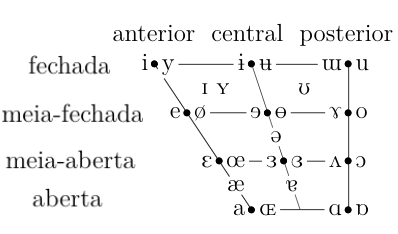
\includegraphics[width=0.45\linewidth]{img/vowels.png}
    \caption{Vogais IPA}
    \label{fig:vowels_ipa}
\end{figure}

A ideia do AFI é mapear e caracterizar todos os sons das línguas humanas. Desse modo, cada língua aproveita apenas um subconjunto do AFI. Os fones presentes no Português-Brasileiro estão circulados. Levando em conta apenas o subconjunto dos fones do PB, e também tendo em mente que os símbolos do alfabeto fonético precisam ser transformados em código ASCII para serem interpretados, faz sentido construir uma nova tabela adaptada para o problema em questão. O resultado desta adaptação pode ser visto nas Tabelas \ref{tab:new_rep} e \ref{tab:new_vocals}. Nessas novas tabelas, além da exclusão de alguns pontos e modos de articulação (motivada pela própria natureza do PB), apresenta-se também uma chave de transcrição alternativa que engloba apenas caracteres pertencentes ao código ASCII. Com relação à tabela das vogais (\ref{tab:new_vocals}), a dimensão de arredondamento foi dispensada pois não havia mais a necessidade dessa marcação.

\begin{center}
\scalebox{0.9}{
    \begin{tabular}{|l|cc|cc|cc|cc|cc|}
        \hline & 
            \multicolumn{2}{|c|}{\footnotesize{Bilabial}} &					% Bilabial
            \multicolumn{2}{|c|}{\footnotesize{Lab. dent.}} & 			% Labiodental
            \multicolumn{2}{|c|}{\footnotesize{Alveolar}} & 				% Alveolar
            \multicolumn{2}{|c|}{\footnotesize{P-alveo.}} & 		% Post-alveolar

            \multicolumn{2}{|c|}{\footnotesize{Velar}} & 					% Velar  \\				

        \hline Plosive &  							% Plosive
            p & b &	% Bilabial
            &&	% Labiodental
            t & d	% Alveolar
            & &% Post-alveolar
            & k & g 										         \\								

        \hline Nasal & 							% Nasal
            & m 	% Bilabial
            &  &  & % Labiodental
            & n 	% Alveolar
            & & % Post-alveolar
            & & N \\	% Velar
                     	

        \hline Tap/Flap &  						% Tap /Flap
            &													% Bilabial
            & &														% Labiodental
           && r &					% Alveolar
            &&                 % Post-alveolar

            \BlankCell        & &        	% Vela

        \hline Fricative & 						% Fricative
            &  &									% Bilabial
            f & v &													% Labiodental
            s & z &													% Alveolar
            x & j &									% Post-alveolar
            h  & \\										

        \hline Lat. appr. & 					% Lat. Approx
            \BlankCell        & \BlankCell        &		% Bilabial
            \BlankCell        & \BlankCell        &		% Labiodental

           & l &							% Alveolar
                                                      &&                  % Post-alveolar
  
             & L  	
             &% Velar
         
        \hline
    \end{tabular}
}%scalebox
\captionof{table}{Consoantes na nova representação}\label{tab:new_rep}
\end{center}

\begin{center}
\begin{table}[H]
\begin{center}
    \begin{tabular}{lll}
        \hline
         & Anterior & Posterior \\
         \hline
        Fechada & i & u \\
        \hline
        Meia-fechada & e & o \\
        \hline
        Meia-aberta & E & O \\
        \hline
        Aberta & a &  \\
        \hline
        Nasais & A (ã) &\\ & 3 ($\tilde{e}$) &\\ 
        \hline
    \end{tabular}
\end{center}
\caption{Vogais na nova representação}
\label{tab:new_vocals}
\end{table}
\end{center}


 A Tabela \ref{tab:chave} exibe a chave de transcrição proposta utilizando as tabelas  fonéticas criadas e a Tabela \ref{tab:transc} exibe alguns exemplos de transcrições possíveis.  

\begin{table}[]
\begin{center}
\begin{tabular}{lc}
\textbf{AFI} & \multicolumn{1}{l}{\textbf{Transcrição Proposta}} \\ \hline

\textbf{{[}p{]}} - \textbf{p}arar & p \\
\textbf{{[}b{]}} - \textbf{b}otar & b \\
\textbf{{[}t{]}} - \textbf{t}ocar & t \\
\textbf{{[}d{]}} - \textbf{d}ançar & d \\
\textbf{{[}k{]}} - \textbf{c}asar & k \\
\textbf{{[}g{]}} - \textbf{g}ostar & g \\
\textbf{{[}f{]}} - \textbf{f}ugir & f \\
\textbf{{[}v{]}} - \textbf{v}oltar & v \\
\textbf{{[}s{]}} - \textbf{s}oltar & s \\
\textbf{{[}z{]}} - pre\textbf{s}enciar & z \\
\textbf{{[}\ipa{S}{]}} - \textbf{ch}amar & x \\
\textbf{{[}\ipa{Z}{]}} - \textbf{j}antar & j \\
\textbf{{[}t\ipa{S}{]}} - sen\textbf{t}ir & t \\
\textbf{{[}d\ipa{Z}{]}} - \textbf{d}izer & d \\
\textbf{{[}h{]}} - e\textbf{rr}ar & h \\
\textbf{{[}\ipa{\:r}{]}} - enca\textbf{r}ar & r \\
\textbf{{[}l{]}} - pu\textbf{l}ar & l \\
\textbf{{[}\textipa{L}{]}} - espa\textbf{lh}ar & L \\
\textbf{{[}m{]}} - \textbf{m}orar & m \\
\textbf{{[}n{]} }- \textbf{n}adar & n \\
\textbf{{[}\ipa{N}{]}} - so\textbf{nh}ar & N\\
\textbf{{[}a{]}} - p\textbf{a}rar & a \\
\textbf{{[}e{]}} - l\textbf{e}r & e \\
\textbf{{[}\textepsilon{]}} - esp\textbf{e}ro & E \\
\textbf{{[}i{]}} - r\textbf{i}r & i \\
\textbf{{[}o{]}} - pr\textbf{o}por & o \\
\textbf{{[}\textopeno{]} }- col\textbf{o}co & O \\
\textbf{{[}u{]}} - c\textbf{u}rtir & u \\
\textbf{{[}\~e{]}} - \textbf{e}ntreter & 3 \\
\textbf{{[}ã{]}} - pl\textbf{a}ntar & A \\
\textbf{{[}\~o{]}} - comp\textbf{o}nho & o \\
\textbf{{[}\textupsilon{]}} - cas\textbf{o} & u \\
\textbf{{[}j{]}} - sa\textbf{i}o & i \\
\textbf{{[}w{]}} - vo\textbf{l}to & u
\end{tabular}
\end{center}
\caption{Chave de Transcrição Proposta}
\label{tab:chave}
\end{table}

\begin{table}[]
\begin{center}
\begin{tabular}{cc}
\hline
\textbf{Verbo} & \textbf{Transcrição} \\ \hline
ressentir & hes3ntir \\
paro & paru \\
possuo & posuu \\
olha & oLa \\
sacudir & sakudir \\
voltar & voutar \\ \hline
\end{tabular}
\end{center}
\caption{Exemplos de Transcrições}
\label{tab:transc}
\end{table}



\section{Corpus}
\label{sec:corpus}
O corpus utilizado para o treinamento dessa rede foi construído a partir da listagem de verbos contida no enderenço \texturl{www.conjugação.com.br}.

Primeiramente, foi realizada uma etapa de extração dos verbos e suas respectivas formas flexionadas para um arquivo \textit{.csv} via técnica de \textit{webscraping}, uma técnica que extrai informações contidas nas páginas da web (\cite{mitchell:2015}). Em seguida, os verbos irregulares foram selecionados manualmente para diferentes famílias de verbos, ou seja, grupos que continham o mesmo padrão de flexão. Alguns dos verbos irregulares listados na fonte de referência não eram irregulares no processo de flexão de interesse, e portanto foram realocados para o grupo de verbos regulares (vide exemplo do verbo \textit{correr} na Seção \ref{sec:escopo}). Na sequência, os verbos  coletados na forma infinitiva tiveram o fone /\textit{r}/ extraído para que no \textit{input} do modelo entrasse apenas o radical + vogal temática dos verbos.

 Um experimento foi realizado na tentativa de utilizar o transcritor fonético automático disponibilizado por \cite{guide:2016} para tornar o processo de transcrição mais rápido. Entretanto, o transcritor falhou na tentativa de transcrever verbos cujas escritas coincidem com substantivos, como por exemplo “apoio”, “peso”, “toco”, “posto”, “jogo”, entre outros. Desse modo, os verbos coletados foram transcritos manualmente utilizando a chave de transcrição apresentada na Tabela \ref{tab:chave}. No total, foram obtidos 423 verbos, 83 a menos que no experimento realizado por (\cite{rumelhart:1986}).

Dos 423 verbos extraídos, 20 foram considerados verbos sem possível agrupamento (verbos como “ir”, “trazer” e “saber”), totalizando uma base de 214 verbos regulares e 209 irregulares (50.6\% e 49.4\% respectivamente). A título de comparação, o estudo de Rumelhart \& McClelland (\citeyear{rumelhart:1986}) era composto por apenas 20\% de verbos irregulares.

A Tabela \ref{tab:classes} associa exemplos das classes obtidas à sua respectiva contagem e proporção no corpus.

\begin{table}[H]
\begin{center}
\begin{tabular}{|l|c|c|c|}
\toprule
 & Exemplos & Contagem & Proporção\\
\midrule
1  & ansia, anseio & 9 & 2.13\%\\
2  & bota, boto & 30 & 7.09\%\\
3  & cobri, cubro & 7 & 1.65\%\\
4  & dize, digo & 7 & 1.65\%\\
5 & faze, faço & 15 & 3.55\%\\
6  & cre, creio & 5 & 1.18\%\\
7  & senti, sinto & 8 & 1.89\% \\
8  & pedi, peço & 7 & 1.65\%\\
9  & pô, ponho & 27 & 6.38\%\\
10  & segui, sigo & 27 & 6.38\%\\
11  & te, tenho & 10 & 2.36\%\\
12  & testa, testo & 20 & 4.73\%\\
13  & ve, vejo & 6 & 1.42\%\\
14  & vi, venho & 10 & 2.60\%\\
15 & sabe, sei & 20 & 4.73\%\\
16  & fala, falo & 214 & 50.59\%\\
\bottomrule
\end{tabular}
\end{center}
\captionof{table}{Organização do corpus}
\label{tab:classes}
\end{table}

Apesar do volume de verbos irregulares ser consideravelmente maior do que o volume utilizado no estudo de \cite{rumelhart:1986}, pode-se dizer que algumas das famílias coletadas apresentam certa improdutividade, no sentido de que muitos verbos são reaproveitamentos de outros através do uso de prefixos. Por exemplo, a família do verbo “fazer” é composta apenas de verbos derivados do mesmo: “desfazer”, “refazer”, etc. Isto pode ser observado em outras classes, como a do verbo “cobrir”, “pedir”, “dizer”, “ver”, entre outras. As classes com maior variabilidade são as do verbo “botar” com por exemplo “tocar”, “gostar”, “colocar”; “testar” com “pegar”, “secar”, “testar”; e “seguir” com “digerir”, “regredir”, “divertir”.   

\subsection{Types x Tokens}
Outra questão importante a respeito do corpus utilizado, refere-se à frequência em que os verbos serão inseridos no modelo. Para isso, introduzimos os conceitos de \textit{word type} e \textit{word token} (\cite{Manning:1999}). Discutir sobre a frequência em que os verbos são inseridos é relevante, pois o treinamento das Redes Neurais se dá por meio de \textit{ciclos}. Como vimos no Cap. \ref{ch:01}, \cite{rumelhart:1986} conseguiram fabricar o comportamento da \textit{Curva de Desenvolvimento em U} ao manipular a frequência de inserção dos dados, privilegiando verbos irregulares. 

O termo \textit{type}, importado da área de \textit{Processamento de Linguagem Natural}, refere-se ao número de palavras \textbf{únicas} presentes em um Corpus. A frase “Essa frase é uma frase de exemplo.”, portanto, possui 6 \textit{types}. O termo \textit{token}, em contrapartida, refere-se ao número total de termos presentes, incluindo as repetições. Nesse caso, a mesma frase de exemplo possui 7 \textit{tokens}. 

Evidências na área de psicolinguística (\cite{Bybee:1995,janet:2018}) indicam que humanos aprendem a generalizar padrões fonológicos baseado na contagem de \textit{word types}, ignorando a frequência de uso das palavras. Com isso, nesta pesquisa cada verbo é visto como um \textit{word type}. Isso significa que a frequência de uso dos verbos não foi levada em consideração para a introdução dos mesmos no modelo. Ao invés disso, os verbos são tratados de forma igualitária e compartilham do mesmo número de inserções.\\


\subsection{Os Inputs do Modelo Encoder-Decoder}
\label{sec:inputs}

Após a construção do corpus, os verbos transcritos tiveram seus respectivos fones associados a um dicionário de traços fonéticos, os mesmos traços que originaram as Tabelas \ref{tab:new_rep} e \ref{tab:new_vocals}. A Tabela \ref{tab:pOsu} apresenta um exemplo desse processo para o verbo “posso” - “\textit{pOsu}”. 

\begin{table}[H]
\begin{center}
\begin{tabular}{lll}
Fone & Traços Fonéticos &  \\ \cline{1-2}
p & bilabial, oclusiva, surda &  \\
O & meio-aberta, posterior &  \\
s & fricativa, alveolar, surda &  \\
u & fechada, posterior & 
\end{tabular}
\end{center}
\caption{Traços Fonéticos para o Verbo “Posso“}
\label{tab:pOsu}
\end{table}

Na computação, um dicionário é uma estrutura de armazenamento de dados que associa uma chave a um valor. Essa estrutura possui um conjunto mutuamente exclusivo de chaves, cada uma associada a um valor. Desse modo, ao consultar um dicionário com um valor chave, a estrutura retorna como resposta o valor associado.

 No total são necessários 20 traços para representar um fone. São 18 para representar os traços das tabelas fonéticas construídas (\ref{tab:new_rep} e \ref{tab:new_rep}): Oclusivo, Nasal, Tepe, Fricativa, Aproximante Lateral, Bilabial, Labio-Dental, Alveolar, Pós-Alveolar, Velar, Glotal, Fechada, Meia-fechada, Meia-aberta, Aberta, Anterior, Posterior; e 2 para representar início e final do verbo ($<$beg$>$ e $<$end$>$).

Os fones são então caracterizados pela presença (1) e ausência (0) dos traços mencionados. Desse modo, o dicionário construído possui fones nos valores das chaves e uma lista de 0's e 1's para representar as presenças e ausências dos traços fonéticos. De acordo com as tabelas fonéticas desenvolvidas, cada fonema pode ser descrito por apenas três ou dois traços fonéticos, de modo que cada vetor terá apenas três ou dois valores marcados como \textbf{1}'s. Os \textit{tokens} de início e final do verbo ($<$beg$>$ e $<$end$>$) são exceções, com apenas uma marcação de presença no vetor. 

A Tabela \ref{tab:coding_example} mostra como exemplo uma comparação entre dois fones similares (\textbf{p} e \textbf{b}) que distinguem-se apenas pelo traço fonético sonoro. O resultado é uma representação vetorial que também carrega essa noção de proximidade entre os fones. O começo do verbo é representado por um vetor que marca 0 em todos os traços fonéticos e 1 no \textit{token} de começo (o traço de fim pode ser compreendido de maneira análoga). 

\begin{table}[H]
\begin{center}
\begin{tabular}{lll}
\textbf{ Traço} & \textbf{p} &\textbf{ b} \\
 \toprule
oclusiva & 1 & 1 \\
nasal & 0 & 0 \\
tepe & 0 & 0 \\
fricativa & 0 & 0 \\
l-aprox & 0 & 0 \\
bilabial & 1 & 1 \\
labiodental & 0 & 0 \\
alveolar & 0 & 0 \\
p-alveolar & 0 & 0 \\
velar & 0 & 0 \\
glotal & 0 & 0 \\
sonora & 0 & 1 \\
fechada & 0 & 0 \\
m-fechada & 0 & 0 \\
m-aberta & 0 & 0 \\
aberta & 0 & 0 \\
anterior & 0 & 0 \\
posterior & 0 & 0 \\
<beg> & 0 & 0 \\
<end> & 0 & 0
\end{tabular}
\end{center}
\caption{Exemplo de Codificação de fones}
\label{tab:coding_example}
\end{table}

Por fim, juntando todos os passos expostos, o processo completo de transformação dos inputs pode ser resumido a:

\begin{enumerate}
    \item Adição dos \textit{tokens} de início e final dos verbos.
    \item Divisão dos verbos em fones, seguindo chave de transcrição proposta.
    \item Transformação dos fones em \textit{arrays} de 0's e 1's, seguindo o dicionário de fones desenvolvido.
\end{enumerate}








\chapter{Introdução a Redes Neurais}
\label{ch:03}


% \epigraph{\itshape Those who cannot remember the past are condemned to compute it.''}{---Steven Pinker, \textit{Words and Rules}}

\section{Redes Neurais}

Uma rede neural é, essencialmente, um modelo de aprendizado de máquina supervisionado %[ref] 
que está a procura de aprender \textit{padrões}. Um modelo de aprendizado de máquina é uma tarefa computacional que explora algoritmos que podem aprender a partir de seus erros e fazer previsões sobre dados. A principal característica desse tipo de modelo é o caráter indutivo dos algoritmos, em oposição aos dedutivos. Esse tipo de algoritmo é normalmente inicializado com nenhuma expectativa sobre a tarefa que deve realizar e busca informações exclusivamente a partir dos dados do problema. Os possíveis tipos de aprendizado de máquina são divididos entre: \textit{supervisionados}, \textit{não-supervisionados} %ref
e por \textit{reforço}. %ref
No caso das redes neurais, o aprendizado diz-se supervisionado, pois informa-se à rede o \textit{output} esperado pelo treinamento.

A inspiração para o desenvolvimento da modelagem em redes neurais aritificiais surgiu a partir de estudos em neurosciência %[ref] 
que concluiram que, diante de múltiplas apresentações de um mesmo estímulo, um mesmo grupo de neurônios sofre incitação e dispara (\cite{hubel:1962}).  Analogamente, o modelo artificial é composto por uma camada de \textit{input} que recebe diferentes estímulos (vetores numéricos que representam o objeto a ser analisado). A informação recebida é distribuída ao longo de múltiplas conexões com a próxima camada através de uma múltiplicação com uma matriz de pesos $\vect{W}$. A matriz de pesos funciona como uma analogia às conexões existentes entre neurônios de modo que um peso maior representa uma conexão que deve ser reforçada e um peso menor representa uma conexão que deve ser reprimida. Além disso, é importante que o sistema de aprendizado não seja demasiado sensível a todo \textit{input} que receber, pois nesse caso cada \textit{input} diferente recebido alteraria completamente o modelo impossibilitando um aprendizado generalizado. Como solução, o resultado obtido a partir da multiplicação dos pesos pelos \textit{inputs} entra como argumento em uma função de ativação. A função de ativação é uma função que simula o potencial energético existente entre as conexões neurais e permite que uma unidade apenas seja ativada caso o resultado dessa função atinja um \textit{threshold} mínimo. Isso permite ao sistema a produção de diferentes respostas para padrões diferentes utilizando a mesma rede e além disso, permite que o aprendizado ocorra de forma gradual, de modo que o efeito de estímulos passados ainda perdure por um longo período mesmo após a apresentação de novos estímulos. Uma das funções de ativação mais utilizadas na literatura (e inclusive utilizada pelos pesquisadores Rumelhart e McClelland) é a função \textit{Sigmoid}, uma função suave, diferenciável e facilmente interpretável. A Fig. \ref{fig:sigmoidplot} ilustra o processo de ativação dado um \textit{input} $\vect{x}$. Supõe-se que um neurônio seja ativado apenas se houver uma energia mínima para tal. Da mesma forma, representa-se uma ativação no eixo \textit{y} (com valores entre 0 (não ativação) e 1 (ativação)) de modo que apenas valores mais altos de $\vect{x}$ atingem valores próximos da ativação em \textit{y}.

\begin{figure}[H]
\begin{tikzpicture}
    \begin{axis}[
    	legend pos=north west,
        axis x line=middle,
        axis y line=middle,
        x tick label style={/pgf/number format/fixed,
                            /pgf/number format/fixed zerofill,
                            /pgf/number format/precision=1},
        y tick label style={/pgf/number format/fixed,
                            /pgf/number format/fixed zerofill,
                            /pgf/number format/precision=1},
        grid = major,
        width=16cm,
        height=8cm,
        grid style={dashed, gray!30},
        xmin=-1,     % start the diagram at this x-coordinate
        xmax= 1,    % end   the diagram at this x-coordinate
        ymin= 0,     % start the diagram at this y-coordinate
        ymax= 1,   % end   the diagram at this y-coordinate
        %axis background/.style={fill=white},
        xlabel=x,
        ylabel=y,
        tick align=outside,
        enlargelimits=false]
      % plot the stirling-formulae
      \addplot[domain=-1:1, black, thick,samples=500] {1/(1+exp(-5*x))};
      %\addplot[domain=-1:1, blue, ultra thick,samples=500] {1/(1+exp(-10*x))};
      \addlegendentry{$f(x)=\frac{1}{1+e^{-ax}}$}
      %\addlegendentry{$g(x)=\frac{1}{1+e^{-10x}}$}
    \end{axis} 
\end{tikzpicture}
\caption{A função logística utilizada para o cálculo da probabilidade de ativação.}
\label{fig:sigmoidplot}
\end{figure} %diminuir esse desenho

Após essa passagem pela função de ativação, o resultado serve como novo input para a próxima camada e assim sucessivamente até a última, a camada de \textit{output}. Todas as camadas existentes entre as camadas de \textit{input} e de \textit{output} são chamadas de \textit{camadas escondidas} (Ver Fig. \ref{fig:ffd}.)

% \begin{align}\label{eq:sigmoid}
% p(w_{i} = 1) = \frac{1}{1+e^{\sum_{i} w_{i}x_{i}}}
% \end{align}

Algebricamente, pode-se representar o processo descrito através da composição de múltiplas funções, uma vez que o resultado das operações precedentes servirão como entrada para as próximas camadas.

\begin{align}
% f(\vect{x}) &= f^{(2)}(f^{(1)}(\vect{x}; \vect{W}_1); \vect{W}_2)\\
% &= 
\sigma(\vect{W}_2 (\sigma(\vect{W}_1\vect{x})))
\end{align}

\definecolor{blue}{RGB}{159, 192, 176}
\definecolor{green}{RGB}{160, 227, 127}
\definecolor{orange}{RGB}{243, 188, 125}
\definecolor{red}{RGB}{253, 123, 84}
\definecolor{nephritis}{RGB}{39, 174, 96}
\definecolor{emerald}{RGB}{46, 204, 113}
\definecolor{turquoise}{RGB}{39, 174, 96}
\definecolor{green-sea}{RGB}{22, 160, 133}
\definecolor{purple}{RGB}{181, 124, 215}
% Tikzstyles for Computation Graphs

% nodes
\tikzstyle{noop} = [circle, draw=none, fill=red, minimum size = 10pt]
\tikzstyle{op} = [circle, draw=red, line width=1.5pt, fill=red!70, text=black, text centered, font=\bf \normalsize, minimum size = 25pt]

\tikzstyle{opintense} = [circle, draw=red, line width=1.5pt, fill=red!150, text=black, text centered, font=\bf \normalsize, minimum size = 25pt]


%new style
\tikzstyle{gp} = [circle, draw=red, line width=4pt, text=black, text centered, font=\bf \normalsize, minimum size = 4.cm]

\tikzstyle{box} = [rectangle, draw=red, line width=1.5pt, fill=red!70, text=black, align=center, font=\bf \normalsize, minimum size = 45pt]

\tikzstyle{box2} = [rectangle, draw=black, line width=0.9pt, text=black, align=center, font=\bf \normalsize, minimum size = 20pt]

\tikzstyle{box3} = [rectangle, draw=black, line width=0.9pt, fill=black, text=black, align=center, font=\bf \normalsize, minimum size = 20pt]

\tikzstyle{state} = [circle, draw=blue, line width=1.5pt, fill=blue!70, text=black, text centered, font=\bf \normalsize, minimum size = 25pt]

\tikzstyle{output} = [circle, draw=purple, line width=1.5pt, fill=purple!70, text=black, text centered, font=\bf \normalsize, minimum size = 25pt]


\tikzstyle{gradient} = [circle, draw=nephritis, line width=1.5pt, fill=nephritis!60, text=black, text centered, font=\bf \normalsize, minimum size = 25pt]
\tikzstyle{textonly} = [draw=none, fill=none, text centered, font=\bf \normalsize]
\tikzstyle{boxtextonly} = [draw=none, fill=none, align=center, font=\bf \normalsize]

\tikzstyle{normal} = [circle, draw=black, line width=1.0pt, fill=none, text=black, text centered, font=\bf \normalsize, minimum size = 20pt]


% edges
\tikzstyle{tedge}  = [draw, thick, >=latex, ->]
\tikzstyle{tedge_dashed}  = [draw, thick, >=latex, ->, dashed]
\tikzstyle{nedge}  = [draw, thick, >=latex]
\tikzstyle{nedge_dashed}  = [draw, thick, >=latex, dashed]


% namedscope
\tikzstyle{namedscope} = [circle, draw=orange, line width=1.5pt, fill=orange!60, align=center, inner sep=0pt]
\begin{figure}[ht!]
\centering

\scalebox{1.0}{
\begin{tikzpicture}[auto]

% operations =========

% FNN input
\node[normal] (x1) {};
\node[textonly, above=10pt of x1] (input) {Camada de \textit{inputs}};
\node[normal, below=10pt of x1] (x2) {};
\node[normal, below=10pt of x2] (x3) {};
\node[normal, below=10pt of x3] (x4) {};
\node[normal, below=10pt of x4] (x5) {};
\node[normal, below=10pt of x5] (x6) {};

% FNN output
\node[textonly, right=50pt of x1] (center) {Camada Escondida};
\node[normal, below=25pt of center] (y1) {};
\node[normal, below=10pt of y1] (y2) {};
\node[normal, below=10pt of y2] (y3) {};

% FNN output
\node[textonly, right=110pt of input] (output) {Camada de \textit{outputs}};
\node[normal, below=15pt of output] (z1) {};

\node[normal, below=10pt of z1] (z2) {};
\node[normal, below=10pt of z2] (z3) {};
\node[normal, below=10pt of z3] (z4) {};
\node[normal, below=10pt of z4] (z5) {};
\node[normal, below=10pt of z5] (z6) {};

% phon features 2

% edges FNN
\path[nedge] (x1) -- (y1);
\path[nedge] (x1) -- (y2);
\path[nedge] (x1) -- (y3);

\path[nedge] (x2) -- (y1);
\path[nedge] (x2) -- (y2);
\path[nedge] (x2) -- (y3);

\path[nedge] (x3) -- (y1);
\path[nedge] (x3) -- (y2);
\path[nedge] (x3) -- (y3);

\path[nedge] (x4) -- (y1);
\path[nedge] (x4) -- (y2);
\path[nedge] (x4) -- (y3);

\path[nedge] (x5) -- (y1);
\path[nedge] (x5) -- (y2);
\path[nedge] (x5) -- (y3);

\path[nedge] (x6) -- (y1);
\path[nedge] (x6) -- (y2);
\path[nedge] (x6) -- (y3);

% edges FNN
\path[nedge] (y1) -- (z1);
\path[nedge] (y1) -- (z2);
\path[nedge] (y1) -- (z3);
\path[nedge] (y1) -- (z4);
\path[nedge] (y1) -- (z5);
\path[nedge] (y1) -- (z6);
\path[nedge] (y2) -- (z1);
\path[nedge] (y2) -- (z2);
\path[nedge] (y2) -- (z3);
\path[nedge] (y2) -- (z4);
\path[nedge] (y2) -- (z5);
\path[nedge] (y2) -- (z6);
\path[nedge] (y3) -- (z1);
\path[nedge] (y3) -- (z2);
\path[nedge] (y3) -- (z3);
\path[nedge] (y3) -- (z4);
\path[nedge] (y3) -- (z5);
\path[nedge] (y3) -- (z6);

\end{tikzpicture}
}\caption{Esquema de uma rede neural do tipo Feedforward} 
\label{fig:ffd}
\end{figure}

\subsection{Treinamento}

Para que a rede seja capaz de identificar os padrões desejados, é necessário alimentá-la com o que se espera como resposta (\textit{targets}), pois o treinamento da mesma consiste, essencialmente, na atualização das matrizes de pesos que deve ocorrer a partir da comparação entre os valores previstos pela rede (\textit{outputs}) e os \textit{targets}. A comparação entre esses valores se dá por meio de uma função de custo (\textit{Loss Function}), que representa uma forma de se quantificar o quão perto se está de uma rede ideal em que os resultados previstos correspondam exatamente aos \textit{targets}. O objetivo do aprendizado da rede é minimizar essa diferença, ou seja, encontrar o mínimo da função de custo (\cite{josh:2017}). Após a exposição a um certo número de exemplos, todos os pesos são atualizados simultaneamente com os valores que em conjunto minimizam a função de custo e portanto aproximam as previsões da rede aos \textit{targets}. %ref

\section{Modelo Apresentado por Rumelhart e McClelland (1986)}
\label{sec:arqFDD}

O esquema apresentado pelos pesquisadores Rumelhart e McClelland represetado na Fig. \ref{fig:esquemafdd} é conhecido como uma arquitetura do tipo \textit{Feedforward-Network (FFD)} sem camadas escondidas. Nesse caso, todos os nódulos da camada de input se conectam diretamente aos nódulos da camada de output.

Relembrar a representação explicada no cap 2, mostrar o input e output da rede deles, colocar alguns resultados que eles obtiveram.

% \subsection{Wickelfeatures}
% \label{sec:wickelfeatures}
% %repensar nessa seçao após o desenvolvimento do texto de traços fonológicos
% Os pesquisadores Rumelhart e McClelland propõem a caracterização de cada fonema como uma combinação simplificada de traços distintivos em apenas 4 dimensões. O fone \textit{d}, por exemplo, é caracterizado por um conjunto de 4 traços: "Int.", indicando que é uma consoante interrompida; "V", indicando a vibração das cordas vocais; "Oclusi."  indicando que é uma consoante oclusiva; e foi caracterizado como um fone de ponto de articulação "Médio" já que o fone \textit{b}, além de compartilhar das mesmas dimensões, apresenta ponto de articulação anterior ao \textit{d}. Seguindo este raciocínio para uma representação simplificada dos fonemas, os pesquisadores apresentam uma tabela que codifica cada fonema na língua inglesa às quatro dimensões de traços. A Tabela \ref{tab:Tab1} foi baseada nesse sistema de codificação, porém com algumas adaptações para o português brasileiro. A tabela original apresentada pelos autores pode ser consultada no Apêndice \ref{ch07-appendice}. A primeira dimensão da tabela divide os fonemas em três grandes grupos: consoantes interrompidas, continuadas ou vogais. Dentre as consoantes interrompidas, encontram-se as consoantes oclusivas e nasais. Vê-se que nem todos os fonemas da tabela internacional (\ref{tab:ipa1} e \ref{tab:ipa2}) foram mapeados, apenas os mais importantes para a língua. Com relação às consoantes continuadas, estas foram subdivididas entre fricativas e líquidas (a versão dos autores ainda agrupava semi-vogais às líquidas). Ainda nesta dimensão, as vogais foram simplificadas a apenas altas ou baixas.  Com relação ao ponto de articulação (terceira dimensão), os autores agruparam bilabiais e labio-dentais em um único atributo entitulado de "anterior". Dentais e alveolares são consideradas consoantes com ponto de articulação médio. Pós-alveolares em diante são consideradas posteriores. A quarta dimensão subcategoriza as consoantes em vozeadas (V) vs. não-vozeadas (U) e as vogais em longas (L) e curtas (S). No caso da língua portuguesa não ocorre essa distinção entre as vogais, portanto essa dimensão é utilizada apenas para a dinstinção das vogais entre abertas e fechadas. No caso da vogal "u", na versão original apresentada pelos pesquisadores, ela representava a vogal curta associada à palavra \textit{book} (/buk/) e foi mantida nessa mesma posição.

% A presença de cada um destes traços em cada dimensão para um determinado fonema recebe o valor $1$, enquanto que a ausência, $0$. A primeira dimensão diz respeito à ordem Int - Cont - Vogal e um fonema é associado a um único atributo desta dimensão, ou seja, se o fonema for uma consoante interrompida, ele deve ser representado pelo vetor (100), se o fonema for uma consoante continuada, deve ser representado pelo vetor (010) e se for vogal, pelo vetor (001). O mesmo serve para as demais dimensões, sendo que a ordem da segunda é: Ocl - Nasal (dado que a primeira dimensão é uma consoante interrompida); Fricat - Liq (dado que a primeira dimensão é uma consoante continuada) ou Alta - Baixa caso a primeira dimensão aponte para uma vogal. Em seguida a terceira dimensão diz respeito à ordem: Anterior - Médio - Posterior. Por último, a interpretação da quarta dimensão também está condicionada à primeira dimensão, ou seja, caso o fonema seja uma consoante ele pode ser vozeado ou não-vozeado; caso seja uma vogal, longa ou curta. 
% Com base na Tabela \ref{tab:Tab1}, portanto, o fonema \textit{d} passa a ser representado pelo vetor \ref{fond}. Cada sequência contida entre parênteses representa uma dimensão e os números dentro dela representam o atributo deste fonema nesta respectiva dimensão.

% \begin{align}
% d \Rightarrow (100)(10)(010)(10)\label{fond}
% \end{align}

% Com essa tabela, o sistema de codificação para um único fonema está completo, porém é imprescindível que a própria sequência fonológica também seja representada já que cada fonema constitui parte de uma sequência e os padrões devem ser encontrados levando-se em consideração essa sequência. Desse modo, os pesquisadores optam por representar, em cada vetor de \textit{input}, uma sequência de três traços (um trigrama de traços) para cada uma das dimensões propostas (vogal - vogal - int, por exemplo). Além disso, foi acrescentada uma última dimensão para representar início ou final de palavra, representado pelo símbolo "\#". Desse modo, \ref{token1}, \ref{token2} e \ref{token3} exibem as representações vetoriais do símbolo de fronteira e dos fonemas \textit{d} e \textit{a} considerando a última dimensão mencionada.

% \begin{align}
% \# \Rightarrow (000)(00)(000)(00)(1)\label{token1}\\
% d \Rightarrow (100)(10)(010)(10)(0)\label{token2}\\
% a \Rightarrow (001)(01)(010)(01)(0)\label{token3}
% \end{align}

% Por fim, define-se como um \textit{Wickelfeature} cada sequência de três traços fonológicos. Para alimentar a rede, os autores mapeiam cada verbo a um vetor booleano de tamanho 460, em que cada um destes valores representa a presença (ou ausência) de um \textit{Wickelfeature}. Em resumo, a rede completa é composta por duas camadas paralelas (\textit{input} e \textit{output} com 460 unidades de Wickelfeatures cada uma (Ver Fig. \ref{fig:esquemafdd}). 


% \begin{table}[ht!]
% \center
%     \begin{tabular}{lrrrrrrr}\toprule
%         &\multicolumn{2}{c}
% {}&\multicolumn{1}{c}     {\textbf{Anterior}}&\multicolumn{2}{c}{\textbf{Médio}}&\multicolumn{2}{c}{\textbf{Posterior}}
%         \\\cmidrule(r){3-4}\cmidrule(r){5-6}\cmidrule(r){7-8}   
%         &&V/L&U/S&V/L&U/S&V/L&U/S\\\midrule
%         Int.&   Oclusi. & b & p
%                 & d & t
%                 & g & k\\
%                 &Nasal & m
%                 & & n
%                 & & 
%                 & \\
%         Cont. & Fricat. & v& f
%                 & z & s
%                 & j & S\\
%                 &Liq. &l
%                 & &r
%                 & &
%                 & h*\\
%         Vogal & Alta & e & i 
%                 &   &  
%                 & o & u*\\
%               & Baixa & a & E
%               & &
%               & & O
%         \\\bottomrule
%         Codificação: S = \ipa{S};&  j = \ipa{Z};& h\footnote{h* = Apesar de representar uma fricativa posterior, foi mantido nesta posição assim como na tabela proposta em \ref{fig:table-eng}} = x;& E = \textepsilon; & O = \textopeno & u\footnote{u* = u \& \textupsilon} & &
%     \end{tabular}
%     \caption{Categorização de fonemas em quatro dimensões adaptada ao Português Brasileiro}\label{tab:Tab1}
% \end{table} 


% \begin{center}
% \scalebox{0.9}{
%     \begin{tabular}{|l|cc|cc|cc|cc|cc|cc|cc|cc|cc|cc|cc|}
% %\begin{tabular}{|l|cc|}
%         \hline & 
%             \multicolumn{2}{|c|}{\footnotesize{Bilabial}} &					% Bilabial
%             \multicolumn{2}{|c|}{\footnotesize{Lab. dent.}} & 			% Labiodental
%             \multicolumn{2}{|c|}{\footnotesize{Dental}} & 					% Dental
%             \multicolumn{2}{|c|}{\footnotesize{Alveolar}} & 				% Alveolar
%             \multicolumn{2}{|c|}{\footnotesize{P-alveo.}} & 		% Post-alveolar
%             \multicolumn{2}{|c|}{\footnotesize{Retroflex}} & 				% Retroflex
%             \multicolumn{2}{|c|}{\footnotesize{Palatal}} & 					% Palatal
%             \multicolumn{2}{|c|}{\footnotesize{Velar}} & 					% Velar
%             \multicolumn{2}{|c|}{\footnotesize{Uvular}} & 					% Uvular
%             \multicolumn{2}{|c|}{\footnotesize{Pharyng.}} & 			% Pharyngeal
%             \multicolumn{2}{|c|}{\footnotesize{Glottal}}  \\					% Glottal

%         \hline Plosive &  							% Plosive
%             p & b &													% Bilabial
%             &&														% Labiodental
%             \multicolumn{3}{|r}{t}&							% Dental
%             \multicolumn{3}{l|}{d}&							% Alveolar
%                                                                         % Post-alveolar
%             \ipa{\:t} & \ipa{\:d}&									% Retroflex
%             c & \textbardotlessj &														% Palatal
%             k & g &													% Velar
%             q & \ipa{\;G} &										% Uvular
%             & \BlankCell        &								% Pharyngeal
%             \ipa{P}& \BlankCell         \\								% Glottal

%         \hline Nasal & 							% Nasal
%             & m &													% Bilabial
%             & \ipa{M} &											% Labiodental
%             \multicolumn{3}{|r}{}&								% Dental
%             \multicolumn{3}{l|}{n}&							% Alveolar
%                                                                         % Post-alveolar
%             & \ipa{\:n} &														% Retroflex
%             & \textltailn &														% Palatal
%             & \ipa{N} &														% Velar
%             & \ipa{\;N} &														% Uvular
%             \BlankCell        & \BlankCell        &		% Pharyngeal
%             \BlankCell        & \BlankCell         \\		% Glottal

%         \hline Trill &  								% Trill
%             & \ipa{\;B}&											% Bilabial
%             & &														% Labiodental
%             \multicolumn{3}{|r}{}&								% Dental
%             \multicolumn{3}{l|}{r}&								% Alveolar
%                                                                         % Post-alveolar
%             & &														% Retroflex
%             & &														% Palatal
%             \BlankCell        & \BlankCell        &		% Velar
%             & \ipa{\;R}&											% Uvular
%             & &														% Pharyngeal
%             \BlankCell        & \BlankCell         \\		% Glottal

%         \hline Tap/Flap &  						% Tap /Flap
%             & &													% Bilabial
%             & &														% Labiodental
%             \multicolumn{3}{|r}{} &					% Dental
%             \multicolumn{3}{l|}{\ipa{R}} &					% Alveolar
%                                                                         % Post-alveolar
%             & \ipa{\:r} &														% Retroflex
%             & &														% Palatal
%             \BlankCell        & \BlankCell        &		% Velar
%             & &														% Uvular
%             & &														% Pharyngeal
%             \BlankCell        & \BlankCell         \\		% Glottal

%         \hline Fricative & 						% Fricative
%             \ipa{F} & \ipa{B} &									% Bilabial
%             f & v &													% Labiodental
%             \ipa{T} & \ipa{D} &									% Dental
%             s & z &													% Alveolar
%             \ipa{S} & \ipa{Z} &									% Post-alveolar
%             \ipa{\:s} & \ipa{\:z} &								% Retroflex
%             \ipa{\c{c}} & \ipa{J} &								% Palatal
%             x & \ipa{G} &											% Velar
%             \ipa{X} & \ipa{K} &									% Uvular
%             \textcrh & \ipa{Q} &								% Pharyngeal
%             h & \texthth \\										% Glottal

%         \hline Lat. Fric. & 					% Lat. Fricative
%             \BlankCell        & \BlankCell        &		% Bilabial
%             \BlankCell        & \BlankCell        &		% Labiodental
%             \multicolumn{3}{|r}{\textbeltl} &				% Dental
%             \multicolumn{3}{l|}{\textlyoghlig} &			% Alveolar
%                                                                         % Post-alveolar
%             & &														% Retroflex
%             & &														% Palatal
%             & &														% Velar
%             & &														% Uvular
%             \BlankCell        & \BlankCell        			% Pharyngeal
%             & \BlankCell        & \BlankCell         \\   % Glottal

%         \hline Approx & 							% Approx.
%             & &														% Bilabial
%             & \ipa{V} &											% Labiodental
%             \multicolumn{3}{|r}{}&								% Dental
%             \multicolumn{3}{l|}{\ipa{\*r}} &					% Alveolar
%                                                                         % Post-alveolar
%             & \ipa{\:R} &											% Retroflex
%             & j &														% Palatal
%             & \textturnmrleg &									% Velar
%             & &														% Uvular
%             & &														% Pharyngeal
%             \BlankCell        & \BlankCell         \\		% Glottal

%         \hline Lat. appr. & 					% Lat. Approx
%             \BlankCell        & \BlankCell        &		% Bilabial
%             \BlankCell        & \BlankCell        &		% Labiodental
%             \multicolumn{3}{|r}{}&								% Dental
%             \multicolumn{3}{l|}{l}&								% Alveolar
%                                                                         % Post-alveolar
%             & \ipa{\:l} &											% Retroflex
%             & \ipa{L} &												% Palatal
%             & \ipa{\;L} &											% Velar
%             & &														% Uvular
%             \BlankCell        & \BlankCell        &		% Pharyngeal
%             \BlankCell        & \BlankCell         \\		% Glottal
%         \hline
%     \end{tabular}
% }%scalebox
% \captionof{table}{Consoantes IPA}\label{tab:ipa1}
% \end{center}

% \begin{center}
%     \begin{vowel}
%         %    \putcvowel[l]{i}{1}
%         \putvowel[l]{i}{0pt}{0pt}
%         \putcvowel[r]{y}{1}
%         \putcvowel[l]{e}{2}
%         \putcvowel[r]{\o}{2}
%         \putcvowel[l]{\textepsilon}{3}
%         \putcvowel[r]{\oe}{3}
%         \putcvowel[l]{a}{4}
%         \putcvowel[r]{\textscoelig}{4}
%         \putcvowel[l]{\textscripta}{5}
%         \putcvowel[r]{\textturnscripta}{5}
%         \putcvowel[l]{\textturnv}{6}
%         \putcvowel[r]{\textopeno}{6}
%         \putcvowel[l]{\textramshorns}{7}
%         \putcvowel[r]{o}{7}
%         \putcvowel[l]{\textturnm}{8}
%         \putcvowel[r]{u}{8}
%         \putcvowel[l]{\textbari}{9}
%         \putcvowel[r]{\textbaru}{9}
%         \putcvowel[l]{\textreve}{10}
%         \putcvowel[r]{\textbaro}{10}
%         \putcvowel{\textschwa}{11}
%         \putcvowel[l]{\textrevepsilon}{12}
%         \putcvowel[r]{\textcloserevepsilon}{12}
%         \putcvowel{\textsci\ \textscy}{13}
%         \putcvowel{\textupsilon}{14}
%         \putcvowel{\textturna}{15}
%         \putcvowel{\ae}{16}
%     \end{vowel}
% \captionof{table}{Vogais IPA}\label{tab:ipa2}   
% \end{center} 


% \subsection{Codificação}


% \label{sec:cod}
% Cada verbo que participa da etapa de treinamento da rede passa por um processo inicial de codificação. Tal processo é descrito a seguir utilizando o verbo \textit{falar} como exemplo.\\ 

% \textbf{Entrada:} \textit{falar}\\

% \textbf{Passo 1:} O token de início e final de palavra é acrescentado e o grafema 'r' retirado:\\
% \hspace*{6.0em}      \#fala\#\\

% \textbf{Passo 2:} O verbo é segmentado em trigramas:\\
% \hspace*{6.0em}\#,f,a - f,a,l - a,l,a - la\#\\

% \textbf{Passo 3:} Cada trigrama tem seus fones associados aos seus respectivos traços fonológicos.

% No caso do trigrama "\#fa", por exemplo:
% \begin{itemize}
% \item \#,cont,vogal
% \item \#,cont,aberta
% \item \#,cont,anterior
% \item \#,cont,baixa

% \item \#,anterior,vogal
% \item \#,anterior,aberta
% \item \#,anterior,anterior
% \item \#,anterior,baixa

% \item \#,fric,vogal
% \item \#,fric,aberta
% \item \#,fric,anterior
% \item \#,fric,baixa

% \item \#,n-v,vogal
% \item \#,n-v,aberta
% \item \#,fn-v,anterior
% \item \#,n-v,baixa
% \end{itemize}


% \textbf{Passo 4:} Um dicionário associa cada fonema a um vetor de traços fonéticos, ou seja, toda possível combinação de traços foi mapeada e associada a um índice de um dicionário. \\

% \textbf{Passo 5:} Um dicionário de dimensão correspondente ao número total de \textit{Wickelfeatures} (460) é inicializado com $0's$ em todas as casas.\\

% \textbf{Passo 6:} Cada \textit{Wickelfeature} presente no verbo analisado altera o valor do dicionário para $1$.\\

% \textbf{Passo 7:} O dicionário resultante dos passos anteriores é utilizado como \textit{input} para a rede.

% \definecolor{blue}{RGB}{159, 192, 176}
\definecolor{green}{RGB}{160, 227, 127}
\definecolor{orange}{RGB}{243, 188, 125}
\definecolor{red}{RGB}{253, 123, 84}
\definecolor{nephritis}{RGB}{39, 174, 96}
\definecolor{emerald}{RGB}{46, 204, 113}
\definecolor{turquoise}{RGB}{39, 174, 96}
\definecolor{green-sea}{RGB}{22, 160, 133}
\definecolor{purple}{RGB}{181, 124, 215}
% Tikzstyles for Computation Graphs

% nodes
\tikzstyle{noop} = [circle, draw=none, fill=red, minimum size = 10pt]
\tikzstyle{op} = [circle, draw=red, line width=1.5pt, fill=red!70, text=black, text centered, font=\bf \normalsize, minimum size = 25pt]

\tikzstyle{opintense} = [circle, draw=red, line width=1.5pt, fill=red!150, text=black, text centered, font=\bf \normalsize, minimum size = 25pt]


%new style
\tikzstyle{gp} = [circle, draw=red, line width=4pt, text=black, text centered, font=\bf \normalsize, minimum size = 4.cm]

\tikzstyle{box} = [rectangle, draw=red, line width=1.5pt, fill=red!70, text=black, align=center, font=\bf \normalsize, minimum size = 45pt]

\tikzstyle{box2} = [rectangle, draw=black, line width=0.9pt, text=black, align=center, font=\bf \normalsize, minimum size = 20pt]

\tikzstyle{box3} = [rectangle, draw=black, line width=0.9pt, fill=black, text=black, align=center, font=\bf \normalsize, minimum size = 20pt]

\tikzstyle{state} = [circle, draw=blue, line width=1.5pt, fill=blue!70, text=black, text centered, font=\bf \normalsize, minimum size = 25pt]

\tikzstyle{output} = [circle, draw=purple, line width=1.5pt, fill=purple!70, text=black, text centered, font=\bf \normalsize, minimum size = 25pt]


\tikzstyle{gradient} = [circle, draw=nephritis, line width=1.5pt, fill=nephritis!60, text=black, text centered, font=\bf \normalsize, minimum size = 25pt]
\tikzstyle{textonly} = [draw=none, fill=none, text centered, font=\bf \normalsize]
\tikzstyle{boxtextonly} = [draw=none, fill=none, align=center, font=\bf \normalsize]

\tikzstyle{normal} = [circle, draw=black, line width=1.0pt, fill=none, text=black, text centered, font=\bf \normalsize, minimum size = 20pt]


% edges
\tikzstyle{tedge}  = [draw, thick, >=latex, ->]
\tikzstyle{tedge_dashed}  = [draw, thick, >=latex, ->, dashed]
\tikzstyle{nedge}  = [draw, thick, >=latex]
\tikzstyle{nedge_dashed}  = [draw, thick, >=latex, dashed]


% namedscope
\tikzstyle{namedscope} = [circle, draw=orange, line width=1.5pt, fill=orange!60, align=center, inner sep=0pt]
\begin{figure}[ht!]
\centering

\scalebox{1.0}{
\begin{tikzpicture}[H]

%vetor
\node[box2] (box1) {};
\node[box2, below=0pt of box1] (box2) {};
\node[box3, below=0pt of box2] (box3) {};
\node[box3, below=0pt of box3] (box4) {};
\node[textonly, below=0pt of box4] (box5) {\reflectbox{$\vdots$}};
\node[box3, below=0pt of box5] (box6) {};
\node[box3, below=0pt of box6] (box7) {};
\node[box2, below=0pt of box7] (box8) {};
\node[box3, below=0pt of box8] (box9) {};
\node[box2, below=0pt of box9] (box10) {};
\node[textonly, below=0pt of box10] (dim) {460x1};
\node[textonly, below=0pt of dim] (space) {};
%wickelfeatures
\node[textonly, right=20pt of box1] (wi1) {\#, oclusiva, média};
\node[textonly, right=20pt of box2] (wi2) {\#, anterior, fricativa};
\node[textonly, right=20pt of box3] (wi3) {\#, fricativa, vogal};
\node[textonly, right=20pt of box4] (wi4) {\#, contínua, anterior};
\node[textonly, right=20pt of box5] (wi5) {\reflectbox{$\vdots$}};
\node[textonly, right=20pt of box6] (wi6) {\#, não vozeada, aberta};
\node[textonly, right=20pt of box7] (wi7) {\#, contínua, posterior};
\node[textonly, right=20pt of box8] (wi8) {contínua, vogal, vogal };
\node[textonly, right=20pt of box9] (wi9) {contínua, vogal, líquida};
\node[textonly, right=20pt of box10] (wi10) {fricativa, posterior, \#};

%pré processamento
\node[textonly, left=230pt of box4] (verb1) {falar};
\node[textonly, below=10pt of verb1] (verb2) {fala};
\node[textonly, below=10pt of verb2] (verb3) {\#fala\#};

%trigramas
\node[textonly, right=20pt of verb1] (tri1) {\#,f,a};
\node[textonly, below=10pt of tri1] (tri2) {f,a,l};
\node[textonly, below=10pt of tri2] (tri3) {a,l,a};
\node[textonly, below=10pt of tri3] (tri4) {l,a,\#};

%features
\node[textonly, left=50pt of box2] (f1) {\#,cont,vogal};
\node[textonly, below=0pt of f1] (f2) {\#,cont,aberta};
\node[textonly, below=0pt of f2] (f3) {\#,cont,anterior};
\node[textonly, below=0pt of f3] (f4) {\#,cont,baixa};
\node[textonly, below=0pt of f4] (f5) {\reflectbox{$\vdots$}};
\end{tikzpicture}
}\caption{Esquema de Codificação de Wickelfeatures} 
\label{fig:wick}
\end{figure}

% \subsection{Decodificação}
% \label{sec:dec}

% Após o treinamento, a matriz de pesos foi atualizada e está pronta para realizar previsões. No entanto, é necessária a construção de uma função de decodificação, uma vez que a ativação dos \textit{outputs} representa a ativação de \textit{Wickelfeatures} e não de fonemas e tampouco verbos.

% A primeira parte da decodificação da rede envolve a seleção das unidades de Wickelfeatures que compõe o início da palavra reconstituída. Primeiramente, selecionam-se todas as unidades que tem como primeiro atributo o indicador de fronteira '\#'. Em seguida, dentre estas, observam-se os Wickelfeatures com maior score (mais próximos de terem sido ativados). Feita esta seleção, os fonemas \textit{competem} pelas features, ou seja, todos os fonemas que compartilham de uma mesma feature observada somam pontos. Ao final deste processo, espera-se que o fonema com mais pontos seja o fonema alvo da decodificação. Decodificam-se portanto os primeiros dois fonemas.

% A segunda parte do processo assemelha-se à primeira, porém ao invés da busca pelo trigrama inicial, selecionam-se todas as unidades que apresentam o atributo de fronteira na última posição. Em seguida ocorre o mesmo processo de competição para a decodificação dos dois últimos fonemas.

% A terceira parte do processo de decodificação envolve uma busca de compatibilidade entre os traços para os trigramas que não consitutem início ou final de palavra. Uma vez que o primeiro trigrama de fonemas foi decodificado, selecionam-se as próximas unidades cujas duas primeiras posições sejam compatíveis com as duas últimas do último trigrama decodificado. O processo de competição de fonemas se repete em um loop até que haja compatibilidade com o trigrama final, encontrado na segunda etapa.

% O maior problema desta função de decodificação encontra-se na etapa da busca pelos trigramas que não constituem início ou fim de palavra. Dependendo da sequência, é possível que dois ou mais trigramas compartilhem de muitas unidades de Wickelfeatures, ou seja, se um Wickelfeature for ativado, não há como representar sua ativação uma segunda ou terceira vez, a sua ativação acontece apenas uma vez. Isto pode interferir na etapa de seleção de compatibilidades, fazendo com que a função não consiga sair do loop pois continua selecionando os mesmos Wickelfeatures. Esse problema já foi apontado por \cite{Pinker:1999}.
% No livro, Pinker comenta a dificuldade da rede de Rumelhart e McClelland ao tentar decodificar a palavra 'algalgal' (uma palavra da língua Oykangand). Pinker faz uso desse exemplo pois, nesse caso, há inclusive a recorrência a nível de trigramas, mas o fato que é que mesmo a repetição a nível de \textit{Wickelfeatures} pode prejudicar a decodificação dos verbos. A probabilidade disso acontecer é ainda maior dependendo do comprimento dos verbos, e como apontado no Cap. \ref{ch:01-introduction}, os verbos da língua portuguesa possuem em média dois fonemas a mais que os verbos da língua inglesa. Como solução, foi necessária a implementação de uma função que considerasse apenas os trigramas fronteiriços. Desse modo foi possível verificar a capacidade da rede em capturar os processos de flexão irregulares que normalmente ocorrem no início ou no final das palavras. Para a palavra "postar", por exemplo, a irregularidade ocorre ao transmutar a vogal arredondada posterior semi-fechada para semi-aberta. Como essa irregularidade já pode ser detectada na primeira etapa da decodificação, pode-se avaliar o desempenho da rede baseado nesta etapa e desconsiderar a decodificação dos trigramas intermediários 'Ost' e 'stu' sem perda de informação.  

% Para concluir, a implementação de uma rede FFD para a predição de irregularidades verbais do português brasileiro mostrou-se uma tarefa de grande dificuldade e motivou a construção de novos tipos de arquitetura para o alcance dos objetivos propostos.



% A Qualificação foi até o ultimo paragrafo
%%%%%%%%%%%%%%%%%%%%%%%%%%%%%%%%%%%%%%%%%%%%%%%%%
%encerrar esse capitulo aqui

%Alguma Conclusão ou comentario sei la
% Uma vez que a arquitetura FFD gerou uma situação problemática, devido à própria natureza dos verbos em Português brasileiro somada às dificuldades encontradas no sistema de decodificação dos \textit{Wickelfeatures}, novas alternativas tiveram de ser investigadas. O problema, essencialmente, é relacionar sequências que influenciam umas às outras. Por exemplo, os verbos no infinitivo respeitam determinada lógica: são compostos por um radical mais um conjunto específico de terminações (\textit{ar, er, ir} e \textit{or}), e quando tal verbo é flexionado, é mandatório que determinadas regras relativas ao modo, tempo verbal e pessoa sejam respeitadas. Supondo que o verbo no infinitivo \textit{falar} seja conjugado na primeira pessoa do presente do indicativo, ou seja, \textit{falo}, neste caso, nota-se que o radical foi preservado e que a terminação foi alterada. Como esse processo de flexão verbal não é arbitrário e é possível inferir uma forma da outra, pode-se dizer que há um grau de subordinação entre os conjuntos de fonemas que compõe a forma infinitiva e a forma flexionada de cada verbo. Devido a uma condição fundamentalmente similar, uma analogia entre conjugação verbal e tradução de um idioma para outro pode ser estabelecida: ambos os processos obedecem a regras complexas consistentemente afim de preservar determinada coerência; na tradução a coerência semântica e sintática e na flexão verbal a lógica relativa a modo, tempo e pessoa. Visto que o problema é essencialmente o mesmo - processamento de sequências subordinadas - é de se supor que uma mesma técnica solucione ambas as situações, eis a implementação da função encoder-decoder, procedimento experimental utilizado, de acordo com a literatura mais atual (\cite{Goodfellow-et-al-2016}), em sistemas de tradução. Todavia, para a compreensão do funcionamento deste sistema, noções sobre Redes Neurais Recorrentes são indispensáveis, uma vez que a função encoder-decoder não passa de um mecanismo formado por tais redes.








\chapter{Encoder-Decoder}
\label{ch:05}


\section{Introdução ao Modelo Enconder-Decoder}
\label{sec:intro-sec-sec}
Um modelo de mapeamento \textit{Encoder-Decoder} (\cite{enc-dec:2014}) é um sistema composto por duas Redes Neurais Recorrentes cuja principal função é mapear uma relação entre duas sequências distintas que possuem uma relação paradigmática. Modelos do tipo \textit{Encoder-Decoder} (também conhecidos como \textit{Seq2Seq} (\cite{seq2seq:2014}) têm sido bastante utilizados em tarefas linguísticas, especialmente no desenvolvimento de sistemas de diálogo e em tradução automática.

Em um contexto de tradução, por exemplo, o modelo recebe como \textit{input }uma sequência de uma língua de origem e produz como \textit{output} uma sequência em uma língua alvo. A sequência gerada precisa, além de preservar o conteúdo semântico da sequência de origem, apresentar uma sintaxe aceita pelos falantes da língua alvo. 

\begin{figure}[ht!]
\centering
\begin{tikzpicture}
\node[punkt] (seq1) {Sequência 1};
\node[punkt, right=40pt of seq1] (seq2) {Sequência 2};

\path[tedge] (seq1) -- (seq2);

\node[punkt, below=40pt of seq2] (seq21) {O menino pequeno gosta do seu cachorro.};

\node[punkt, left=40 pt of seq21] (seq12) {The small boy likes his dog.};

\path[tedge] (seq12) -- (seq21);

\node[text, below=10 pt of seq21] (nada) {};

\end{tikzpicture}
\caption{Objetivo do Modelo Encoder-Decoder: Mapeamento de uma Sequência à Outra} 
\label{fig:seq2seq_simple}
\end{figure}
Observa-se no caso da tradução, que não há uma correspondência exata entre os termos de cada uma das línguas. A sentença na língua inglesa possui um termo a menos, sendo que o pronome “his” corresponde aos termos “do seu” no português. Além disso, observa-se que cada uma das línguas possui uma sintaxe diferente. No primeiro caso, o adjetivo \textit{small} se posiciona antes do substantivo \textit{boy}. No segundo, essa ordem é invertida (\textit{menino pequeno}). 

As duas redes recorrentes funcionam da seguinte maneira (ver Fig. \ref{fig:seq2seq}): uma primeira rede, a denominada \textit{Encoder} é alimentada com uma sentença da língua de origem (em inglês, por exemplo). Os termos dessa sentença entram um após o outro na rede e alimentam os \textit{estados} ($\vect{h}^{(t)}$), porém nesse caso não é necessário relacionar cada termo a um correspondente ($y_t$) como no caso do modelo de linguagem. A rede \textit{Encoder}, portanto, não possui \textit{alvos}, ela serve apenas para acumular os dados da língua de origem. Para tanto, o resultado do último estado, gerado após a inserção de todos os termos da sequência de origem, serve como estado inicial ($\vect{h}^{(0)}$) para uma segunda rede recorrente, denominada de \textit{Decoder}. A rede \textit{Decoder}, por sua vez, recebe como seu primeiro \textit{input}, um \textit{token} que representa o início da sequência alvo (\textbf{<beg>}), inicializando o modelo de linguagem dessa língua, como no modelo de rede neural recorrente apresentado na Seção \ref{sec:RNN}. 

 \begin{figure}[ht!]
\centering

\scalebox{0.9}{
\begin{tikzpicture}[
  hid/.style 2 args={
    rectangle split,
    rectangle split horizontal,
    draw=#2,
    rectangle split parts=#1,
    fill=#2!20,
    outer sep=1mm}]
  % draw input nodes
  \foreach \i [count=\step from 1] in {the,small,boy,{{$<$beg$>$}}}
    \node (i\step) at (2*\step, -2) {\i};

%write states    
\node[text, left = 2pt of i#1] (ht) {$\vect{h}^{(t)}$};

  % draw output nodes
  \foreach \t [count=\step from 4] in {o,menino,pequeno,{{$<$eos$>$}}} {
    \node[align=center] (o\step) at (2*\step, +2.75) {\t};
  }
  % draw embedding and hidden layers for text input
  \foreach \step in {1,...,3} {
    \node[hid={3}{red}] (h\step) at (2*\step, 0) {};
    \node[hid={3}{red}] (e\step) at (2*\step, -1) {};    
    \draw[->] (i\step.north) -> (e\step.south);
    \draw[->] (e\step.north) -> (h\step.south);
  }
  
  %write inputs and outpus
\node[text, below = 15pt of ht] {$x_{t}$};
\node[text, above = 20pt of ht] {$y_{t}$};
  
  % draw embedding and hidden layers for label input
  \foreach \step in {4,...,7} {
    \node[hid={3}{yellow}] (s\step) at (2*\step, 1.25) {};
    \node[hid={3}{blue}] (h\step) at (2*\step, 0) {};
    \node[hid={3}{blue}] (e\step) at (2*\step, -1) {};    
    \draw[->] (e\step.north) -> (h\step.south);
    \draw[->] (h\step.north) -> (s\step.south);
    \draw[->] (s\step.north) -> (o\step.south);
  }  
  % edge case: draw edge for special input token
  \draw[->] (i4.north) -> (e4.south);
  % draw recurrent links
  \foreach \step in {1,...,6} {
    \pgfmathtruncatemacro{\next}{add(\step,1)}
    \draw[->] (h\step.east) -> (h\next.west);
  }
  % draw predicted-labels-as-inputs links
  \foreach \step in {4,...,6} {
    \pgfmathtruncatemacro{\next}{add(\step,1)}
    \path (o\step.north) edge[->,out=45,in=225] (e\next.south);
  }
\end{tikzpicture}
}\caption{Esquema de Encoder-Decoder para Tradução Automática} 
\label{fig:seq2seq}
\end{figure}
 
 Por fim, o aprendizado do modelo ocorre como já explanado no Capítulo \ref{ch:03}: os \textit{outputs} do modelo são comparados com os \textit{alvos}, o erro é propagado de volta através do algoritmo de \textit{backpropagation}, os pesos da rede são atualizados de modo a diminuir esse erro e o processo se repete até a conclusão de todas as \textit{épocas}. É importante ressaltar também que, embora a figura ilustre como exemplo duas sequências de três palavras, o modelo comporta sequências de tamanhos quaisquer e que não precisam coincidir entre si.
 
\section{A Questão do Aprendizado de Flexão dos Verbos}

Assim como no problema da tradução automática, pode-se retratar a questão do aprendizado de flexão dos verbos através de uma relação entre duas sequências que compartilham de um mesmo paradigma. No caso desta pesquisa, trataremos apenas da transformação partindo de uma forma base para a forma flexionada escolhida (Seç. \ref{sec:escopo}).

\begin{figure}[ht!]
\centering
\begin{tikzpicture}
\node[punkt] (seq1) {Verbo no Infinitivo};
\node[punkt, right=40pt of seq1] (seq2) {Verbo Flexionado};

\path[tedge] (seq1) -- (seq2);

\node[punkt, below=40pt of seq2] (seq21) {estudo};

\node[punkt, left=40 pt of seq21] (seq12) {estudar};

\path[tedge] (seq12) -- (seq21);

\node[text, below=10 pt of seq21] (nada) {};
\end{tikzpicture}
\caption{Relação entre um Verbo no Infinitivo e o Mesmo Flexionado} 
\label{fig:verbs}
\end{figure}

Diferentemente do caso de tradução, em que se busca o aprendizado das relações entre uma palavra e outra das línguas de origem e de alvo, no caso do aprendizado de flexão de verbos busca-se aprender as relações existentes entre uma forma verbal básica e uma flexionada a nível fonético. Desse modo, resta explicar como se deu a transformação dos verbos em vetores adequados para que o modelo fosse capaz de aprender tais relações.

\subsection{O modelo Encoder-Decoder Desenvolvido}

\subsubsection{Encoder}

Relembrando a Seç \ref{sec:inputs}, temos que cada fone é representado através de uma forma vetorial com 20 dimensões (correspondentes ao número de traços fonéticos do estudo). Desse modo, a camada de \textit{inputs} da rede \textit{Encoder} tem dimensão 20, e é responsável por receber os verbos na forma base (RAD + VT). Em seguida, o \textit{input} é direcionado para uma rede de tipo LSTM unidirecional. Essas duas camadas constituem o que é chamado de \textit{Encoder}.

\subsubsection{Decoder}

A rede \textit{Decoder}, por sua vez, funciona como um modelo de linguagem. O estado inicial desse modelo ($\vect{h}^{(0)}$) é o estado final gerado pela rede \textit{Encoder}. Além disso, também entram como \textit{input} na rede os respectivos verbos flexionados. A rede recorrente utilizada também é de tipo LSTM unidirecional.

A Figura \ref{fig:seq2seq} apresenta um esquema do modelo desenvolvido utilizando como exemplo o verbo irregular “\textit{ler}”.

\begin{figure}[ht!]
\centering

\scalebox{1.0}{
\begin{tikzpicture}[
  hid/.style 2 args={
    rectangle split,
    rectangle split horizontal,
    draw=#2,
    rectangle split parts=#1,
    fill=#2!20,
    outer sep=1mm}]
  % draw input nodes
  \foreach \i [count=\step from 1] in {l,e,r,{{$<$eos$>$}}}
    \node (i\step) at (2*\step, -2) {\i};
  % draw output nodes
  \foreach \t [count=\step from 4] in {l,e,i,{{o}}} {
    \node[align=center] (o\step) at (2*\step, +2.75) {\t};
  }
  % draw embedding and hidden layers for text input
  \foreach \step in {1,...,3} {
    \node[hid={3}{red}] (h\step) at (2*\step, 0) {};
    \node[hid={3}{red}] (e\step) at (2*\step, -1) {};    
    \draw[->] (i\step.north) -> (e\step.south);
    \draw[->] (e\step.north) -> (h\step.south);
  }
  % draw embedding and hidden layers for label input
  \foreach \step in {4,...,7} {
    \node[hid={3}{yellow}] (s\step) at (2*\step, 1.25) {};
    \node[hid={3}{blue}] (h\step) at (2*\step, 0) {};
    \node[hid={3}{blue}] (e\step) at (2*\step, -1) {};    
    \draw[->] (e\step.north) -> (h\step.south);
    \draw[->] (h\step.north) -> (s\step.south);
    \draw[->] (s\step.north) -> (o\step.south);
  }  
  % edge case: draw edge for special input token
  \draw[->] (i4.north) -> (e4.south);
  % draw recurrent links
  \foreach \step in {1,...,6} {
    \pgfmathtruncatemacro{\next}{add(\step,1)}
    \draw[->] (h\step.east) -> (h\next.west);
  }
  % draw predicted-labels-as-inputs links
  \foreach \step in {4,...,6} {
    \pgfmathtruncatemacro{\next}{add(\step,1)}
    \path (o\step.north) edge[->,out=45,in=225] (e\next.south);
  }
\end{tikzpicture}
}\caption{Esquema de Encoder-Decoder Utilizado} 
\label{fig:seq2seq}
\end{figure}

% \subsubsection{Metodologia Computacional}

% O modelo foi desenvolvido utilizando-se a API \textit{Keras} (\cite{chollet2015keras}). A arquitetura final pode ser verificada na Fig. \ref{fig:arq}. Na figura, notamos a adição de uma camada intermediária após a saída da rede. 





% \begin{figure}[!htb]
%         \center{\includegraphics[width=0.7\textwidth]
%         {img/encoder-decoder.png}}
%         \caption{\label{fig:arq} Arquitetura Utilizada}
%       \end{figure}

 \subsection{Pós-Processamento}

Assim como é necessária uma etapa de pré-processamento para transformar os verbos em vetores numéricos para a alimentação do modelo, também é necessário traduzir a saída do modelo (que neste momento corresponde a uma sequência de vetores numéricos) para uma sequência de caracteres e para a reconstrução do verbo flexionado predito.

Primeiramente, temos que a predição do verbo flexionado é o resultado da concatenação das predições do modelo de linguagem aprendido durante o treinamento. Dessa forma, para realizar uma predição, o algoritmo libera um vetor de cada vez. O algoritmo finaliza a predição de fones de um verbo assim que prevê um \textit{token} de final. Tais predições não constituem mais vetores binários, ao invés disso, o modelo solta vetores com valores decimais variando de 0 a 1 (conforme a função de ativação utilizada). Por essa razão, para o pós-processamento dos vetores de saída são feitas duas aproximações: (i) valores abaixo de 0.5 foram substituídos por 0 e valores acima são substituídos por 1; (ii) o resultado dessa operação pode não resultar em um fone válido, com por exemplo um vetor com presença de dois traços contraditórios (ex: fricativo e oclusivo), portanto é substituído (se necessário) pela representação vetorial cuja distância seja mínima quando comparada a todos os fones possíveis. 

Na álgebra linear existem várias maneiras para se medir a distância entre dois vetores. Nesta pesquisa, optou-se pela \textit{distância euclidiana} (ref). A distância euclidiana entre os pontos \textbf{p} e \textbf{q} é equivalente ao comprimento do segmento de reta que os conecta (${\displaystyle {\overline {\mathbf {p} \mathbf {q} }}}$). Utilizando coordenadas cartesianas, e sejam \textbf{q} = ($q_1, q_2, ..., q_n$) e \textbf{p} = ($p_1, p_2, ..., p_n$) dois pontos em um espaço n-dimensional, temos:

\begin{equation}
    d(\textbf{q}, \textbf{p)} = \sqrt{(q_1 - p_1)^2 + (q_2 - p_2)^2 + ... + (q_n - p_n)^2}\notag
\end{equation}
\begin{equation}
    = \sqrt{\sum_{i=1}^n (q_i-p_i)^2}.    
\end{equation}

Desse modo, o esquema apresentado na Fig. \ref{fig:pos-process} apresenta um resumo do processo de pós-processamento utilizado neste trabalho.
\begin{figure}[H]
\centering
\begin{tikzpicture}
\node[punkt] (pred) {Predição\\$\hat{y}$};
\node[punkt, right=40pt of pred] (arr) {Aproximação\\$\hat{y}_{ap}$};
\node[punkt, right=40pt of arr] (dist) {Distância Euclidiana com Fones Candidatos};
\node[punkt, right=40pt of dist] (subs) {Substituição pelo Vetor Candidato mais Próximo};

\path[tedge] (pred) -- (arr);
\path[tedge] (arr) -- (dist);
\path[tedge] (dist) -- (subs);


\node[punkt, below=40 pt of pred] (pred1) {[0.8734, 0.235, 0.003, ...]};
\node[punkt, below=40pt of arr] (arr1) {[1.0, 0.0, 0.0, ...]};
\node[punkt, right=160pt of arr1] (subs1) {[1.0, 0.0, 0.0, ...]};


\path[tedge] (pred1) -- (arr1);
\path[tedge] (arr1) -- (subs1);

\node[text, below=10 pt of arr1] (nada) {};



\end{tikzpicture}
\caption{Decodificação dos Outputs do Modelo} 
\label{fig:outputs}
\end{figure}

 

% \subsection{Resumo}

% Em resumo, o projeto final apresentado foi composto por 8 etapas: 

% \begin{enumerate}
%     \item Composição do Corpus
%     \item Transcrição Fonética dos Verbos Coletados
%     \item Transformação dos Verbos Transcritos em Vetores Numéricos
%     \item Inserção dos Vetores Obtidos no modelo Encoder-Decoder
%     \item Treinamento do Modelo
%     \item Predições Vetoriais do Modelo Encoder-Decoder
%     \item Decodificação das Predições Vetoriais para Fones
%     \item Concatenação dos Fones para Formação de um Verbo
% \end{enumerate}




\chapter{O Experimento}
\label{ch:07}

Neste capítulo falaremos sobre o modelo \textit{Encoder-Decoder} aplicado, bem como os hiperparâmetros utilizados. Além disso, será exibida a metodologia adotada para avaliação dos resultados e discussões sobre os resultados obtidos.

\section{Hiperparâmetros}
\label{sec:treinamento}

Os hiperparâmetros selecionados para a realização do experimento foram principalmente baseados em uma tarefa similar de \cite{cholletseq2seq}, em que textos são traduzidos de uma língua para outra utilizando o nível de caracter como referência.

Após alguns experimentos, o número de \textit{épocas} do modelo foi definido como 300. A escolha se deu após a verificação de que após esse valor o modelo tinha seu aprendizado estacionado.

Sem entrar em detalhes teóricos, também vale comentar os demais hiperparâmetros utilizados. As redes \textit{Encoder} e \textit{Decoder} são ambas arquiteturas do tipo LSTM com dimensão latente de 256 unidades cada (ou seja, apresentam uma camada intermediária com 256 nós). Para a otimização do modelo, foi utilizado o algoritmo \textit{Adam} (\cite{adam:2014}), disponível na API do \textit{Keras} (\cite{chollet2015keras}) com hiperparâmetros pré-definidos (taxa de aprendizado = 0.001, $\beta_{1}$=0.9, $\beta_{2}$=0.999, $\epsilon$ = Vazio, Decaimento = 0.0, amsgrad = Falso). A função de custo utilizada foi a de Entropia Cruzada Binária (\cite{francois2017deep}), já que temos que classificar uma série de valores como sendo \textbf{0}'s ou \textbf{1}'s. Além disso, o treinamento foi realizado em lotes (\textit{batches}) de 128 verbos com uma taxa de 20\% para validação cruzada (\textit{cross-validation}). Por último, ainda baseado na tarefa de \cite{cholletseq2seq}, uma camada intermediária foi acrescentada entre o \textit{Decoder} e a camada de \textit{output}.

A Fig. \ref{fig:encoder-decoder} exibe a arquitetura completa do modelo.

\begin{figure}[H]
\center{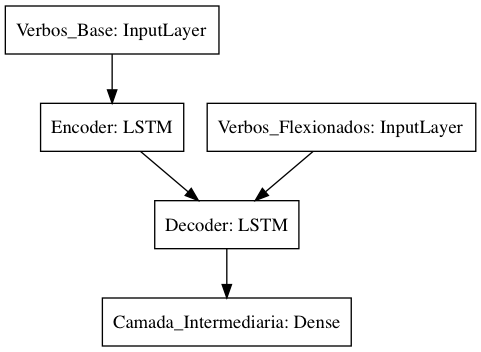
\includegraphics[width=0.6\textwidth]
{img/encoder-decoder.png}}
\caption{\label{fig:encoder-decoder} Arquitetura Final Utilizada.}
\end{figure}

\section{Metodologia para avaliação}
\label{sec:method}

 Para a avaliação dos resultados do modelo, foi utilizada uma técnica de validação cruzada chamada \textit{K-Fold} (\cite{kfold:2018}). A análise K-Fold permite que todos os verbos do corpus sejam testados. A técnica consiste, primeiramente, na formação de K subconjuntos de verbos mutuamente exclusivos de tamanhos próximos (idênticos caso a divisão por K seja exata). Em seguida, um desses subconjuntos é escolhido como o conjunto de teste enquanto que os K-1 restantes são utilizados como treino. O tamanho de K é definido a partir da escolha de proporção em que se deseja realizar a segmentação entre treino e teste, ou seja, para sempre manter a proporção de testes em 20\% de modo que estes verbos sejam sempre diferentes, o corpus precisa ser segmentado em 5 subconjuntos distintos. O desenho \ref{fig:kfold} exibe o particionamento dos \textit{datasets} segundo à proposta do algoritmo. 

\definecolor{blue}{RGB}{159, 192, 176}
\definecolor{green}{RGB}{160, 227, 127}
\definecolor{orange}{RGB}{243, 188, 125}
\definecolor{red}{RGB}{253, 123, 84}
\definecolor{nephritis}{RGB}{39, 174, 96}
\definecolor{emerald}{RGB}{46, 204, 113}
\definecolor{turquoise}{RGB}{39, 174, 96}
\definecolor{green-sea}{RGB}{22, 160, 133}
\definecolor{purple}{RGB}{181, 124, 215}
% Tikzstyles for Computation Graphs

% nodes
\tikzstyle{noop} = [circle, draw=none, fill=red, minimum size = 10pt]
\tikzstyle{op} = [circle, draw=red, line width=1.5pt, fill=red!70, text=black, text centered, font=\bf \normalsize, minimum size = 25pt]

\tikzstyle{opintense} = [circle, draw=red, line width=1.5pt, fill=red!150, text=black, text centered, font=\bf \normalsize, minimum size = 25pt]


%new style
\tikzstyle{gp} = [circle, draw=red, line width=4pt, text=black, text centered, font=\bf \normalsize, minimum size = 4.cm]

\tikzstyle{box} = [rectangle, draw=red, line width=1.5pt, fill=red!70, text=black, align=center, font=\bf \normalsize, minimum size = 45pt]

\tikzstyle{box2} = [rectangle, draw=black, line width=0.9pt, text=black, align=center, font=\bf \normalsize, minimum size = 20pt]

\tikzstyle{box3} = [rectangle, draw=black, line width=0.9pt, fill=black, text=black, align=center, font=\bf \normalsize, minimum size = 20pt]

\tikzstyle{state} = [circle, draw=blue, line width=1.5pt, fill=blue!70, text=black, text centered, font=\bf \normalsize, minimum size = 25pt]

\tikzstyle{output} = [circle, draw=purple, line width=1.5pt, fill=purple!70, text=black, text centered, font=\bf \normalsize, minimum size = 25pt]


\tikzstyle{gradient} = [circle, draw=nephritis, line width=1.5pt, fill=nephritis!60, text=black, text centered, font=\bf \normalsize, minimum size = 25pt]
\tikzstyle{textonly} = [draw=none, fill=none, text centered, font=\bf \normalsize]
\tikzstyle{boxtextonly} = [draw=none, fill=none, align=center, font=\bf \normalsize]

\tikzstyle{normal} = [circle, draw=black, line width=1.0pt, fill=none, text=black, text centered, font=\bf \normalsize, minimum size = 20pt]


% edges
\tikzstyle{tedge}  = [draw, thick, >=latex, ->]
\tikzstyle{tedge_dashed}  = [draw, thick, >=latex, ->, dashed]
\tikzstyle{nedge}  = [draw, thick, >=latex]
\tikzstyle{nedge_dashed}  = [draw, thick, >=latex, dashed]


% namedscope
\tikzstyle{namedscope} = [circle, draw=orange, line width=1.5pt, fill=orange!60, align=center, inner sep=0pt]
\begin{figure}[ht!]
\centering

\scalebox{1.0}{
\begin{tikzpicture}[H]

%first
\node[box3] (box1) {};
\node[box2, right=0pt of box1] (box2) {};
\node[box2, right=0pt of box2] (box3) {};
\node[box2, right=0pt of box3] (box4) {};
\node[box2, right=0pt of box4] (box5);

%second
\node[box2, below=15pt of box1] (box6) {};
\node[box3, right=0pt of box6] (box7) {};
\node[box2, right=0pt of box7] (box8) {};
\node[box2, right=0pt of box8] (box9) {};
\node[box2, right=0pt of box9] (box10);

%third
\node[box2, below=15pt of box6] (box11) {};
\node[box2, right=0pt of box11] (box12) {};
\node[box3, right=0pt of box12] (box13) {};
\node[box2, right=0pt of box13] (box14) {};
\node[box2, right=0pt of box14] (box15);

%fourth
\node[box2, below=15pt of box11] (box16) {};
\node[box2, right=0pt of box16] (box17) {};
\node[box2, right=0pt of box17] (box18) {};
\node[box3, right=0pt of box18] (box19) {};
\node[box2, right=0pt of box19] (box20);

%fifth
\node[box2, below=15pt of box16] (box21) {};
\node[box2, right=0pt of box21] (box22) {};
\node[box2, right=0pt of box22] (box23) {};
\node[box2, right=0pt of box23] (box24) {};
\node[box3, right=0pt of box24] (box25);

%legenda
\node[box2, right=35pt of box10] (box26) {};
\node[textonly, right=5pt of box26] (box27) {Treino};
\node[box3, below=10pt of box26] (box28) {};
\node[textonly, right=5pt of box28] (box29) {Teste};



\end{tikzpicture}
}\caption{Técnica de segmentação do Corpus via K-Fold} 
\label{fig:kfold}
\end{figure}

Além disso, há ainda a vantagem do algoritmo de estratificação, ou seja, a certeza de que, em cada um dos treinamentos, as proporções das classes de verbos se mantenham no treinamento. Isso significa que, por exemplo, a classe de irregularidades do verbo “\textit{testar}” (testar $\rightarrow$ testo) que possui 20 verbos, terá sempre 16 verbos verbos no treinamento e 4 no teste. Assim, após os 5 treinamentos diferentes, todos os verbos da classe foram testados e fica garantido que havia verbos dessa classe no treinamento.

\subsection{Métrica de avaliação}

Para a avaliação dos resultados, considerou-se a métrica de \textit{Acurácia}. A acurácia pode ser obtida através da fórmula:

\begin{equation}
    Acurácia = \frac{contagem(acertos)}{contagem(total)}
\end{equation}

Ainda, define-se como um acerto um verbo predito exatamente igual ao esperado.

\section{Resultados}
\label{sec:resultado}
Como há um fator de aleatoriedade nas inicializações dos pesos, e também como os verbos de treino e teste são sorteados pelo algoritmo no momento da segmentação do K-Fold, os resultados da rede podem variar. Para a verificação dos resultados levando em consideração as variações, foram realizadas 30 análises K-Fold. Isso significa que cada verbo foi testado 30 vezes. Em média, temos que o modelo acerta 13.55\% dos verbos. Entretanto, a Fig. \ref{fig:acc} mostra um gráfico do tipo \textit{boxplot} (\cite{2004:bussab}) onde podemos verificar a variação da acurácia. Na figura, podemos notar que a taxa média de acerto do modelo desenvolvido se concentra entre 12.5-14.7\%, mas chega até 17\%.

\begin{figure}[H]
  \centering
  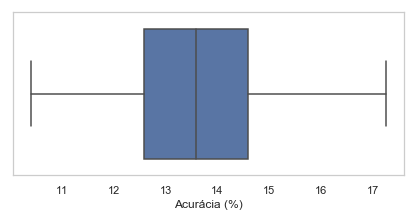
\includegraphics[width=0.6\linewidth]{img/mean_accuracy.png}
  \caption{Acurácia Para Todos os Verbos}
  \label{fig:acc}
\end{figure}

Ainda, agrupando todas as classes irregulares em apenas uma, é possível avaliar o desempenho do modelo comparativamente entre o grupo dos verbos regulares e o grupo de irregulares.
Nesse caso, a Fig. \ref{fig:boxplotsclasses} e a Tab. \ref{tab:acuraciamedia} mostram que o modelo obteve resultados melhores para a classe dos verbos regulares. 

\begin{figure}[H]
\begin{floatrow}
\ffigbox{%
  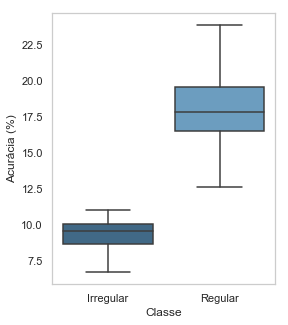
\includegraphics[width=0.8\linewidth]{img/boxplot_irregular_vs_regular.png}%
}{%
  \caption{Boxplots Para Acurácias por Classe}%
  \label{fig:boxplotsclasses}
}
\capbtabbox{%
\begin{tabular}{lll}
 & \textbf{Regulares} & \textbf{Irregulares} \\ \hline
\textbf{Acurácia Média} & 17.88 \% & 9.23 \% \\
\textbf{Acurácia DP} & 2.30 \% & 1.15 \% \\
\textbf{Acurácia Min}& 12.65 \% & 6.70 \%\\
\textbf{Acurácia Max}& 23.83 \% &  11.00 \%\\ \hline\\
& & \\ 
& & \\
& & \\
& & \\
\end{tabular}
}{%
  \caption{Acurácias Médias por Classe com Desvio Padrão (DP)}%
  \label{tab:acuraciamedia}
}
\end{floatrow}
\end{figure}




\subsection{Acurácia em cada classe}
\label{sec:prop}

Também é interessante avaliar o desempenho do modelo em cada uma das 16 classes formadas. Na Fig. \ref{fig:kfoldprop} observamos as acurácias de cada classe ordenadas pela proporção das mesmas no corpus. Nota-se que, apesar de a classe regular apresentar a maior proporção no corpus, as classes com maior acurácia são as classes dos verbos “botar” e “seguir”. Para avaliar a correlação entre a proporção no corpus e a acurácia foi utilizado o coeficiente de correlação de Pearson (\cite{2004:bussab}). Esse coeficiente assume valores entre -1 e 1, sendo que valores próximos às extremidades indicam maior correlação e valores próximos a zero indicam que as variáveis independem linearmente uma da outra. Para a interpretação do valor obtido utilizaremos a seguinte escala (\cite{pearson:1989}):

\begin{itemize}
    \item 0.9 positivo ou negativo indica uma correlação muito forte.
    \item0.7 a 0.9 positivo ou negativo indica uma correlação forte.
    \item0.5 a 0.7 positivo ou negativo indica uma correlação moderada.
    \item0.3 a 0.5 positivo ou negativo indica uma correlação fraca.
    \item0 a 0.3 positivo ou negativo indica uma correlação desprezível.
\end{itemize}

O coeficiente de correlação observado entre essas variáveis foi de \textbf{0.42}, o que indica uma correlação \textit{fraca}. 

\begin{figure}[H]
  \centering
  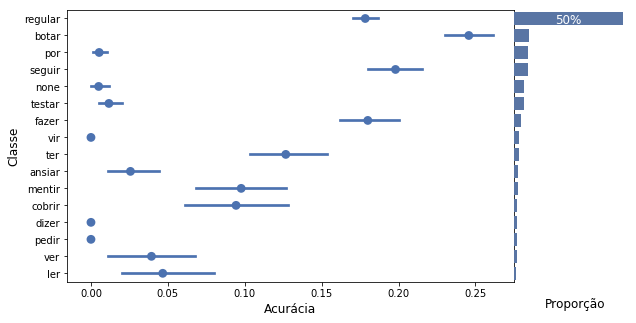
\includegraphics[width=0.8\linewidth]{img/proporxacc.png}
  \caption{Acurácia Para Cada Classe}
  \label{fig:kfoldprop}
\end{figure}

Para a análise dos resultados obtidos, utilizaremos o experimento K-Fold de acurácia total mais alta como referência (17\%, vide apêndice \ref{ap:results}). Como se pode observar, diferentes tipos de erros podem acontecer, sendo que alguns são piores do que outros. Vejamos, por exemplo, o verbo “parecer” (com transcrição fonética e RAD + VT = “parese”). Nesse caso vemos que o modelo produziu a forma “peresu”. Nota-se que essa transformação em que o modelo errou alguns traços de um único fone, é diferente do erro que ocorre com o verbo “retrair” (com transcrição fonética e RAD + VT = “hetrai”), para o qual o modelo produziu a forma “setEruu”. Vemos que no segundo caso, a forma produzida é praticamente incompreensível. %Desse modo, ao avaliarmos as diferentes classes de verbos, falaremos em \textit{erros incompreensíveis} para descrever os verbos cujas formas preditas apresentam erros de difícil interpretabilidade. 

Ao analisar os erros ocorridos na classe do verbo “Pôr” (Tab. \ref{tab:class_por}), verifica-se que 7/26 dos erros cometidos foram erros de \textit{regularização}, ou seja, o modelo se confundiu com a classe mais presente (a classe dos verbos regulares) e manteve o padrão de flexão regular.

\begin{table}[H]
\begin{tabular}{lll}
\multicolumn{1}{c}{Input} & \multicolumn{1}{c}{Output} & \multicolumn{1}{c}{Alvo} \\ \hline
kompo                     & kompu                      & kompoNu                  \\
despo                     & despu                      & despoNu                  \\
espo                      & espu                       & espoNu                   \\
antepo                    & antepu                     & antepoNu                 \\
supo                      & supu                       & supoNu                   \\
prosupo                   & prosupu                    & prosupoNu                \\
propo                     & propu                      & propoNu                  \\ \hline
\end{tabular}
\caption{Erros de regularização na classe do verbo “Pôr”}
\label{tab:class_por}
\end{table}

Em seguida, analisamos os verbos sem agrupamento (na Fig. \ref{fig:kfoldprop}, “none”). A acurácia baixa nesta classe era esperada pois não havia outros verbos no corpus para que o modelo conseguisse detectar possíveis padrões para fazer predições corretas. A Tab. \ref{tab:none} exibe alguns exemplos de erros nesta classe.

\begin{table}[H]
\begin{tabular}{lll}
\multicolumn{1}{c}{Input} & \multicolumn{1}{c}{Output} & \multicolumn{1}{c}{Alvo} \\ \hline
kabe                      & kabu                       & kaibu                    \\
idea                      & adeiu                      & ideiu                    \\
esta                      & estu                       & estou                    \\
traze                     & trasu                      & tragu                    \\
prove                     & provu                      & proveNu                  \\
estrea                    & estreiu                    & estrEiu                  \\ \hline
\end{tabular}
\caption{Exemplos de erros na classe sem agrupamento}
\label{tab:none}
\end{table}

Exemplos de erros na classe do verbo “testar” podem ser vistos na Tab. \ref{tab:class_testar}. Chama a atenção que, para o verbo “pegar”, o modelo acertou a flexão irregular transformando a vogal anterior meio-fechada em meio-aberta (e $\rightarrow$ \textepsilon), porém não acertou o traço de vozeamento para caracterizar o fone “g” ao invés de “k”, o que resultou na flexão equivocada de pegar $\rightarrow$ pEku.

\begin{table}[H]
\begin{tabular}{lll}
\multicolumn{1}{c}{Input} & \multicolumn{1}{c}{Output} & \multicolumn{1}{c}{Alvo} \\ \hline
seka                      & seku                       & sEku                     \\
leva                      & levu                       & lEvu                     \\
sega                      & segu                       & sEgu                     \\
fexa                      & fexu                       & fExu                     \\
pega                      & pEku                       & pEgu                     \\ \hline
\end{tabular}
\caption{Exemplos de erros na classe do verbo “testar”}
\label{tab:class_testar}
\end{table}

A classe do verbo “vir”, por sua vez, apresentou 5/11 de erros por regularização. Além disso, é interessante que para o verbo “revir” (\textit{hevi}) tenha flexionado como \textit{“heviju”}, flexão próxima ao grupo do verbo “ver”. A Tab. \ref{tab:class_vir} exibe alguns exemplos de erros nesta classe.

\begin{table}[H]
\begin{tabular}{lll}
\multicolumn{1}{c}{Input} & \multicolumn{1}{c}{Output} & \multicolumn{1}{c}{Alvo} \\ \hline
sobrevi                   & sobrevu                    & sobreveNu                \\
hevi                      & heviju                     & heveNu                   \\
adivi                     & adivu                      & adiveNu                  \\
avi                       & aviu                       & aveNu                    \\
provi                     & provu                      & proveNu                  \\ \hline
\end{tabular}
\caption{Exemplos de erros da classe “vir”}
\label{tab:class_vir}
\end{table}


\subsection{Acurácia e comprimento médio dos verbos nas classes}

Como o coeficiente de \textit{Pearson} observado entre a proporção das classes no corpus e a acurácia indicou uma correlação fraca, podemos buscar por outras variáveis que também possam influenciar no desempenho do modelo. Uma delas é o comprimento dos verbos. O verbo “3ntret3Nu” (entretenho), por exemplo, contém 9 fones para serem preditos. Como cada fone contém 20 traços, no total o modelo tem que conseguir prever 180 números. O verbo “falu” (falo), em contrapartida, possui 4 fones, ou seja, 80 números a serem preditos. Dessa forma, é natural pensar que quanto maior o número de predições necessárias, maior a probabilidade do modelo cometer algum erro. Com isso, a Figura \ref{fig:kfoldprop} exibe as acurácias das classes ordenadas de acordo com os comprimentos médios das mesmas. Na figura vemos que os grupos apresentam comprimentos médios que variam de 5 a 8 fones, mas com barras de confiança com limites próximos, indicando uma certa homogeneidade nesse aspecto.

No caso desse estudo, o coeficiente de \textit{Pearson} obtido foi de \textbf{0.39}, o que indica uma correlação também fraca entre estas variáveis. Entretanto, vemos nas barras de confiança que há pouca diferença significativa entre os comprimentos médios das classes. Além disso, é interessante notar que a classe em que o modelo apresentou melhor desempenho (a classe de “botar”) é simultaneamente uma classe com alta proporção no corpus e também apresenta o comprimento médio mais baixo do grupo.

\begin{figure}[H]
  \centering
  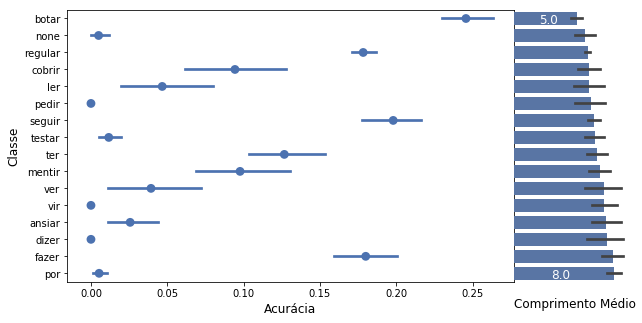
\includegraphics[width=0.8\linewidth]{img/comp_acc.png}
  \caption{Acurácia por Comprimento Médio}
  \label{fig:kfoldprop}
\end{figure}


% colocar no apendice os resultados
\section{Outros erros relevantes}
\label{sec:interesting}

Alguns erros interessantes como troca de classes e regularizações já foram apresentados na Seção \ref{sec:prop}, mas ainda há outros erros que merecem destaque. (Ver Apêndice \ref{ap:results} para tabela completa com Classe, Input, Output e Alvo)

Na classe de verbos sem agrupamento, um erro notável foi a flexão realizada para o verbo trazer (“trasu”), o que mostra que o modelo identificou o padrão de flexão da classe do verbo “fazer”. 

Na classe do verbo “pedir”, o modelo apresentou a flexão “espidu” para o verbo “expedir” (com alvo “espEsu” - “expeço”), o que denota uma possível confusão com a classe do verbo “conseguir”.

Nos verbos regulares nota-se a presença de vários erros devido à troca de apenas um traço fonético. Como por exemplo para o verbo “convidar”, o \textit{output} resultante foi “konviru” (trocou [\textbf{d}] - oclusiva, alveolar, sonora; por [\textbf{r}] - tepe, alveolar, sonora) . Para o verbo “convencer”, “konfensu” (trocou [\textbf{v}] - fricativa, lab. dental, sonora; por [\textbf{f}] - fricativa, lab. dental, surda).

Para os verbos da classe do verbo “seguir“, três verbos foram flexionados de acordo com a família do verbo “testar”. São eles: “ferir” (fEru), “vestir” (vEstu) e “repetir” (hepEtu).

A classe do verbo “ver” também apresentou erros interessantes: a confusão com a classe do verbo “vir” nos verbos “prever” (“preveNu”) e “entrever” (“entreveNu”). Também não acertou o alvo do verbo “rever” (hefexu), ficou faltando o traço de sonoridade nas duas últimas consoantes.

\section{Discussão}
\label{sec:discuss}

Durante a execução do presente trabalho, foi divulgado um estudo semelhante realizado pelos pesquisadores \cite{kirov:2018}. Nesse estudo, Kirov e Cotterell revisitam a questão dos verbos irregulares do inglês utilizando a arquitetura \textit{Encoder-Decoder}. Em razão da similaridade entre os estudos, é interessante pautar a discussão dos resultados obtidos através de uma comparação entre os mesmos. 

 No grupo dos verbos regulares, \cite{kirov:2018} obtiveram um desempenho próximo a 100\%. Entretanto, ao observarmos exclusivamente o desempenho no grupo dos verbos irregulares, a acurácia cai para 28.6\%. \cite{kirov:2018} explicam que os erros obtidos nessa circunstância foram erros de \textit{regularização}, e que em nenhum momento o modelo misturou regulares e irregulares como em “\textit{gaved}” (erro observado e criticado no modelo de \cite{rumelhart:1986}). Em números absolutos, os autores apresentaram um corpus composto por 4039 verbos (aproximadamente 10 vezes maior que o utilizado nesta pesquisa), sendo 168 destes considerados irregulares. Além disso, \cite{kirov:2018} realizaram uma partição aleatória tripla no corpus com proporções 80-10-10 para treino, desenvolvimento e teste. Desse modo, a base de teste dos pesquisadores continha apenas em torno de 17 verbos irregulares. Com uma acurácia de 28\%, isso significa que o modelo \textit{Encoder-Decoder} apresentado pelos autores acertou apenas cinco verbos irregulares. Sobre estes verbos, três deles eram verbos derivados de outros através de prefixação: \textit{retell} (derivado de \textit{tell}), \textit{partake} (derivado de \textit{take}) e \textit{withdraw} (derivado de \textit{draw}). Outro era o verbo \textit{sling}, similar a outros verbos presentes no treino (\textit{fling}, por exemplo). O último foi o verbo \textit{forsake}, cuja terminação se assemelha bastante ao verbo \textit{take}.

Além do modelo \textit{Encoder-Decoder} apresentado, \cite{kirov:2018} também reproduziram o modelo de regras de \cite{Albright2003RulesVA} (comentado na Seç. \ref{sec:compmot}) como referência (\textit{benchmark}) utilizando o mesmo corpus. Segundo os autores, para este modelo a acurácia dentre os verbos regulares ficou em torno de 95\%, porém não foi capaz de acertar nenhum verbo irregular em nenhuma das três partições realizadas. 

Em termos de pré-processamento, \cite{kirov:2018}
não explicitam a codificação utilizada, mas explicam que não utilizaram traços fonéticos como dados de entrada para a rede. A base de dados utilizada pelos autores foi a \textit{CELEX}, retirada de \cite{Baayen1993TheCL}, e era composta pelos verbos transcritos com a notação do AFI. 

Voltando ao modelo desenvolvido nesta pesquisa, observamos que a acurácia obtida no grupo dos verbos regulares foi a mais baixa em comparação aos demais trabalhos aqui referidos (com uma acurácia média igual a 13.55\% e máxima = 17\%). Entretanto, isto pode ser explicado em razão do tamanho do corpus necessário para o aprendizado em arquiteturas mais complexas, como é o caso do \textit{Encoder-Decoder}. Como visto, o modelo de \cite{kirov:2018} utilizou 4039 verbos para a tarefa (um corpus 10 vezes maior que o utilizado nesta pesquisa). Entretanto, como a ordem de grandeza obtida (423 verbos) estava próxima à ordem do conjunto de \cite{rumelhart:1986} (506 verbos), acreditava-se que o corpus obtido seria suficiente para a obtenção de acurácias mais altas. 

Com relação aos verbos irregulares, apesar da acurácia média obtida ter sido 9.23\%, em números absolutos isso representa em torno de 20 verbos. Dessa forma, é difícil comparar os dois modelos nessa questão. Se, por um lado, o montante de verbos regulares obtidos por \cite{kirov:2018} os levou a quase 100\% de acurácia nesse grupo, também foi um fator desfavorável para o desempenhoo no grupo dos verbos irregulares. Também pode-se questionar se os cinco verbos corretos obtidos por \cite{kirov:2018} refletem de fato o potencial de 23\% de acurácia do modelo. Certamente a discussão seria mais interessante caso tivéssemos uma acurácia média com desvio-padrões, como foi apresentado neste trabalho. Em comparação com os resultados do \textit{benchmark} de \cite{kirov:2018} (baseado no modelo de \cite{Albright2003RulesVA}), o modelo apresentado nesta pesquisa apresentou desempenho melhor nesse quesito (9.23\% contra 0\%). 

No que diz respeito aos tipos de erros encontrados, pode-se dizer que alguns erros observados nesta pesquisa mostram-se bastante incompreensíveis de um ponto de vista linguístico em comparação aos apresentados por \cite{kirov:2018} (erros como “\textit{aAsaxu}”, como \textit{output} para o verbo “\textit{analisar}”). Entretanto, como os processos de codificação e decodificação, bem como os tamanhos dos \textit{corpus} e os objetos dos estudos são diferentes (traços fonéticos x fonemas), também seria injusta uma comparação entre os modelos nesse sentido.

Sobre o fato das métricas das correlações obtidas entre acurácia e tamanho médio e proporção no corpus não terem se mostrado fortes,
 chama a atenção a classe do verbo “botar”. Essa classe, além ter apresentado a maior acurácia, apresenta também proporção no corpus  alta e é também a classe com comprimento médio mais baixo. Desse modo, supõe-se que estes fatores combinados tenham levado a esse resultado. Uma análise multivariada poderia ser feita para investigar a suposição em mais profundidade.

Para concluir a discussão, pode-se dizer que o desempenho do modelo \textit{Encoder-Decoder} está bastante condicionado à quantidade do corpus disponível. De certo que para qualquer modelo de Rede Neural, quanto maior o número de exemplos, melhor. Entretanto, vemos também que quanto mais profunda a arquitetura do modelo de Rede Neural, maior a demanda por mais exemplos. Ainda, vimos que a questão da proporção da classe de verbos irregulares mostrou-se relevante. Desse modo, os resultados obtidos nesta pesquisa não permitem dizer que o modelo \textit{Encoder-Decoder} seja adequado para esta tarefa. Contudo, pode-se argumentar que, como os processos de codificação e decodificação são módulos independentes da arquitetura, essa conclusão a respeito do modelo \textit{Encoder-Decoder} seria injusta. Além disso, para que pudéssemos chegar a conclusões mais contundentes, mais experimentos deveriam ser realizados. Dito isto, direções para possíveis trabalhos futuros serão abordadas no próximo capítulo (Cap. \ref{ch:08}). 

  
\chapter{Conclusão}
\label{ch:08}

Este trabalho teve como principal objetivo estudar a questão do aprendizado de verbo irregulares do Português Brasileiro através da arquitetura \textit{Encoder-Decoder} (\cite{enc-dec:2014}, \cite{seq2seq:2014}). 

Para tanto, o escopo desta pesquisa foi restringido à 1$^{a}$ pessoa do singular, no tempo presente e modo indicativo. Em seguida, um corpus com 423 verbos foi criado e transcrito para uma representação fonética utilizando a metodologia desenvolvida no Capítulo \ref{ch:02}. O corpus criado foi primeiramente particionado segundo classes de irregularidade. No total, quinze classes irregulares foram formadas. A proporção de verbos regulares e irregulares no corpus montado foi de respectivamente 50.6\% e 49.4\%. Após a coleta e organizacão dos verbos, os mesmos foram pré-processados para serem introduzidos na camada de \textit{input} do modelo. 

O modelo \textit{Encoder-Decoder} foi configurado da seguinte maneira: As redes \textit{Encoder} e \textit{Decoder} são ambas do tipo LSTM's de dimensão latente de 256 nós. Para o treinamento foram utilizadas 300 épocas com lotes de 128 verbos por vez. O modelo foi otimizado com o algoritmo \textit{Adam} disponível na API do \textit{Keras} (\cite{chollet2015keras}) com hiperparâmetros pré-definidos na documentação. A função de custo utilizada foi a Entropia Cruzada Binária.

Para a avaliação do modelo construído, foi utilizada a técnica de validação cruzada chamada \textit{K-fold} (\cite{kfold:2018}), que permite que todos os verbos do corpus sejam testados pelo modelo. A métrica de avaliação escolhida foi a acurácia. Para considerar as variações possíveis durante os treinamentos, o algoritmo K-fold foi executado trinta vezes. Desse modo, foi possível estudar o comportamento médio do modelo nas diferentes classes do estudo.

A acurácia máxima atingida pelo modelo foi de 17\% considerando todos os verbos do corpus ($73/423$). Considerando apenas verbos regulares x verbos irregulares, o desempenho do modelo foi melhor no primeiro grupo, sendo as respectivas acurácias médias 17.88\% e 9.23\%. Considerando-se todas as classes do estudo, destaca-se a classe do verbo “botar” que, além de possuir alta proporção de exemplos no Corpus, é também a classe com menor comprimento médio. Ainda, foram observados alguns erros interessantes de troca de famílias nos verbos irregulares, como por exemplo: repetir (hepeti $\rightarrow$ hepEtu). Também ocorreram alguns erros de super-regularização (x). 

Durante a sessão de discussão (\ref{ch:05}), observamos que o tamanho do corpus obtido mostrou-se incompatível com a arquitetura \textit{Encoder-Decoder}. Entretanto, questiona-se se é razoável que um modelo computacional desenvolvido para esta tarefa necessite de um número muito maior de exemplos para o aprendizado. Por outro lado, observa-se que os módulos de pré e pós processamento dos verbos são independentes da arquitetura proposta. Neste sentido, pode-se argumentar que o resultado obtido nesta pesquisa não é conclusivo quanto ao desempenho do \textit{Encoder-Decoder}. 

Para pesquisas futuras, ficam algumas sugestões:

\begin{enumerate}

\item Obtenção de um corpus maior para a língua portuguesa
para que o algoritmo apresentado nesta pesquisa possa ser reavaliado;

\item Desenvolvimento de novos algoritmos de pré e pós processamento dos verbos. Outras representações vetoriais podem ser desenvolvidas. Uma opção é adicionar uma camada de \textit{embedding} (ref) antes da camada de \textit{input} do \textit{Encoder}; 

\item Realização de um teste psicolinguístico com verbos irregulares inventados para uma comparação entre as predições do modelo e as opiniões de falantes da língua;

\item Construção de um modelo do tipo \textit{Transformer} (\cite{Vaswani2017AttentionIA}). A arquitetura \textit{Transformer} é considerada a nova arquitetura estado-da-arte para modelos de tradução automática. 

\end{enumerate}

Para concluir, esperamos que a presente pesquisa tenha apresentado importantes contribuições para o tema do aprendizado de verbos irregulares dentro do domínio dos modelos de Redes Neurais Artificiais. No campo da Linguística, a construção de um corpus adequado e a execução desta tarefa para o Português Brasileiro foram certamente eventos inéditos nesta língua. 
% Bibliografia
\setcitestyle{square}
 \singlespacing   % espaçamento simples
\bibliographystyle{marcos4} % citação bibliográfica textual
\bibliography{references}  % associado ao arquivo: 'bibliografia.bib'
\clearpage

%\pagenumbering{gobble}
\appendix

\chapter{Tabela de Transcrição Fonética de Rumelhart e McClelland}
\label{apendice:rumelhart}
\begin{figure}
    \centering
    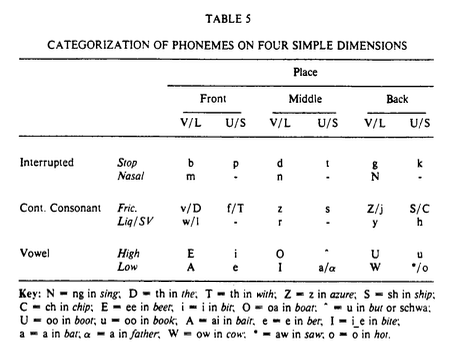
\includegraphics[scale=0.8]{img/rumelhartpreprocess.png}
    \caption{Tabela de Pré-Processamento retirada de \cite{rumelhart:1986} (pág. 235)}
    \label{fig:preprocess-rumelhart}
\end{figure}

\chapter{Corpus}
\label{ap:corpus}
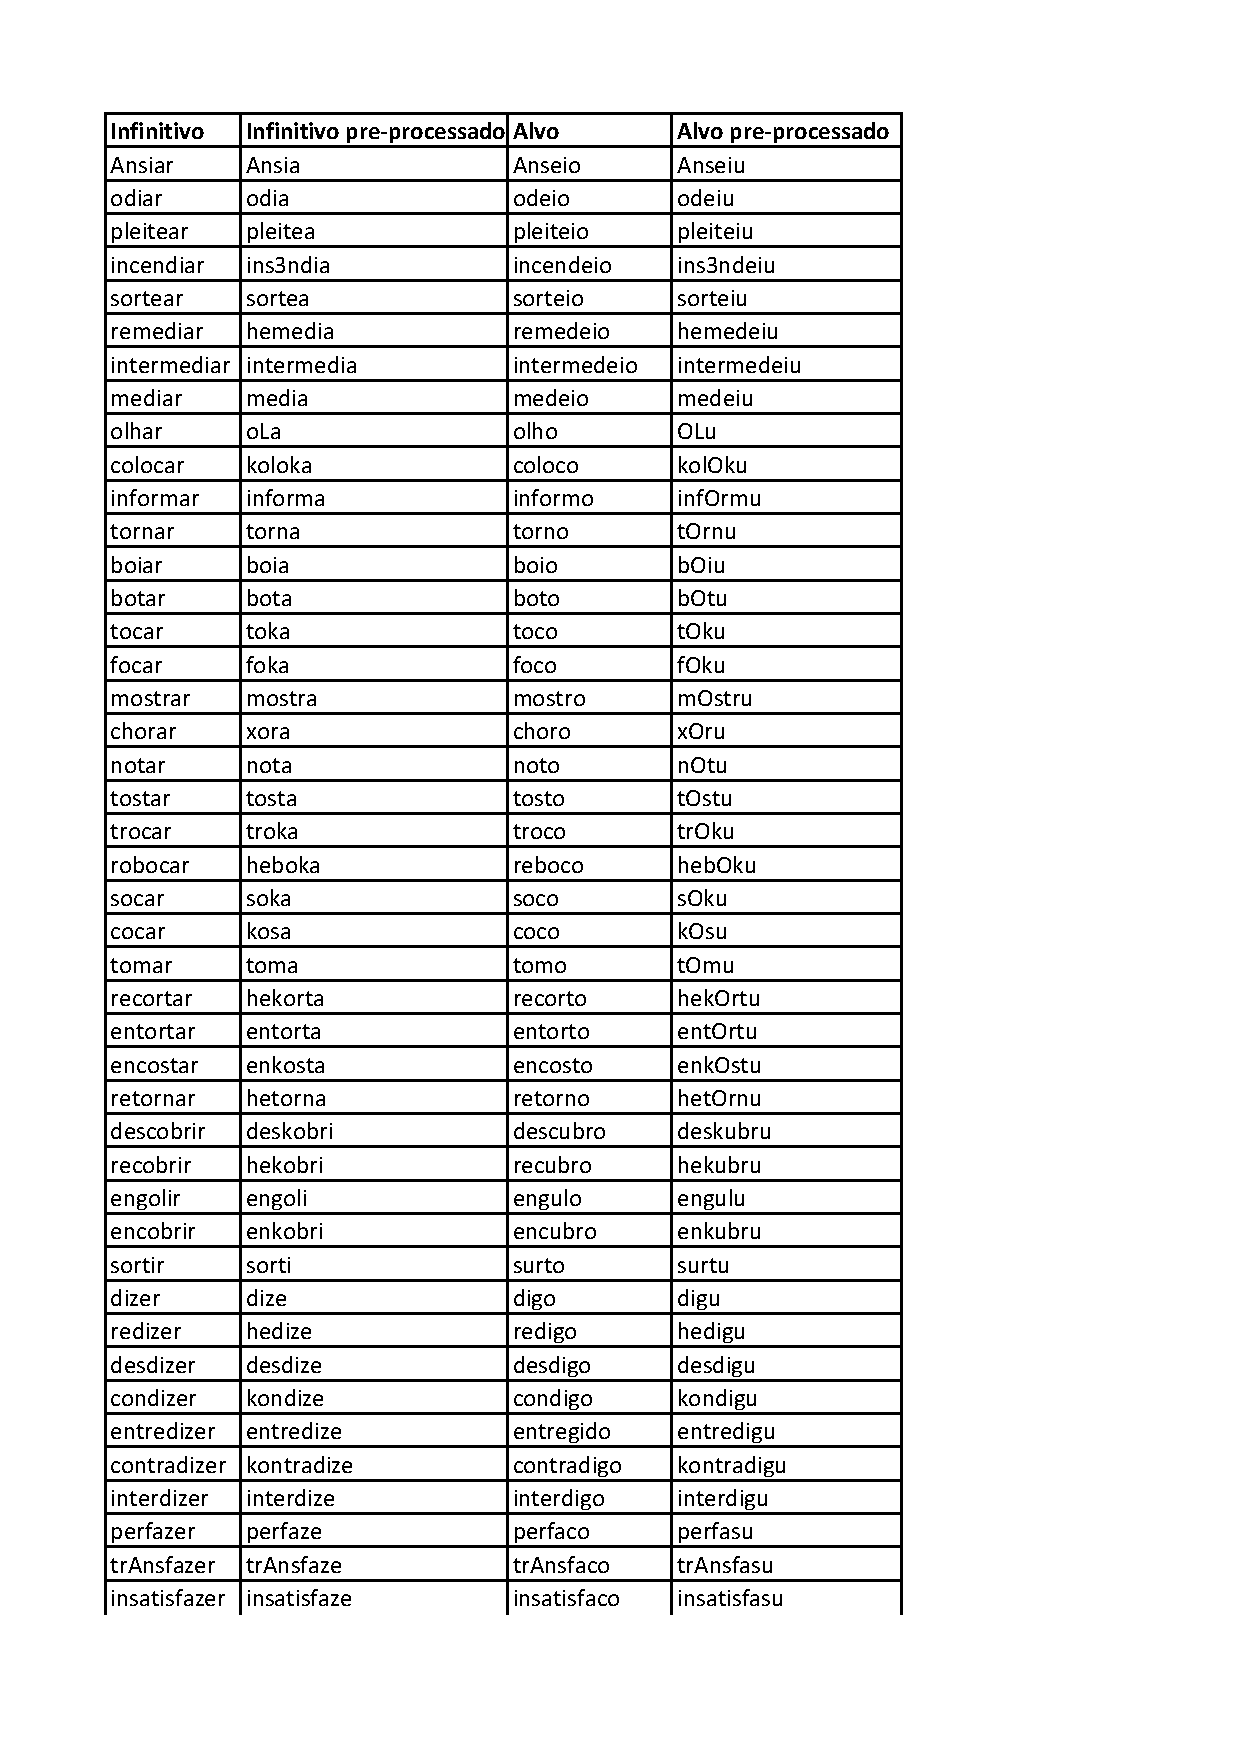
\includepdf[pagecommand={\thispagestyle{plain}},
  pages=-]{corpus_dissertacao.pdf}

\chapter{Resultados das Decodificações}
\label{ap:results}
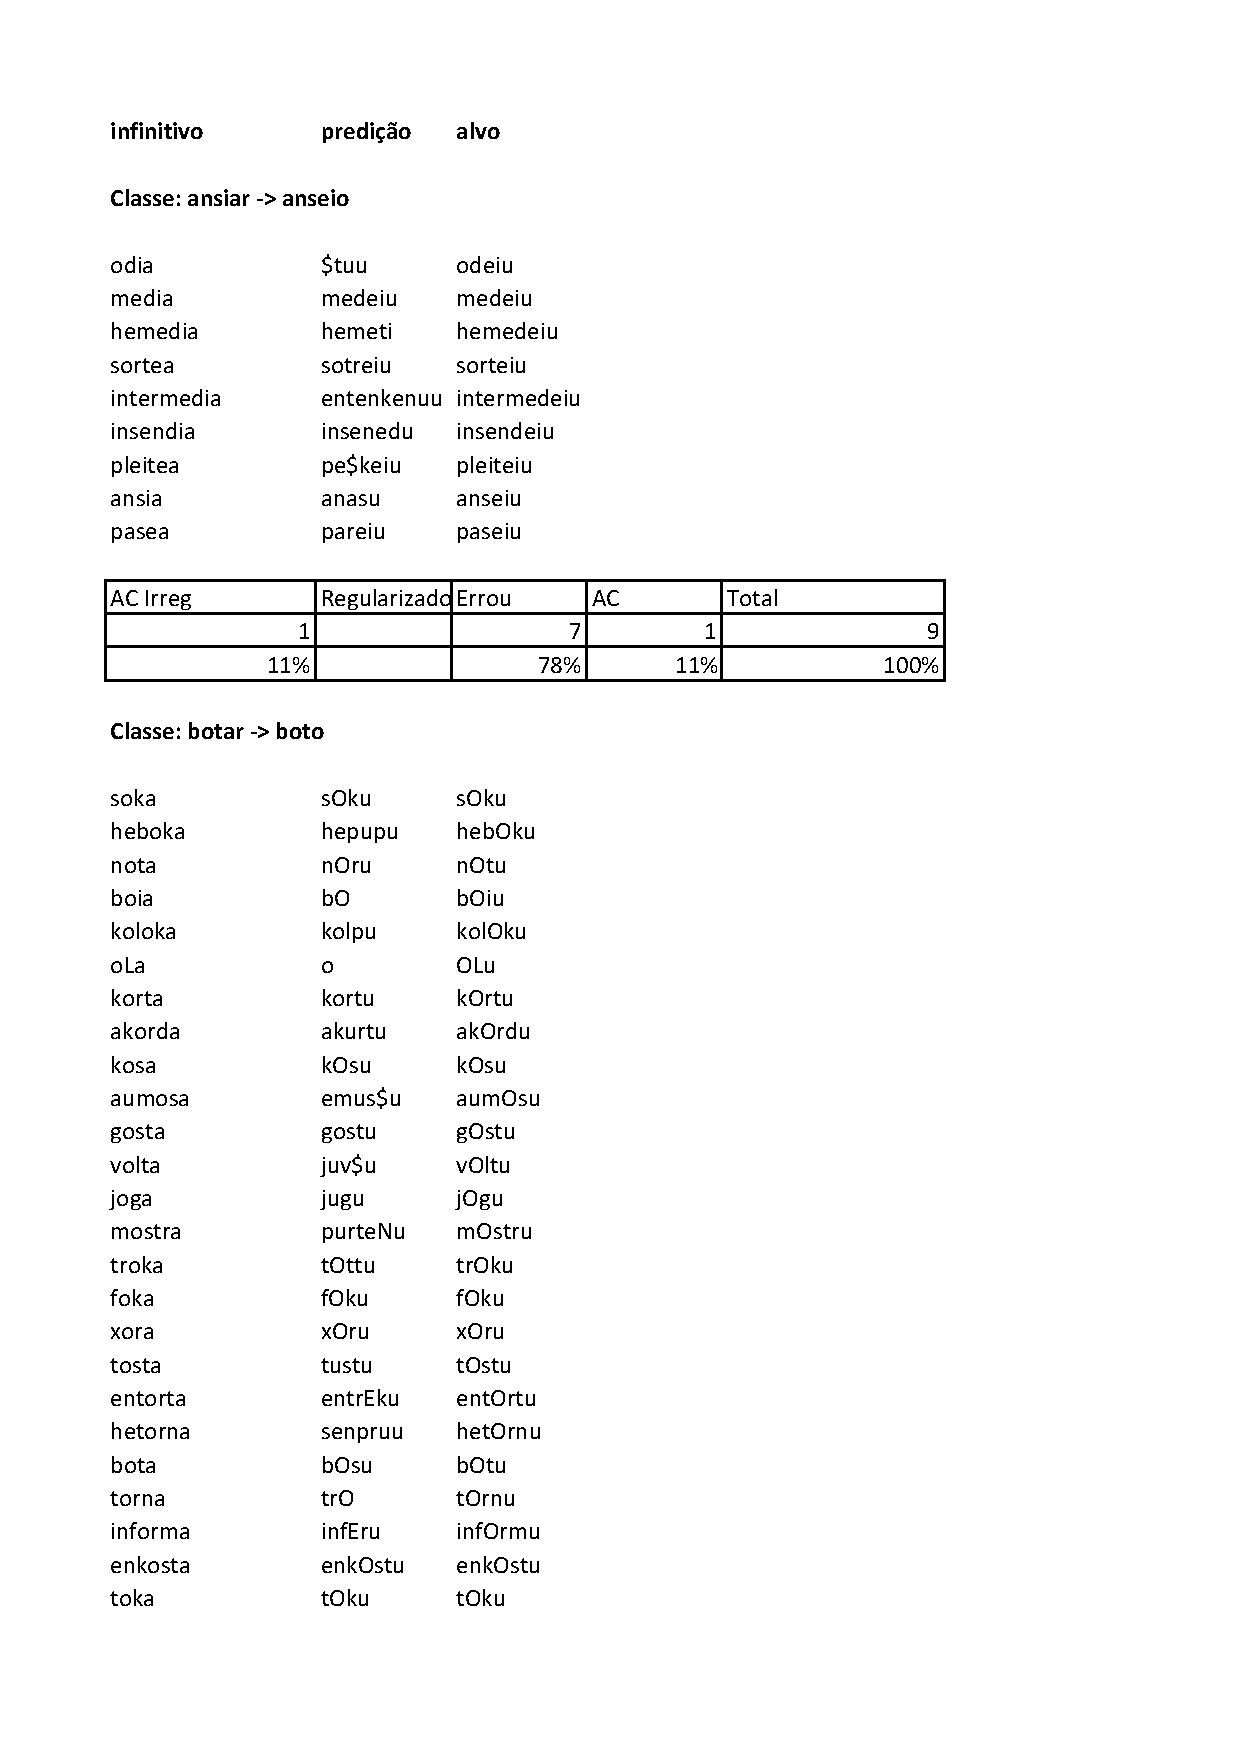
\includepdf[pagecommand={\thispagestyle{plain}},
  pages=-]{results_analysis_by_family.pdf}

\backmatter
% cabeçalho para os apendices

% ---------------------------------------------------------------------------- %


% ---------------------------------------------------------------------------- %


% \printindex   % imprime o índice remissivo no documento 

\end{document}
